\documentclass[10pt]{article}
\usepackage[utf8]{inputenc}
\usepackage[T1]{fontenc}
\usepackage{amsmath}
\usepackage{amsfonts}
\usepackage{amssymb}
\usepackage[version=4]{mhchem}
\usepackage{stmaryrd}
\usepackage{graphicx}
\usepackage[export]{adjustbox}
\graphicspath{ {./images/} }
\usepackage{hyperref}
\hypersetup{colorlinks=true, linkcolor=blue, filecolor=magenta, urlcolor=cyan,}
\urlstyle{same}

\title{Answers to Water Distribution Operator Questions }

\author{}
\date{}


\DeclareUnicodeCharacter{0131}{$\imath$}

\begin{document}
\maketitle
\section{System Information/Components}
\section{Sample Questions for Level I-Answers}
\begin{enumerate}
  \item Answer: c. feet.
\end{enumerate}

Reference: Basic Science Concepts and Applications, 4th edition. 2010. Nicholas G. Pizzi, Editor. American Water Works Association. Hydraulics 3.

\begin{enumerate}
  \setcounter{enumi}{1}
  \item Answer: a. a map.
\end{enumerate}

Reference: Water Transmission and Distribution, 4th edition. 2010. Larry Mays, Editor. American Water Works Association. Glossary.

\begin{enumerate}
  \setcounter{enumi}{2}
  \item Answer: d. Air-and-vacuum relief valve
\end{enumerate}

Reference: Water Transmission and Distribution, 4th edition. 2010. Larry Mays, Editor. American Water Works Association. Chapter 6.

\begin{enumerate}
  \setcounter{enumi}{3}
  \item Answer: a. cathodic protection.
\end{enumerate}

Reference: Water Transmission and Distribution, 4th edition. 2010. Larry Mays, Editor. American Water Works Association. Chapter 2.

\begin{enumerate}
  \setcounter{enumi}{4}
  \item Answer: a. Early morning
\end{enumerate}

Reference: Water Transmission and Distribution, 4th edition. 2010. Larry Mays, Editor. American Water Works Association. Chapter 5.

\section{Sample Questions for Level II-Answers}
\begin{enumerate}
  \item Answer: a. pressure head.
\end{enumerate}

Reference: Pumping: Fundamentals for the Water \& Wastewater Maintenance Operator Series. 2001. Frank R. Spellman and Joanne Drinan. Technomic Publishing Company.

\begin{enumerate}
  \setcounter{enumi}{1}
  \item Answer: b. pump head.
\end{enumerate}

Reference: Pumping: Fundamentals for the Water \& Wastewater Maintenance Operator Series. 2001. Frank R. Spellman and Joanne Drinan. Technomic Publishing Company.

\begin{enumerate}
  \setcounter{enumi}{2}
  \item Answer: d. roughness that retards flow due to friction.
\end{enumerate}

Reference: Water Transmission and Distribution, 4th edition. 2010. Larry Mays, Editor. American Water Works Association. Chapter 2.

\begin{enumerate}
  \setcounter{enumi}{3}
  \item Answer: b. Push-on joint
\end{enumerate}

Reference: Water Transmission and Distribution, 4th edition. 2010. Larry Mays, Editor. American Water Works Association. Chapter 2. 5. Answer: d. air gap, RPZ, DCVA, and VB.

Reference: Water Transmission and Distribution, 4th edition. 2010. Larry May Editor. American Water Works Association. Chapter 11.

\section{Sample Questions for Level III-Answers}
\begin{enumerate}
  \item Answer: c. proportionately.
\end{enumerate}

Reference: Pumping: Fundamentals for the Water \& Wastewater Maintenance

Operator Series. 2001. Frank R. Spellman and Joanne Drinan. Technomic Publis Company. Chapter 3.

\begin{enumerate}
  \setcounter{enumi}{1}
  \item Answer: c. Arterial-loop system
\end{enumerate}

Reference: Water Transmission and Distribution, 4th edition. 2010. Larry Mays Editor. American Water Works Association. Chapter 2.

\begin{enumerate}
  \setcounter{enumi}{2}
  \item Answer: a. Grid system
\end{enumerate}

Reference: Water Transmission and Distribution, 4th edition. 2010. Larry Mays Editor. American Water Works Association. Chapter 2.

\begin{enumerate}
  \setcounter{enumi}{3}
  \item Answer: c. 35 psi or greater.
\end{enumerate}

Reference: Water Transmission and Distribution, 4th edition. 2010. Larry Mays Editor. American Water Works Association. Chapter 2.

\begin{enumerate}
  \setcounter{enumi}{4}
  \item Answer: b. Restrained joint
\end{enumerate}

Reference: Water Transmission and Distribution, 4th edition. 2010. Larry Mayse Editor. American Water Works Association. Chapter 2.

\section{Sample Questions for Level IV-Answers}
\begin{enumerate}
  \item Answer: c. to increase flow.
\end{enumerate}

Reference: Pumping: Fundamentals for the Water \& Wastewater Maintenance Operator Series. 2001. Frank R. Spellman and Joanne Drinan. Technomic Publisı Company. Chapter 2.

\begin{enumerate}
  \setcounter{enumi}{1}
  \item Answer: a. It has the potential for both internal and external corrosion
\end{enumerate}

Reference: Water Transmission and Distribution, 4th edition. 2010. Larry Mayse Editor. American Water Works Association. Chapter 2.

\begin{enumerate}
  \setcounter{enumi}{2}
  \item Answer: c. the Hazen-Williams formula.
\end{enumerate}

Reference: Basic Science Concepts and Applications, 4th edition. 2010. Nicholas = Pizzi, Editor. American Water Works Association. Hydraulics 5.

\begin{enumerate}
  \setcounter{enumi}{3}
  \item Answer: c. potential energy.
\end{enumerate}

Reference: Pumps \& Pumping, 9th edition. 2010. E.E. "Skeet” Arasmith, Mitch Scheele, \& Kimon Zentz. ACR Publications. Lesson 1.

\begin{enumerate}
  \setcounter{enumi}{4}
  \item Answer: a. 1;2
\end{enumerate}

Reference: Basic Science Concepts and Applications, 4th edition. 2010. Nicholas Pizzi, Editor. American Water Works Association. Hydraulics 4.

\section{Monitor, Evaluate, and Adjust Disinfection}
\section{Sample Questlons for Level I-Answers}
\begin{enumerate}
  \item Answer: c. has a persistent residual.
\end{enumerate}

Reference: Water Treatment, 4th edition. 2010. Nicholas G. Pizzi, Editor. American Water Works Association. Chapter 7.

\begin{enumerate}
  \setcounter{enumi}{1}
  \item Answer: b. $2.5$
\end{enumerate}

Reference: Water Treatment Operator Handbook, Revised edition. 2005. Nicholas G. Pizzi. American Water Works Association. Chapter 8.

\begin{enumerate}
  \setcounter{enumi}{2}
  \item Answer: c. Coliform test
\end{enumerate}

Reference: Water Transmission and Distribution, 4th edition. 2010. Larry Mays, Editor. American Water Works Association. Chapter 3.

\begin{enumerate}
  \setcounter{enumi}{3}
  \item Answer: d. Use a chlorine gas detector and place it next to any area suspected of leaking
\end{enumerate}

Reference: M20, Water Chlorination / Chlorination Practices and Principles, 2nd edition. 2006. American Water Works Association. Chapter 4.

\begin{enumerate}
  \setcounter{enumi}{4}
  \item Answer: a. a detectable level
\end{enumerate}

Reference: 40 CFR 141 Subpart G: National Primary Drinking Water Regulations: Maximum Contaminant Levels and Maximum Residual Disinfectant Levels.

\section{Sample Questions for Level Il-Answers}
\begin{enumerate}
  \item Answer: b. 5 to $20 \%$
\end{enumerate}

Reference: M20, Water Chlorination / Chlorination Practices and Principles, 2nd edition. 2006. American Water Works Association. Chapter 2.

\begin{enumerate}
  \setcounter{enumi}{1}
  \item Answer: d. somewhere in the distribution system.
\end{enumerate}

Reference: M20, Water Chlorination/Chlorination Practices and Principles, 2nd edition. 2006. American Water Works Association. Chapter 6.

\begin{enumerate}
  \setcounter{enumi}{2}
  \item Answer: b. $25 \mathrm{mg} / \mathrm{L}$
\end{enumerate}

Reference: M20, Water Chlorination/Chlorination Practices and Principles, 2nd edition. 2006. American Water Works Association. Appendix C.

\begin{enumerate}
  \setcounter{enumi}{3}
  \item Answer: c. Residual disinfectant concentration
\end{enumerate}

Reference: National Primary Drinking Water Regulations, Subpart H - Filtration and Disinfection, $\$ 141.74$ - Analytical and monitoring requirements (b)(6)(i)

\begin{enumerate}
  \setcounter{enumi}{4}
  \item Answer: a. a weak acid.
\end{enumerate}

Reference: Water Treatment Operator Handbook, Revised edition. 2005. Nicholas G. Pizzi. American Water Works Association. Chapter 8.

\section{Sample Questions for Level III-Answers}
\begin{enumerate}
  \item Answer: b. Chlorine
\end{enumerate}

Reference: Water Treatment, 4th edition. 2010. Nicholas G. Pizzi, Editor. American Water Works Association. Chapter 7. 2. Answer: a. $4.0 \mathrm{mg} / \mathrm{L}$

Reference: M20, Water Chlorination / Chlorination Practices and Principles, 2nd edition. 2006. American Water Works Association. Chapter 3.

\begin{enumerate}
  \setcounter{enumi}{2}
  \item Answer: a. Clogged equipment
\end{enumerate}

Reference: Water Treatment, 4th edition. 2010. Nicholas G. Pizzi, Editor. American Water Works Association. Chapter 7.

\begin{enumerate}
  \setcounter{enumi}{3}
  \item Answer: c. Organic material
\end{enumerate}

Reference: Water Treatment Operator Handbook, Revised edition. 2005. Nicholas G. Pizzi. American Water Works Association. Chapter 8.

\begin{enumerate}
  \setcounter{enumi}{4}
  \item Answer: b. Every 4 hours
\end{enumerate}

Reference: National Primary Drinking Water Regulations, Subpart $\mathrm{H}$ - Filtration and Disinfection, $\S 141.74$ - Analytical and monitoring requirements $(b)(5)$

\section{Sample Questlons for Level IV-Answers}
\begin{enumerate}
  \item Answer: c. Nematodes
\end{enumerate}

Reference: M7, Problem Organisms in Water: Identification and Treatment, 3rd edition. 2003. American Water Works Association. Chapter 5.

\begin{enumerate}
  \setcounter{enumi}{1}
  \item Answer: a. $0.4$ to $0.5 \mathrm{mg} / \mathrm{L}$
\end{enumerate}

Reference: Water Treatment, 4th edition. 2010. Nicholas G. Pizzi, Editor. American Water Works Association. Chapter 7.

\begin{enumerate}
  \setcounter{enumi}{2}
  \item Answer: d. $4.5: 1$ to $5.0: 1$
\end{enumerate}

Reference: M20, Water Chlorination / Chlorination Practices and Principles, 2nd edition. 2006. American Water Works Association. Chapter 6.

\begin{enumerate}
  \setcounter{enumi}{3}
  \item Answer: c. sodium chlorite + chlorine at low $\mathrm{pH}$ values.
\end{enumerate}

Reference: Water Treatment Operator Handbook, Revised edition. 2005. Nicholas G. Pizzi. American Water Works Association. Chapter 8.

\begin{enumerate}
  \setcounter{enumi}{4}
  \item Answer: d. Routine use of disinfectant and penetrant
\end{enumerate}

Reference: M7, Problem Organisms in Water: Identification and Treatment, 3rd edition. 2003. American Water Works Association. Chapter 11.

\section{Laboratory Analysis}
\section{Sample Questions for Level I-Answers}
\begin{enumerate}
  \item Answer: b. 6 hours.
\end{enumerate}

Reference: Water Treatment Operator Handbook, Revised edition. 2005. Nicholas G. Pizzi. American Water Works Association. Chapter 10.

\begin{enumerate}
  \setcounter{enumi}{1}
  \item Answer: c. sodium thiosulfate.
\end{enumerate}

Reference: Basic Microbiology for Drinking Water Personnel, 2nd edition. 2006. Dennis R. Hill. American Water Works Association. Chapter 4.

\begin{enumerate}
  \setcounter{enumi}{2}
  \item Answer: a. $100 \mathrm{~mL}$.
\end{enumerate}

Reference: Water Treatment Operator Handbook, Revised edition. 2005. Nicholas G. Pizzi. American Water Works Association. Chapter 12.

\begin{enumerate}
  \setcounter{enumi}{3}
  \item Answer: b. 15 minutes.
\end{enumerate}

Reference: Water Quality, 4th edition. 2010. Joseph A. Ritter, Editor. American Water Works Association. Chapter 6.

\begin{enumerate}
  \setcounter{enumi}{4}
  \item Answer: a. Heterotrophic plate count (HPC)
\end{enumerate}

Reference: National Primary Drinking Water Regulations, Subpart H - Filtration and Disinfection, $\S 141.74$ - Analytical and monitoring requirements $(\mathrm{b})(6)(\mathrm{i})$

\section{Sample Questlons for Level II-Answers}
\begin{enumerate}
  \item Answer: a. $\mathrm{pH}$
\end{enumerate}

Reference: Water Treatment Operator Handbook, Revised edition. 2005. Nicholas G. Pizzi. American Water Works Association. Chapter 12.

\begin{enumerate}
  \setcounter{enumi}{1}
  \item Answer: a. accept an electron pair.
\end{enumerate}

Reference: The Water Dictionary: A Comprehensive Reference of Water Terminology, 2nd edition. 2010. Nancy McTigue, Editor, and James M. Symons, Editor Emeritus. American Water Works Association.

\begin{enumerate}
  \setcounter{enumi}{2}
  \item Answer: b. Lime
\end{enumerate}

Reference: Water Treatment, 4th edition. 2010. Nicholas G. Pizzi, Editor. American Water Works Association. 4th edition. Chapter 4.

\begin{enumerate}
  \setcounter{enumi}{3}
  \item Answer: a. faucet without threads.
\end{enumerate}

Reference: Water Quality, 4th edition. 2010. Joseph A. Ritter, Editor. American Water Works Association. Chapter 2.

\begin{enumerate}
  \setcounter{enumi}{4}
  \item Answer: a. DPD color comparater
\end{enumerate}

Reference: Water Quality, 4th edition. 2010. Joseph A. Ritter, Editor. American Water Works Association. Chapter 6.

\section{Sample Questions for Level Ill-Answers}
\begin{enumerate}
  \item Answer: d. concentrated nitric acid.
\end{enumerate}

Reference: Water Quality, 4th edition. 2010. Joseph A. Ritter, Editor. American Water Works Association. Chapter 6. 2. Answer: b. Every 4 hours

Reference: National Primary Drinking Water Regulations, Subpart $\mathrm{H}$ - Filtration and Disinfection, §141.74 - Analytical and monitoring requirements (c)(1)

\begin{enumerate}
  \setcounter{enumi}{2}
  \item Answer: b. Lowest value for chlorine residual and contact time, lowest temperature, and highest $\mathrm{pH}$
\end{enumerate}

Reference: National Primary Drinking Water Regulations, Subpart $\mathrm{H}$ - Filtration and Disinfection, $\$ 141.75$ - Reporting and record keeping requirements (a)(2) (i, iii, iv, v)

\begin{enumerate}
  \setcounter{enumi}{3}
  \item Answer: c. $0.015 \mathrm{mg} / \mathrm{L}$.
\end{enumerate}

Reference: National Primary Drinking Water Regulations, Subpart I - Control of Lead and Copper, $\S 141.80$ - General requirements (c)(1)

\begin{enumerate}
  \setcounter{enumi}{4}
  \item Answer: c. TOC $<2.0 \mathrm{mg} / \mathrm{L}$ for 2 years or $<1.0 \mathrm{mg} / \mathrm{L}$ for 1 year
\end{enumerate}

Reference: National Primary Drinking Water Regulations Subpart L-Disinfectant Residuals, Disinfectant By-products and Disinfectant By-product precursors, $\$ 141.132$ - Monitoring requirements $(\mathrm{d})(2)$

\section{Sample Questlons for Level IV-Answers}
\begin{enumerate}
  \item Answer: a. By taking the average of the highest and second highest concentrations Reference: National Primary Drinking Water Regulations, Subpart I - Control of Lead and Copper, $\$ 141.80$ - General requirements (c)(3)(iv)

  \item Answer: c. TTHM $\leq 0.040 \mathrm{mg} / \mathrm{L}$ and HAA5 $\leq 0.030 \mathrm{mg} / \mathrm{L}$.

\end{enumerate}

Reference: National Primary Drinking Water Regulations, Subpart L-Disinfectant Residuals, Disinfectant By-products and Disinfectant By-product Precursors, $\S 141.132$ - Monitoring requirements (b)(1)(ii), Table - Reduced monitoring frequency for TTHM and HAA5

\begin{enumerate}
  \setcounter{enumi}{2}
  \item Answer: a. one three-sample set per quarter
\end{enumerate}

Reference: National Primary Drinking Water Regulations, Subpart L-Disinfectant Residuals, Disinfectant By-products and Disinfectant By-product Precursors, $\S 141.132$ - Monitoring requirements $(\mathrm{b})(2)(\mathrm{iii})(\mathrm{B})$

\begin{enumerate}
  \setcounter{enumi}{3}
  \item Answer: d. No more than 5\%
\end{enumerate}

Reference: National Primary Drinking Water Regulations, Subpart G - Maximum Contaminant Levels and Maximum Residual Disinfectant Levels, $\$ 141.63-$ Maximum contaminant levels (MCLs) for microbiological contaminants (a)(1)

\begin{enumerate}
  \setcounter{enumi}{4}
  \item Answer: b. develop a disinfection benchmark.
\end{enumerate}

Reference: National Primary Drinking Water Regulations Subpart P - Enhanced Filtration and Disinfection-Systems Serving 10,000 or More People, $\$ 141.172$ Disinfection profiling and benchmarking $(\mathrm{c})(1)$

\section{Install Equipment}
\section{Sample Questions for Level I-Answers}
\begin{enumerate}
  \item Answer: a. 6 inches
\end{enumerate}

Reference: Water Transmission and Distribution, 4th edition. 2010. Larry Mays, Editor. American Water Works Association. Chapter 7.

\begin{enumerate}
  \setcounter{enumi}{1}
  \item Answer: a. service line.
\end{enumerate}

Reference: Water Transmission and Distribution, 4th edition. 2010. Larry Mays, Editor. American Water Works Association. Chapter 6.

\begin{enumerate}
  \setcounter{enumi}{2}
  \item Answer: b. $3.0$ feet
\end{enumerate}

Reference: Water Transmission and Distribution, 4th edition. 2010. Larry Mays, Editor. American Water Works Association. Chapter 12.

\begin{enumerate}
  \setcounter{enumi}{3}
  \item Answer: c. Not having the joint completely clean
\end{enumerate}

Reference: Water Transmission and Distribution, 4th edition. 2010. Larry Mays, Editor. American Water Works Association. Chapter 12.

\begin{enumerate}
  \setcounter{enumi}{4}
  \item Answer: c. Blowoff valve
\end{enumerate}

Reference: Water Distribution System Operation and Maintenance, 5th edition. 2005. Ken Kerri. California State University - Sacramento. Page 71.

\section{Sample Questions for Level II-Answers}
\begin{enumerate}
  \item Answer: c. compressed beveled gasket.
\end{enumerate}

Reference: Water Transmission and Distribution, 4th edition. 2010. Larry Mays, Editor. American Water Works Association. Chapter 15.

\begin{enumerate}
  \setcounter{enumi}{1}
  \item Answer: c. beam breakage.
\end{enumerate}

Reference: Water Transmission and Distribution, 4th edition. 2010. Larry Mays, Editor. American Water Works Association. Chapter 2.

\begin{enumerate}
  \setcounter{enumi}{2}
  \item Answer: c. perpendicular
\end{enumerate}

Reference: Water Transmission and Distribution, 4th edition. 2010. Larry Mays, Editor. American Water Works Association. Chapter 12.

\begin{enumerate}
  \setcounter{enumi}{3}
  \item Answer: a. Restraining fittings
\end{enumerate}

Reference: Water Transmission and Distribution, 4th edition. 2010. Larry Mays, Editor. American Water Works Association. Chapter 12.

\begin{enumerate}
  \setcounter{enumi}{4}
  \item Answer: a. moisture.
\end{enumerate}

Reference: Water Transmission and Distribution, 4th edition. 2010. Larry Mays, Editor. American Water Works Association. Chapter 13.

\section{Sample Questions for Level Ill-Answers}
\begin{enumerate}
  \item Answer: a. gate valve.
\end{enumerate}

Reference: Water Transmission and Distribution, 4th edition. 2010. Larry Mays, Editor. American Water Works Association. Chapter 6. 2. Answer: a. 1 to 2 inches

Reference: Water Transmission and Distribution, 4th edition. 2010. Larry Mays, Editor. American Water Works Association. Chapter 10.

\begin{enumerate}
  \setcounter{enumi}{2}
  \item Answer: b. By gently tapping the length of the pipe with a hammer; the pipe should ring or hum clearly
\end{enumerate}

Reference: Water Distribution System Operation and Maintenance, 5th edition. 2005. Ken Kerri. California State University - Sacramento. Page 90.

\begin{enumerate}
  \setcounter{enumi}{3}
  \item Answer: c. 66 inches
\end{enumerate}

Reference: Water Transmission and Distribution, 4th edition. 2010. Larry Mays, Editor. American Water Works Association. Chapter 12.

\begin{enumerate}
  \setcounter{enumi}{4}
  \item Answer: c. the centerline of the pipe.
\end{enumerate}

Reference: Water Distribution System Operation and Maintenance, 5th edition. 2005. Ken Kerri. California State University - Sacramento. Page 105.

\section{Sample Questions for Level IV-Answers}
\begin{enumerate}
  \item Answer: d. 1 inch.
\end{enumerate}

Reference: Water Transmission and Distribution, 4th edition. 2010. Larry Mays, Editor. American Water Works Association. Chapter 12.

\begin{enumerate}
  \setcounter{enumi}{1}
  \item Answer: a. $\frac{1}{32}$ inch
\end{enumerate}

Reference: Pumps \& Pumping, 9th edition. 2010. E.E. "Skeet" Arasmith, Mitch Scheele, \& Kimon Zentz. ARC Publications. Chapter 4.

\begin{enumerate}
  \setcounter{enumi}{2}
  \item Answer: d. $4.0$ degrees
\end{enumerate}

Reference: Pumps \& Pumping, 9th edition. 2010. E.E. "Skeet" Arasmith, Mitch Scheele, \& Kimon Zentz. ARC Publications. Chapter 4.

\begin{enumerate}
  \setcounter{enumi}{3}
  \item Answer: d. downstream; pressure
\end{enumerate}

Reference: Water Distribution System Operation and Maintenance, 5th edition. 2005. Ken Kerri. California State University - Sacramento. Page 121.

\begin{enumerate}
  \setcounter{enumi}{4}
  \item Answer: d. The relief valve will remain fully open and an air gap (atmospheric pressure) will form between the check valves, closing them both
\end{enumerate}

Reference: Water Distribution System Operation and Maintenance, 5 th edition. 2005. Ken Kerri. California State University - Sacramento. Page 146.

\section{Operate Equipment}
\section{Sample Questions for Level I-Answers}
\begin{enumerate}
  \item Answer: b. impeller.
\end{enumerate}

Reference: Pumps \& Pumping, 9th edition. 2010. E.E. "Skeet" Arasmith, Mitch Scheele, \& Kimon Zentz. ARC Publications. Lesson 3.

\begin{enumerate}
  \setcounter{enumi}{1}
  \item Answer: c. Mechanical seal
\end{enumerate}

Reference: Pumps \& Pumping, 9th edition. 2010. E.E. “Skeet” Arasmith, Mitch Scheele, \& Kimon Zentz. ARC Publications. Lesson 3.

\begin{enumerate}
  \setcounter{enumi}{2}
  \item Answer: c. Seals
\end{enumerate}

Reference: Pumping: Fundamentals for the Water \& Wastewater Maintenance Operator Series. 2001. Frank R. Spellman and Joanne Drinan. Technomic Publishing Company. Chapter 3.

\begin{enumerate}
  \setcounter{enumi}{3}
  \item Answer: a. Packing gland
\end{enumerate}

Reference: Pumping: Fundamentals for the Water \& Wastewater Maintenance

Operator Series. 2001. Frank R. Spellman and Joanne Drinan. Technomic Publishing Company. Chapter 4.

\section{Answer: d. Stuffing box}
Reference: Pumping: Fundamentals for the Water \& Wastewater Maintenance Operator Series. 2001. Frank R. Spellman and Joanne Drinan. Technomic Publishing Company. Chapter 3.

\section{Sample Questions for Level II-Answers}
\begin{enumerate}
  \item Answer: b. Key
\end{enumerate}

Reference: Pumps \& Pumping, 9th edition. 2010. E.E. “Skeet” Arasmith, Mitch Scheele, \& Kimon Zentz. ARC Publications. Lesson 4.

\begin{enumerate}
  \setcounter{enumi}{1}
  \item Answer: c. Gate valve
\end{enumerate}

Reference: Water Transmission and Distribution, 4th edition. 2010. Larry Mays, Editor. American Water Works Association. Chapter 4.

\begin{enumerate}
  \setcounter{enumi}{2}
  \item Answer: b. acoustic waves.
\end{enumerate}

Reference: $\quad$ Water Transmission and Distribution, 4th edition. 2010. Larry Mays, Editor. American Water Works Association. Chapter 5.

\begin{enumerate}
  \setcounter{enumi}{3}
  \item Answer: c. Globe valve
\end{enumerate}

Reference: Water Transmission and Distribution, 4th edition. 2010. Larry Mays, Editor. American Water Works Association. Chapter 6.

\begin{enumerate}
  \setcounter{enumi}{4}
  \item Answer: b. Strain gauge
\end{enumerate}

Reference: $\quad$ Water Transmission and Distribution, 4th edition. 2010. Larry Mays, Editor. American Water Works Association. Chapter 9.

\section{Sample Questions for Level III-Answers}
\begin{enumerate}
  \item Answer: c. Electric and magnetic forces
\end{enumerate}

Reference: Basic Science Concepts and Applications, 4th edition. 2010. Nicholas G. Pizzi, Editor. American Water Works Association. Electricity 1.

\begin{enumerate}
  \setcounter{enumi}{1}
  \item Answer: a. pressure head.
\end{enumerate}

Reference: Pumping: Fundamentals for the Water \& Wastewater Maintenance Operator Series. 2001. Frank R. Spellman and Joanne Drinan. Technomic Publishing Company. Chapter 2.

\begin{enumerate}
  \setcounter{enumi}{2}
  \item Answer: b. Two stage
\end{enumerate}

Reference: $\quad$ Pumps \& Pumping, 9th edition. 2010. E.E. "Skeet" Arasmith, Mitch Scheele, \& Kimon Zentz. ARC Publications. Lesson 2.

\begin{enumerate}
  \setcounter{enumi}{3}
  \item Answer: b. Two stages
\end{enumerate}

Reference: Pumps \& Pumping, 9th edition. 2010. E.E. “Skeet” Arasmith, Mitch Scheele, \& Kimon Zentz. ARC Publications. Lesson 2.

\begin{enumerate}
  \setcounter{enumi}{4}
  \item Answer: c. Open suction piping air bleed-off valves
\end{enumerate}

Reference: Pumping: Fundamentals for the Water \& Wastewater Maintenance Operator Series. 2001. Frank R. Spellman and Joanne Drinan. Technomic Publishing Company. Chapter 9.

\section{Sample Questions for Level IV-Answers}
\begin{enumerate}
  \item Answer: a. center of the impeller.
\end{enumerate}

Reference: Pumps \& Pumping, 9th edition. 2010. E.E. "Skeet" Arasmith, Mitch Scheele, \& Kimon Zentz. ARC Publications. Lesson 3.

\begin{enumerate}
  \setcounter{enumi}{1}
  \item Answer: b. torque
\end{enumerate}

Reference: Pumps \& Pumping, 9th edition. 2010. E.E. "Skeet" Arasmith, Mitch Scheele, \& Kimon Zentz. ARC Publications. Lesson 3.

\begin{enumerate}
  \setcounter{enumi}{2}
  \item Answer: c. 9,000 to $15,000 \mathrm{rpm}$
\end{enumerate}

Reference: Pumping: Fundamentals for the Water \& Wastewater Maintenance Operator Series. 2001. Frank R. Spellman and Joanne Drinan. Technomic Publishing Company.

\begin{enumerate}
  \setcounter{enumi}{3}
  \item Answer: a. $3,000 \mathrm{rpm}$.
\end{enumerate}

Reference: Pumping: Fundamentals for the Water \& Wastewater Maintenance Operator Series. 2001. Frank R. Spellman and Joanne Drinan. Technomic Publishing Company.

\begin{enumerate}
  \setcounter{enumi}{4}
  \item Answer: a. Power failure shutting down a pump suddenly
\end{enumerate}

Reference: Water Transmission and Distribution, 4th edition. 2010. Larry Mays, Editor. American Water Works Association. Chapter 5.

\section{Perform Malntenance}
\section{Sample Questions for Level I-Answers}
\begin{enumerate}
  \item Answer: d. To prevent cavitation from occurring
\end{enumerate}

Reference: Water Transmission and Distribution, 4th edition. 2010. Larry Mays, Editor. American Water Works Association. Chapter 4.

\begin{enumerate}
  \setcounter{enumi}{1}
  \item Answer: b. Ohm
\end{enumerate}

Reference: Basic Science Concepts and Applications, 4th edition. 2010. Nicholas G. Pizzi, Editor. American Water Works Association. Electricity 2.

\begin{enumerate}
  \setcounter{enumi}{2}
  \item Answer: b. after one month of operation.
\end{enumerate}

Reference: Water Transmission and Distribution, 4th edition. 2010. Larry Mays, Editor. American Water Works Association. Chapter 4.

\begin{enumerate}
  \setcounter{enumi}{3}
  \item Answer: d. Once a month
\end{enumerate}

Reference: Pumping: Fundamentals for the Water \& Wastewater Maintenance Operator Series. 2001. Frank R. Spellman and Joanne Drinan. Technomic Publishing. Chapter 6.

\begin{enumerate}
  \setcounter{enumi}{4}
  \item Answer: a. air
\end{enumerate}

Reference: Water Transmission and Distribution, 4th edition. 2010. Larry Mays, Editor. American Water Works Association.

\section{Sample Questions for Level II-Answers}
\begin{enumerate}
  \item Answer: b. no further tightening can be done on the packing gland.
\end{enumerate}

Reference: Pumps \& Pumping, 9th edition. 2010. E.E. "Skeet" Arasmith, Mitch Scheele, \& Kimon Zentz. ARC Publications. Lesson 5.

\begin{enumerate}
  \setcounter{enumi}{1}
  \item Answer: d. Rectifier
\end{enumerate}

Reference: Basic Science Concepts and Applications, 4th edition. 2010. Nicholas G. Pizzi, Editor. American Water Works Association. Electricity 3.

\begin{enumerate}
  \setcounter{enumi}{2}
  \item Answer: c. heated.
\end{enumerate}

Reference: Pumps \& Pumping, 9th edition. 2010. E.E. "Skeet" Arasmith, Mitch Scheele, \& Kimon Zentz. ARC Publications. Lesson 4.

\begin{enumerate}
  \setcounter{enumi}{3}
  \item Answer: d. wear and deteriorate with normal use.
\end{enumerate}

Reference: $\quad$ Pumps \& Pumping, 9th edition. 2010. E.E. "Skeet" Arasmith, Mitch Scheele, \& Kimon Zentz. ARC Publications. Lesson 5.

\begin{enumerate}
  \setcounter{enumi}{4}
  \item Answer: a. oil or water.
\end{enumerate}

Reference: Pumps \& Pumping, 9th edition. 2010. E.E. “Skeet" Arasmith, Mitch Scheele, \& Kimon Zentz. ARC Publications. Lesson 10.

\section{Sample Questions for Level Ill-Answers}
\begin{enumerate}
  \item Answer: b. excessive heat.
\end{enumerate}

Reference: Basic Science Concepts and Applications, 4th edition. 2010. Nicholas G. Pizzi, Editor. American Water Works Association. Electricity 3. 2. Answer: a. $5 \%$.

Reference: Water Transmission and Distribution, 4th edition. 2010. Larry Mays, Editor. American Water Works Association. Chapter 8.

\begin{enumerate}
  \setcounter{enumi}{2}
  \item Answer: c. oxidation of ammonia to nitrites then to nitrates.
\end{enumerate}

Reference: Water Treatment Operator Handbook, Revised edition. 2005. Nicholas G. Pizzi. American Water Works Association. Chapter 8.

\begin{enumerate}
  \setcounter{enumi}{3}
  \item Answer: a. Split coupling
\end{enumerate}

Reference: Pumps \& Pumping, 9th edition. 2010. E.E. "Skeet" Arasmith, Mitch Scheele, \& Kimon Zentz. ARC Publications. Lesson 9.

\begin{enumerate}
  \setcounter{enumi}{4}
  \item Answer: a. Volts $=($ amps $)(\mathrm{ohms})$
\end{enumerate}

Reference: Water Transmission and Distribution, 4th edition. 2010. Larry Mays, Editor. American Water Works Association. Chapter 8.

\section{Sample Questions for Level IV-Answers}
\begin{enumerate}
  \item Answer: c. Transmitter, transmission channel, and receiver
\end{enumerate}

Reference: Water Transmission and Distribution, 4th edition. 2010. Larry Mays, Editor. American Water Works Association. Chapter 9.

\begin{enumerate}
  \setcounter{enumi}{1}
  \item Answer: b. 10 years; year
\end{enumerate}

Reference: Water Transmission and Distribution, 4th edition. 2010. Larry Mays, Editor. American Water Works Association. Chapter 3.

\begin{enumerate}
  \setcounter{enumi}{2}
  \item Answer: d. $5.0$ to $10.0$
\end{enumerate}

Reference: Water Transmission and Distribution, 4th edition. 2010. Larry Mays, Editor. American Water Works Association. Chapter 8.

\begin{enumerate}
  \setcounter{enumi}{3}
  \item Answer: a. digital signals.
\end{enumerate}

Reference: Water Transmission and Distribution, 4th edition. 2010. Larry Mays, Editor. American Water Works Association. Chapter 9.

\begin{enumerate}
  \setcounter{enumi}{4}
  \item Answer: b. Signal conditioners, actuators, and control elements
\end{enumerate}

Reference: Water Transmission and Distribution, 4th edition. 2010. Larry Mays, Editor. American Water Works Association. Chapter 9.

\section{Perform Security, Safety, and Administrative Procedures}
\section{Sample Questions for Level I-Answors}
\begin{enumerate}
  \item Answer: b. United States Environmental Protection Agency
\end{enumerate}

Reference: Water Quality, 4th edition. 2010. Joseph A. Ritter, Editor. American Water Works Association. Chapter 1.

\begin{enumerate}
  \setcounter{enumi}{1}
  \item Answer: a. Tier I
\end{enumerate}

Reference: Water Quality, 4th edition. 2010. Joseph A. Ritter, Editor. American Water Works Association. Chapter 1.

\begin{enumerate}
  \setcounter{enumi}{2}
  \item Answer: c. 24 hours.
\end{enumerate}

Reference: Water Quality, 4th edition. 2010. Joseph A. Ritter, Editor. American Water Works Association. Chapter 4.

\begin{enumerate}
  \setcounter{enumi}{3}
  \item Answer: c. based on population served.
\end{enumerate}

Reference: Water Treatment Operator Handbook, Revised edition. 2005. Nicholas G. Pizzi. American Water Works Association. Chapter 12.

\begin{enumerate}
  \setcounter{enumi}{4}
  \item Answer: b. $1.0: 1.0$
\end{enumerate}

Reference: Water Transmission and Distribution, 4th edition. 2010. Larry Mays, Editor. American Water Works Association. Chapter 12.

\section{Sample Questlons for Level II-Answers}
\begin{enumerate}
  \item Answer: c. $0.080 \mathrm{mg} / \mathrm{L}$
\end{enumerate}

Reference: Water Quality, 4th edition. 2010. Joseph A. Ritter, Editor. American Water Works Association. Chapter 1.

\begin{enumerate}
  \setcounter{enumi}{1}
  \item Answer: a. Tier I
\end{enumerate}

Reference: Water Quality, 4th edition. 2010. Joseph A. Ritter, Editor. American Water Works Association. Chapter 1.

\begin{enumerate}
  \setcounter{enumi}{2}
  \item Answer: a. coliform samples.
\end{enumerate}

Reference: Water Quality, 4th edition. 2010. Joseph A. Ritter, Editor. American Water Works Association. Chapter 1.

\begin{enumerate}
  \setcounter{enumi}{3}
  \item Answer: d. $0.30 \mathrm{mg} / \mathrm{L}$.
\end{enumerate}

Reference: Water Quality, 4th edition. 2010. Joseph A. Ritter, Editor. American Water Works Association. Chapter 6.

\begin{enumerate}
  \setcounter{enumi}{4}
  \item Answer: d. Zinc orthophosphate
\end{enumerate}

Reference: Water Treatment, Nicholas G. Pizzi, Editor, 4th edition. Chapter 9.

\section{Sample Questions for Level III-Answers}
\begin{enumerate}
  \item Answer: c. $5 \%$
\end{enumerate}

Reference: Water Quality, 4th edition. 2010. Joseph A. Ritter, Editor. American Water Works Association. Chapter 1. 2. Answer: d. $10.0 \mathrm{mg} / \mathrm{L}$

Reference: Water Quality, 4th edition. 2010. Joseph A. Ritter, Editor. American Water Works Association. Chapter 1.

\section{Answer: d. 12 months}
Reference: Water Quality, 4th edition. 2010. Joseph A. Ritter, Editor. American Water Works Association. Chapter 1.

\begin{enumerate}
  \setcounter{enumi}{3}
  \item Answer: b. clay.
\end{enumerate}

Reference: The Water Dictionary: A Comprehensive Reference of Water Terminology, 2nd edition. 2010. Nancy McTigue, Editor, and James M. Symons, Editor Emeritus. American Water Works Association.

\begin{enumerate}
  \setcounter{enumi}{4}
  \item Answer: b. $90 \%$
\end{enumerate}

Reference: Water Treatment Operator Handbook, Revised edition. 2005. Nicholas G. Pizzi. American Water Works Association. Chapter 10.

\section{Sample Questions for Level IV-Answers}
\begin{enumerate}
  \item Answer: d. A qualified third party
\end{enumerate}

Reference: Water Transmission and Distribution, 4th edition. 2010. Larry Mays, Editor. American Water Works Association. Chapter 3.

\begin{enumerate}
  \setcounter{enumi}{1}
  \item Answer: c. $75 \%$
\end{enumerate}

Reference: Water Transmission and Distribution, 4th edition. 2010. Larry Mays, Editor. American Water Works Association. Chapter 3.

\begin{enumerate}
  \setcounter{enumi}{2}
  \item Answer: c. excavation.
\end{enumerate}

Reference: Water Transmission and Distribution, 4th edition. 2010. Larry Mays, Editor. American Water Works Association. Chapter 12.

\begin{enumerate}
  \setcounter{enumi}{3}
  \item Answer: b. Ricin
\end{enumerate}

Reference: Water Transmission and Distribution, 4th edition. 2010. Larry Mays, Editor. American Water Works Association. Chapter 17.

\begin{enumerate}
  \setcounter{enumi}{4}
  \item Answer: a. 10 ppm.
\end{enumerate}

Reference: Water Treatment Operator Handbook, Revised edition. 2005. Nicholas G. Pizzi. American Water Works Association. Chapter 13.

\section{Answers to Additional Distribution Operator Practice Questions}
\begin{enumerate}
  \item Answer: d. Late evening
\end{enumerate}

Reference: Water Transmission and Distribution, 4th edition. 2010. Larry Mays, Editor. American Water Works Association. Chapter 5.

\begin{enumerate}
  \setcounter{enumi}{1}
  \item Answer: d. Sectional maps
\end{enumerate}

Reference: Water Transmission and Distribution, 4th edition. 2010. Larry Mays, Editor. American Water Works Association. Chapter 16.

\begin{enumerate}
  \setcounter{enumi}{2}
  \item Answer: c. Flexible ball joint
\end{enumerate}

Reference: Water Transmission and Distribution, 4th edition. 2010. Larry Mays, Editor. American Water Works Association. Chapter 2.

\begin{enumerate}
  \setcounter{enumi}{3}
  \item Answer: d. friction head.
\end{enumerate}

Reference: Pumping: Fundamentals for the Water and Wastewater Maintenance Operator Series. 2001. Frank R. Spellman and Joanne Drinan. Technomic Publishing Company.

\begin{enumerate}
  \setcounter{enumi}{4}
  \item Answer: c. 6 inches.
\end{enumerate}

Reference: Water Transmission and Distribution, 4th edition. 2010. Larry Mays, Editor. American Water Works Association. Chapter 2.

\begin{enumerate}
  \setcounter{enumi}{5}
  \item Answer: a. minimize friction loss.
\end{enumerate}

Reference: Water Transmission and Distribution, 4th edition. 2010. Larry Mays, Editor. American Water Works Association. Chapter 2.

\begin{enumerate}
  \setcounter{enumi}{6}
  \item Answer: a. Bell and spigot type
\end{enumerate}

Reference: Water Transmission and Distribution, 4th edition. 2010. Larry Mays, Editor. American Water Works Association. Chapter 2.

\begin{enumerate}
  \setcounter{enumi}{7}
  \item Answer: b. Thermal butt-fusion
\end{enumerate}

Reference: Water Transmission and Distribution, 4th edition. 2010. Larry Mays, Editor. American Water Works Association. Chapter 2.

\begin{enumerate}
  \setcounter{enumi}{8}
  \item Answer: b. Restrained joint
\end{enumerate}

Reference: Water Transmission and Distribution, 4th edition. 2010. Larry Mays, Editor. American Water Works Association. Chapter 2.

\begin{enumerate}
  \setcounter{enumi}{9}
  \item Answer: d. Flanged joint
\end{enumerate}

Reference: Water Transmission and Distribution, 4th edition. 2010. Larry Mays, Editor. American Water Works Association. Chapter 2.

\begin{enumerate}
  \setcounter{enumi}{10}
  \item Answer: d. It will be the same in all three tanks
\end{enumerate}

Reference: Basic Science Concepts and Applications, 4th edition. 2010. Nicholas G. Pizzi, Editor. American Water Works Association. Hydraulics 2. 12. Answer: b. Piezometric surface

Reference: Basic Science Concepts and Applications, 4th edition. 2010. Nicholas G. Pizzi, Editor. American Water Works Association. Hydraulics 3.

\begin{enumerate}
  \setcounter{enumi}{12}
  \item Answer: d. sudden changes in direction or velocity of flow.
\end{enumerate}

Reference: Basic Science Concepts and Applications, 4th edition. 2010. Nicholas G. Pizzi, Editor. American Water Works Association. Hydraulics 5.

\begin{enumerate}
  \setcounter{enumi}{13}
  \item Answer: d. adequate fire flow at an appropriate pressure.
\end{enumerate}

Reference: Water Transmission and Distribution, 4th edition. 2010. Larry Mays, Editor. American Water Works Association. Chapter 2.

\begin{enumerate}
  \setcounter{enumi}{14}
  \item Answer: c. 50 to 75 psi.
\end{enumerate}

Reference: Water Transmission and Distribution, 4th edition. 2010. Larry Mays, Editor. American Water Works Association. Chapter 2.

\begin{enumerate}
  \setcounter{enumi}{15}
  \item Answer: c. Tensile and flexural strength
\end{enumerate}

Reference: Water Transmission and Distribution, 4th edition. 2010. Larry Mays, Editor. American Water Works Association. Chapter 2.

\begin{enumerate}
  \setcounter{enumi}{16}
  \item Answer: d. tensile strength.
\end{enumerate}

Reference: Water Transmission and Distribution, 4th edition. 2010. Larry Mays, Editor. American Water Works Association. Chapter 2.

\begin{enumerate}
  \setcounter{enumi}{17}
  \item Answer: d. $2.5$ inches; $4.5$ inches
\end{enumerate}

Reference: Water Transmission and Distribution, 4th edition. 2010. Larry Mays, Editor. American Water Works Association. Chapter 7.

\begin{enumerate}
  \setcounter{enumi}{18}
  \item Answer: c. Ductile iron
\end{enumerate}

Reference: Water Transmission and Distribution, 4th edition. 2010. Larry Mays, Editor. American Water Works Association. Chapter 3.

\begin{enumerate}
  \setcounter{enumi}{19}
  \item Answer: c. Bell and spigot type
\end{enumerate}

Reference: Water Transmission and Distribution, 4th edition. 2010. Larry Mays, Editor. American Water Works Association. Chapter 2.

\begin{enumerate}
  \setcounter{enumi}{20}
  \item Answer: a. slightly scale forming.
\end{enumerate}

Reference: Water Treatment Operator Handbook, Revised edition. 2005. Nicholas G. Pizzi. American Water Works Association. Chapter 9.

\begin{enumerate}
  \setcounter{enumi}{21}
  \item Answer: b. Unmetered connection for a fire protection system
\end{enumerate}

Reference: The Water Dictionary: A Comprehensive Reference of Water Terminology, 2nd edition. 2010. Nancy McTigue, Editor, and James M. Symons, Editor Emeritus. American Water Works Association.

\begin{enumerate}
  \setcounter{enumi}{22}
  \item Answer: b. 500 to 1,000 feet to 1 inch.
\end{enumerate}

Reference: Water Transmission and Distribution, 4th edition. 2010. Larry Mays, Editor. American Water Works Association. Chapter 16.

\begin{enumerate}
  \setcounter{enumi}{23}
  \item Answer: a. 50 to 100 feet to 1 inch.
\end{enumerate}

Reference: Water Transmission and Distribution, 4th edition. 2010. Larry Mays, Editor. American Water Works Association. Chapter 16. 25. Answer: b. Radial flow impellers

Reference: Pumping: Fundamentals for the Water and Wastewater Maintenance Operator Series. 2001. Frank R. Spellman and Joanne Drinan. Technomic Publishing Company. Chapter 3.

\begin{enumerate}
  \setcounter{enumi}{25}
  \item Answer: c. Expansion joint
\end{enumerate}

Reference: Water Transmission and Distribution, 4th edition. 2010. Larry Mays, Editor. American Water Works Association. Chapter 2.

\begin{enumerate}
  \setcounter{enumi}{26}
  \item Answer: b. Rubber gasket joint
\end{enumerate}

Reference: Water Transmission and Distribution, 4th edition. 2010. Larry Mays, Editor. American Water Works Association. Chapter 2.

\begin{enumerate}
  \setcounter{enumi}{27}
  \item Answer: b. 20 psi.
\end{enumerate}

Reference: Water Transmission and Distribution, 4th edition. 2010. Larry Mays, Editor. American Water Works Association. Chapter 2.

\begin{enumerate}
  \setcounter{enumi}{28}
  \item Answer: b. 20 psi.
\end{enumerate}

Reference: Water Transmission and Distribution, 4th edition. 2010. Larry Mays, Editor. American Water Works Association. Chapter 7.

\begin{enumerate}
  \setcounter{enumi}{29}
  \item Answer: d. Tree system
\end{enumerate}

Reference: Water Transmission and Distribution, 4th edition. 2010. Larry Mays, Editor. American Water Works Association. Chapter 2.

\begin{enumerate}
  \setcounter{enumi}{30}
  \item Answer: b. DC current
\end{enumerate}

Reference: Water Transmission and Distribution, 4th edition. 2010. Larry Mays, Editor. American Water Works Association. Chapter 3.

\begin{enumerate}
  \setcounter{enumi}{31}
  \item Answer: c. inadequate distribution storage.
\end{enumerate}

Reference: Water Transmission and Distribution, 4th edition. 2010. Larry Mays, Editor. American Water Works Association. Chapter 3.

\begin{enumerate}
  \setcounter{enumi}{32}
  \item Answer: b. Head requirements
\end{enumerate}

Reference: Water Transmission and Distribution, 4th edition. 2010. Larry Mays, Editor. American Water Works Association. Chapter 4.

\begin{enumerate}
  \setcounter{enumi}{33}
  \item Answer: b. Capacity (flow rate)
\end{enumerate}

Reference: Basic Science Concepts and Applications, 4th edition. 2010. Nicholas G. Pizzi, Editor. American Water Works Association. Hydraulics 6.

\begin{enumerate}
  \setcounter{enumi}{34}
  \item Answer: d. fluids in motion and at rest.
\end{enumerate}

Reference: Pumping: Fundamentals for the Water and Wastewater Maintenance Operator Series. 2001. Frank R. Spellman and Joanne Drinan. Technomic Publishing Company. Chapter 2.

\begin{enumerate}
  \setcounter{enumi}{35}
  \item Answer: c. Flanged joint
\end{enumerate}

Reference: Water Transmission and Distribution, 4th edition. 2010. Larry Mays, Editor. American Water Works Association. Chapter 2.

\begin{enumerate}
  \setcounter{enumi}{36}
  \item Answer: d. Mechanical joint
\end{enumerate}

Reference: Water Transmission and Distribution, 4th edition. 2010. Larry Mays, Editor. American Water Works Association. Chapter 2. 38. Answer: c. $33.9$ feet

Reference: Water Transmission and Distribution, 4th edition. 2010. Larry Mays, Editor. American Water Works Association. Chapter 11.

\begin{enumerate}
  \setcounter{enumi}{38}
  \item Answer: d. 34
\end{enumerate}

Reference: Pumping: Fundamentals for the Water and Wastewater Maintenance Operator Series. 2001. Frank R. Spellman and Joanne Drinan. Technomic Publishing Company.

\begin{enumerate}
  \setcounter{enumi}{39}
  \item Answer: a. Closed
\end{enumerate}

Reference: Pumps \& Pumping, 9th edition. E.E. "Skeet" Arasmith, Mitch Scheele, and Kimon Zentz. ACR Publications. Lesson 1.

\begin{enumerate}
  \setcounter{enumi}{40}
  \item Answer: a. End suction pump
\end{enumerate}

Reference: Pumps \& Pumping, 9th edition. E.E. "Skeet" Arasmith, Mitch Scheele, and Kimon Zentz. ACR Publications. Lesson 2.

\begin{enumerate}
  \setcounter{enumi}{41}
  \item Answer: b. $2.5$ to $4.0$ times
\end{enumerate}

Reference: Water Transmission and Distribution, 4th edition. 2010. Larry Mays, Editor. American Water Works Association. Chapter 2.

\begin{enumerate}
  \setcounter{enumi}{42}
  \item Answer: c. Asbestos cement
\end{enumerate}

Reference: Water Transmission and Distribution, 4th edition. 2010. Larry Mays, Editor. American Water Works Association. Chapter 2.

\begin{enumerate}
  \setcounter{enumi}{43}
  \item Answer: b. Reinforced concrete
\end{enumerate}

Reference: Water Transmission and Distribution, 4th edition. 2010. Larry Mays, Editor. American Water Works Association. Chapter 2.

\begin{enumerate}
  \setcounter{enumi}{44}
  \item Answer: b. Ductile iron
\end{enumerate}

Reference: Water Transmission and Distribution, 4th edition. 2010. Larry Mays, Editor. American Water Works Association. Chapter 2.

\begin{enumerate}
  \setcounter{enumi}{45}
  \item Answer: c. Polyvinyl chloride
\end{enumerate}

Reference: Water Transmission and Distribution, 4th edition. 2010. Larry Mays, Editor. American Water Works Association. Chapter 2.

\begin{enumerate}
  \setcounter{enumi}{46}
  \item Answer: c. river crossings or rugged terrain.
\end{enumerate}

Reference: Water Transmission and Distribution, 4th edition. 2010. Larry Mays, Editor. American Water Works Association. Chapter 2.

\begin{enumerate}
  \setcounter{enumi}{47}
  \item Answer: d. where flexibility is required.
\end{enumerate}

Reference: Water Transmission and Distribution, 4th edition. 2010. Larry Mays, Editor. American Water Works Association. Chapter 2.

\begin{enumerate}
  \setcounter{enumi}{48}
  \item Answer: a. only for small lines.
\end{enumerate}

Reference: Water Transmission and Distribution, 4th edition. 2010. Larry Mays, Editor. American Water Works Association. Chapter 2.

\begin{enumerate}
  \setcounter{enumi}{49}
  \item Answer: a. for all locations.
\end{enumerate}

Reference: Water Transmission and Distribution, 4th edition. 2010. Larry Mays, Editor. American Water Works Association. Chapter 2. 51. Answer: a. Ball and socket joint

Reference: Water Transmission and Distribution, 4th edition. 2010. Larry Mays, Editor. American Water Works Association. Chapter 2.

\begin{enumerate}
  \setcounter{enumi}{51}
  \item Answer: b. Push-on joint
\end{enumerate}

Reference: Water Transmission and Distribution, 4th edition. 2010. Larry Mays, Editor. American Water Works Association. Chapter 2.

\begin{enumerate}
  \setcounter{enumi}{52}
  \item Answer: d. Shouldered joint
\end{enumerate}

Reference: Water Transmission and Distribution, 4th edition. 2010. Larry Mays, Editor. American Water Works Association. Chapter 2.

\begin{enumerate}
  \setcounter{enumi}{53}
  \item Answer: d. $150+$
\end{enumerate}

Reference: Water Transmission and Distribution, 4th edition. 2010. Larry Mays, Editor. American Water Works Association. Chapter 2.

\begin{enumerate}
  \setcounter{enumi}{54}
  \item Answer: c. Emergency storage tanks
\end{enumerate}

Reference: Water Transmission and Distribution, 4th edition. 2010. Larry Mays, Editor. American Water Works Association. Chapter 3.

\begin{enumerate}
  \setcounter{enumi}{55}
  \item Answer: b. Needle valve
\end{enumerate}

Reference: Water Transmission and Distribution, 4th edition. 2010. Larry Mays, Editor. American Water Works Association. Chapter 6.

\begin{enumerate}
  \setcounter{enumi}{56}
  \item Answer: d. Pinch valve
\end{enumerate}

Reference: Water Transmission and Distribution, 4th edition. 2010. Larry Mays, Editor. American Water Works Association. Chapter 6.

\begin{enumerate}
  \setcounter{enumi}{57}
  \item Answer: c. cold climates.
\end{enumerate}

Reference: Water Transmission and Distribution, 4th edition. 2010. Larry Mays, Editor. American Water Works Association. Chapter 15.

\begin{enumerate}
  \setcounter{enumi}{58}
  \item Answer: b. thrust load.
\end{enumerate}

Reference: Pumps \& Pumping, 9th edition. 2010. E.E. "Skeet" Arasmith, Mitch Scheele, and Kimon Zentz. ACR Publications. Lesson 3.

\begin{enumerate}
  \setcounter{enumi}{59}
  \item Answer: b. $20 \%$
\end{enumerate}

Reference: Pumping: Fundamentals for the Water and Wastewater Maintenance Operator Series. 2001. Frank R. Spellman and Joanne Drinan. Technomic Publishing Company.

\begin{enumerate}
  \setcounter{enumi}{60}
  \item Answer: d. to complete a grid.
\end{enumerate}

Reference: Water Transmission and Distribution, 4th edition. 2010. Larry Mays, Editor. American Water Works Association. Chapter 2.

\begin{enumerate}
  \setcounter{enumi}{61}
  \item Answer: a. Reinforced concrete
\end{enumerate}

Reference: Water Transmission and Distribution, 4 th edition. 2010. Larry Mays, Editor. American Water Works Association. Chapter 2.

\begin{enumerate}
  \setcounter{enumi}{62}
  \item Answer: b. Steel
\end{enumerate}

Reference: Water Transmission and Distribution, 4th edition. 2010. Larry Mays, Editor. American Water Works Association. Chapter 2. 64. Answer: b. 2 to 8 inches

Reference: Water Transmission and Distribution, 4th edition. 2010. Larry Mays, Editor. American Water Works Association. Chapter 12.

\begin{enumerate}
  \setcounter{enumi}{64}
  \item Answer: c. modeling and analysis.
\end{enumerate}

Reference: Water Transmission and Distribution, 4th edition. 2010. Larry Mays, Editor. American Water Works Association. Chapter 16.

\begin{enumerate}
  \setcounter{enumi}{65}
  \item Answer: d. Base data
\end{enumerate}

Reference: Water Transmission and Distribution, 4th edition. 2010. Larry Mays, Editor. American Water Works Association. Chapter 16.

\begin{enumerate}
  \setcounter{enumi}{66}
  \item Answer: c. Calcium hypochlorite
\end{enumerate}

Reference: Water Treatment Operator Handbook, Revised edition. 2005. Nicholas G. Pizzi. American Water Works Association. Chapter 8.

\begin{enumerate}
  \setcounter{enumi}{67}
  \item Answer: b. 6 hours
\end{enumerate}

Reference: Water Transmission and Distribution, 4th edition. 2010. Larry Mays, Editor. American Water Works Association. Chapter 3.

\begin{enumerate}
  \setcounter{enumi}{68}
  \item Answer: d. 24 hours
\end{enumerate}

Reference: Water Transmission and Distribution, 4th edition. 2010. Larry Mays, Editor. American Water Works Association. Chapter 3.

\begin{enumerate}
  \setcounter{enumi}{69}
  \item Answer: b. $0.2 \mathrm{mg} / \mathrm{L}$ for more than 4 hours during periods when the system is serving water to the public.
\end{enumerate}

Reference: M20, Water Chlorination/Chlorination Practices and Principles, 2nd edition. 2006. American Water Works Association. Chapter 6.

\begin{enumerate}
  \setcounter{enumi}{70}
  \item Answer: c. $\mathrm{HOCl}$.
\end{enumerate}

Reference: Water Treatment Operator Handbook, Revised edition. 2005. Nicholas G. Pizzi. American Water Works Association. Chapter 8.

\begin{enumerate}
  \setcounter{enumi}{71}
  \item Answer: c. chlorine gas.
\end{enumerate}

Reference: Water Transmission and Distribution, 4th edition. 2010. Larry Mays, Editor. American Water Works Association. Chapter 13.

\begin{enumerate}
  \setcounter{enumi}{72}
  \item Answer: b. Superchlorinating reservoirs and storage tanks
\end{enumerate}

Reference: M7, Problem Organisms in Water: Identification and Treatment, 3rd edition. 2003. American Water Works Association. Chapter 4.

\begin{enumerate}
  \setcounter{enumi}{73}
  \item Answer: c. $200 \mathrm{mg} / \mathrm{L}$
\end{enumerate}

Reference: Water Transmission and Distribution, 4th edition. 2010. Larry Mays, Editor. American Water Works Association. Chapter 3.

\begin{enumerate}
  \setcounter{enumi}{74}
  \item Answer: a. at least 6 hours.
\end{enumerate}

Reference: Water Transmission and Distribution, 4th edition. 2010. Larry Mays, Editor. American Water Works Association. Chapter 3.

\begin{enumerate}
  \setcounter{enumi}{75}
  \item Answer: b. To stop the flow of water into the tank when it is full
\end{enumerate}

Reference: Water Transmission and Distribution, 4th edition. 2010. Larry Mays, Editor. American Water Works Association. Chapter 3. 77. Answer: b. Use a corrosion chemical as treatment Reference: M7, Problem Organisms in Water: Identification and Treatment, 3rd edition. 2003. American Water Works Association. Chapter 11.

\begin{enumerate}
  \setcounter{enumi}{77}
  \item Answer: c. Vacuum
\end{enumerate}

Reference: Water Treatment Operator Handbook, Revised edition. 2005. Nicholas G. Pizzi. American Water Works Association. Chapter 8.

\begin{enumerate}
  \setcounter{enumi}{78}
  \item Answer: c. iron pipe from the anode to the cathode.
\end{enumerate}

Reference: Water Treatment, 4th edition. 2010. Nicholas G. Pizzi, Editor. American Water Works Association. Chapter 9.

\begin{enumerate}
  \setcounter{enumi}{79}
  \item Answer: d. Galvanic corrosion
\end{enumerate}

Reference: Water Treatment, 4th edition. 2010. Nicholas G. Pizzi, Editor. American Water Works Association. Chapter 9.

\begin{enumerate}
  \setcounter{enumi}{80}
  \item Answer: d. Proper alignment and support for meter
\end{enumerate}

Reference: Water Transmission and Distribution, 4th edition. 2010. Larry Mays, Editor. American Water Works Association. Chapter 10.

\begin{enumerate}
  \setcounter{enumi}{81}
  \item Answer: b. $2.5$ feet.
\end{enumerate}

Reference: Water Transmission and Distribution, 4th edition. 2010. Larry Mays, Editor. American Water Works Association. Chapter 12.

\begin{enumerate}
  \setcounter{enumi}{82}
  \item Answer: b. 18 inches.
\end{enumerate}

Reference: Water Transmission and Distribution, 4th edition. 2010. Larry Mays, Editor. American Water Works Association. Chapter 12.

\begin{enumerate}
  \setcounter{enumi}{83}
  \item Answer: d. Just ahead of the pipe installation
\end{enumerate}

Reference: Water Transmission and Distribution, 4th edition. 2010. Larry Mays, Editor. American Water Works Association. Chapter 12.

\begin{enumerate}
  \setcounter{enumi}{84}
  \item Answer: a. $6 \%$.
\end{enumerate}

Reference: Water Transmission and Distribution, 4th edition. 2010. Larry Mays, Editor. American Water Works Association. Chapter 12.

\begin{enumerate}
  \setcounter{enumi}{85}
  \item Answer: c. Irregular drum tampers
\end{enumerate}

Reference: Water Transmission and Distribution, 4th edition. 2010. Larry Mays, Editor. American Water Works Association. Chapter 13.

\begin{enumerate}
  \setcounter{enumi}{86}
  \item Answer: a. Hand-controlled plate tampers
\end{enumerate}

Reference: Water Transmission and Distribution, 4th edition. 2010. Larry Mays, Editor. American Water Works Association. Chapter 13.

\begin{enumerate}
  \setcounter{enumi}{87}
  \item Answer: d. Mueller thread
\end{enumerate}

Reference: Water Transmission and Distribution, 4th edition. 2010. Larry Mays, Editor. American Water Works Association. Chapter 15.

\begin{enumerate}
  \setcounter{enumi}{88}
  \item Answer: c. $12 \%$
\end{enumerate}

Reference: Water Transmission and Distribution, 4th edition. 2010. Larry Mays, Editor. American Water Works Association. Chapter 12. 90. Answer: b. 12 to 24 inches; 3 inches

Reference: Water Transmission and Distribution, 4th edition. 2010. Larry Mays, Editor. American Water Works Association. Chapter 12.

\begin{enumerate}
  \setcounter{enumi}{90}
  \item Answer: c. Local regulatory agency
\end{enumerate}

Reference: Water Transmission and Distribution, 4th edition. 2010. Larry Mays, Editor. American Water Works Association. Chapter 12.

\begin{enumerate}
  \setcounter{enumi}{91}
  \item Answer: b. 120 to $150 \mathrm{ft}-\mathrm{lb}$
\end{enumerate}

Reference: Water Transmission and Distribution, 4th edition. 2010. Larry Mays, Editor. American Water Works Association. Chapter 12.

\begin{enumerate}
  \setcounter{enumi}{92}
  \item Answer: a. 4 inches or smaller.
\end{enumerate}

Reference: Water Transmission and Distribution, 4th edition. 2010. Larry Mays, Editor. American Water Works Association. Chapter 14.

\begin{enumerate}
  \setcounter{enumi}{93}
  \item Answer: b. Polyethylene pipe
\end{enumerate}

Reference: Water Transmission and Distribution, 4th edition. 2010. Larry Mays, Editor. American Water Works Association. Chapter 15.

\begin{enumerate}
  \setcounter{enumi}{94}
  \item Answer: b. Flanged joint
\end{enumerate}

Reference: Water Transmission and Distribution, 4th edition. 2010. Larry Mays, Editor. American Water Works Association. Chapter 2.

\begin{enumerate}
  \setcounter{enumi}{95}
  \item Answer: b. Flanged joint
\end{enumerate}

Reference: Water Transmission and Distribution, 4th edition. 2010. Larry Mays, Editor. American Water Works Association. Chapter 2.

\begin{enumerate}
  \setcounter{enumi}{96}
  \item Answer: a. Ball and socket joint
\end{enumerate}

Reference: Water Transmission and Distribution, 4th edition. 2010. Larry Mays, Editor. American Water Works Association. Chapter 2.

\begin{enumerate}
  \setcounter{enumi}{97}
  \item Answer: c. $15.0$ degrees.
\end{enumerate}

Reference: Water Transmission and Distribution, 4th edition. 2010. Larry Mays, Editor. American Water Works Association. Chapter 2.

\begin{enumerate}
  \setcounter{enumi}{98}
  \item Answer: a. 3 degrees
\end{enumerate}

Reference: Water Transmission and Distribution, 4th edition. 2010. Larry Mays, Editor. American Water Works Association. Chapter 12.

\begin{enumerate}
  \setcounter{enumi}{99}
  \item Answer: a. 5 to $10 \%$
\end{enumerate}

Reference: Water Transmission and Distribution, 4th edition. 2010. Larry Mays, Editor. American Water Works Association. Chapter 10.

\begin{enumerate}
  \setcounter{enumi}{100}
  \item Answer: b. Plastic pipe
\end{enumerate}

Reference: Water Transmission and Distribution, 4th edition. 2010. Larry Mays, Editor. American Water Works Association. Chapter 12.

\begin{enumerate}
  \setcounter{enumi}{101}
  \item Answer: d. Boom-mounted plate tampers
\end{enumerate}

Reference: Water Transmission and Distribution, 4th edition. 2010. Larry Mays, Editor. American Water Works Association. Chapter 13. 103. Answer: b. seal cage.

Reference: Pumping: Fundamentals for the Water and Wastewater Maintenance Operator Series. 2001. Frank R. Spellman and Joanne Drinan. Technomic Publishing Company. Chapter 3.

\begin{enumerate}
  \setcounter{enumi}{103}
  \item Answer: a. Directly
\end{enumerate}

Reference: Pumping: Fundamentals for the Water and Wastewater Maintenance Operator Series. 2001. Frank R. Spellman and Joanne Drinan. Technomic Publishing Company. Chapter 3.

\begin{enumerate}
  \setcounter{enumi}{104}
  \item Answer: a. radial bearings.
\end{enumerate}

Reference: Pumping: Fundamentals for the Water and Wastewater Maintenance Operator Series. 2001. Frank R. Spellman and Joanne Drinan. Technomic Publishing Company. Chapter 4.

\begin{enumerate}
  \setcounter{enumi}{105}
  \item Answer: c. slip.
\end{enumerate}

Reference: Water Transmission and Distribution, 4th edition. 2010. Larry Mays, Editor. American Water Works Association. Chapter 4.

\begin{enumerate}
  \setcounter{enumi}{106}
  \item Answer: a. Butterfly valves
\end{enumerate}

Reference: Water Transmission and Distribution, 4th edition. 2010. Larry Mays, Editor. American Water Works Association. Chapter 4.

\begin{enumerate}
  \setcounter{enumi}{107}
  \item Answer: b. Globe valve
\end{enumerate}

Reference: Water Transmission and Distribution, 4th edition. 2010. Larry Mays, Editor. American Water Works Association. Chapter 6.

\begin{enumerate}
  \setcounter{enumi}{108}
  \item Answer: a. Plug valve
\end{enumerate}

Reference: Water Transmission and Distribution, 4th edition. 2010. Larry Mays, Editor. American Water Works Association. Chapter 6.

\begin{enumerate}
  \setcounter{enumi}{109}
  \item Answer: c. check valve.
\end{enumerate}

Reference: Water Transmission and Distribution, 4th edition. 2010. Larry Mays, Editor. American Water Works Association. Chapter 6.

\begin{enumerate}
  \setcounter{enumi}{110}
  \item Answer: c. Dry-barrel hydrant
\end{enumerate}

Reference: Water Transmission and Distribution, 4th edition. 2010. Larry Mays, Editor. American Water Works Association. Chapter 7.

\begin{enumerate}
  \setcounter{enumi}{111}
  \item Answer: c. Thermocouples
\end{enumerate}

Reference: Water Transmission and Distribution, 4th edition. 2010. Larry Mays, Editor. American Water Works Association. Chapter 9.

\begin{enumerate}
  \setcounter{enumi}{112}
  \item Answer: a. Thermistors
\end{enumerate}

Reference: Water Transmission and Distribution, 4th edition. 2010. Larry Mays, Editor. American Water Works Association. Chapter 9.

\begin{enumerate}
  \setcounter{enumi}{113}
  \item Answer: b. pump head.
\end{enumerate}

Reference: Pumping: Fundamentals for the Water and Wastewater Maintenance Operator Series. 2001. Frank R. Spellman and Joanne Drinan. Technomic Publishing Company. Chapter 2. 115. Answer: d. Valve opening and closing

Reference: Water Transmission and Distribution, 4th edition. 2010. Larry Mays, Editor. American Water Works Association. Chapter 5.

\begin{enumerate}
  \setcounter{enumi}{115}
  \item Answer: b. Altitude valve
\end{enumerate}

Reference: Water Transmission and Distribution, 4th edition. 2010. Larry Mays, Editor. American Water Works Association. Chapter 6.

\begin{enumerate}
  \setcounter{enumi}{116}
  \item Answer: d. orifice plate.
\end{enumerate}

Reference: Water Transmission and Distribution, 4th edition. 2010. Larry Mays, Editor. American Water Works Association. Chapter 9.

\begin{enumerate}
  \setcounter{enumi}{117}
  \item Answer: b. $120 \%$
\end{enumerate}

Reference: Pumping: Fundamentals for the Water and Wastewater Maintenance Operator Series. 2001. Frank R. Spellman and Joanne Drinan. Technomic Publishing Company. Chapter 4.

\begin{enumerate}
  \setcounter{enumi}{118}
  \item Answer: b. $30.0$ inches
\end{enumerate}

Reference: Pumping: Fundamentals for the Water and Wastewater Maintenance Operator Series. 2001. Frank R. Spellman and Joanne Drinan. Chapter 2.

\begin{enumerate}
  \setcounter{enumi}{119}
  \item Answer: d. 34 feet
\end{enumerate}

Reference: Pumping: Fundamentals for the Water and Wastewater Maintenance Operator Series. 2001. Frank R. Spellman and Joanne Drinan. Technomic Publishing Company. Chapter 2.

\begin{enumerate}
  \setcounter{enumi}{120}
  \item Answer: d. to the pressure taps supplied on the pump.
\end{enumerate}

Reference: Water Transmission and Distribution, 4th edition. 2010. Larry Mays, Editor. American Water Works Association. Chapter 4.

\begin{enumerate}
  \setcounter{enumi}{121}
  \item Answer: d. Pressure-reducing and altitude valves
\end{enumerate}

Reference: Water Transmission and Distribution, 4th edition. 2010. Larry Mays, Editor. American Water Works Association. Chapter 6.

\begin{enumerate}
  \setcounter{enumi}{122}
  \item Answer: d. Needle valve
\end{enumerate}

Reference: Water Transmission and Distribution, 4th edition. 2010. Larry Mays, Editor. American Water Works Association. Chapter 6.

\begin{enumerate}
  \setcounter{enumi}{123}
  \item Answer: d. RTU's, communications, master station, and HMI
\end{enumerate}

Reference: Water Transmission and Distribution, 4th edition. 2010. Larry Mays, Editor. American Water Works Association. Chapter 9.

\begin{enumerate}
  \setcounter{enumi}{124}
  \item Answer: d. DC currents.
\end{enumerate}

Reference: Water Transmission and Distribution, 4th edition. 2010. Larry Mays, Editor. American Water Works Association. Chapter 14.

\begin{enumerate}
  \setcounter{enumi}{125}
  \item Answer: a. zinc.
\end{enumerate}

Reference: The Water Dictionary: A Comprehensive Reference of Water Terminology, 2nd edition. 2010. Nancy McTigue, Editor, and James M. Symons, Editor Emeritus. American Water Works Association.

\begin{enumerate}
  \setcounter{enumi}{126}
  \item Answer: a. Wound-rotor induction motor and a controller
\end{enumerate}

Reference: Water Transmission and Distribution, 4th edition. 2010. Larry Mays, Editor. American Water Works Association. Chapter 8. 128. Answer: b. Voltage relays

Reference: Water Transmission and Distribution, 4th edition. 2010. Larry Mays, Editor. American Water Works Association. Chapter 8.

\begin{enumerate}
  \setcounter{enumi}{128}
  \item Answer: a. Thermal-overload relays
\end{enumerate}

Reference: Water Transmission and Distribution, 4th edition. 2010. Larry Mays, Editor. American Water Works Association. Chapter 8.

\begin{enumerate}
  \setcounter{enumi}{129}
  \item Answer: c. Frequency relay
\end{enumerate}

Reference: Water Transmission and Distribution, 4th edition. 2010. Larry Mays, Editor. American Water Works Association. Chapter 8.

\begin{enumerate}
  \setcounter{enumi}{130}
  \item Answer: d. Differential relay
\end{enumerate}

Reference: Water Transmission and Distribution, 4th edition. 2010. Larry Mays, Editor. American Water Works Association. Chapter 8.

\begin{enumerate}
  \setcounter{enumi}{131}
  \item Answer: b. Sensor, transmitter, transmission channel, receiver, and indicator Reference: Water Transmission and Distribution, 4th edition. 2010. Larry Mays, Editor. American Water Works Association. Chapter 9.

  \item Answer: a. Demand meter

\end{enumerate}

Reference: Basic Science Concepts and Applications, 4th edition. 2010. Nicholas G. Pizzi, Editor. American Water Works Association. Electricity 3.

\begin{enumerate}
  \setcounter{enumi}{133}
  \item Answer: c. galvanic anodes.
\end{enumerate}

Reference: Water Transmission and Distribution, 4th edition. 2010. Larry Mays, Editor. American Water Works Association. Chapter 14.

\begin{enumerate}
  \setcounter{enumi}{134}
  \item Answer: a. Hot water
\end{enumerate}

Reference: Water Transmission and Distribution, 4th edition. 2010. Larry Mays, Editor. American Water Works Association. Chapter 15.

\begin{enumerate}
  \setcounter{enumi}{135}
  \item Answer: c. racking.
\end{enumerate}

Reference: Water Transmission and Distribution, 4th edition. 2010. Larry Mays, Editor. American Water Works Association. Chapter 8.

\begin{enumerate}
  \setcounter{enumi}{136}
  \item Answer: a. 4 to $20 \mathrm{~mA}$ DC
\end{enumerate}

Reference: Water Transmission and Distribution, 4th edition. 2010. Larry Mays, Editor. American Water Works Association. Chapter 9.

\begin{enumerate}
  \setcounter{enumi}{137}
  \item Answer: c. $\mathrm{Fe}(\mathrm{OH})_{2}$ on the inside and $\mathrm{Fe}\left(\mathrm{OH}_{3}\right)$ on the outside
\end{enumerate}

Reference: Basic Chemistry for Water and Wastewater Operators, Revised edition. 2005. Darshan Singh Sarai. American Water Works Association. Chapter 14.

\begin{enumerate}
  \setcounter{enumi}{138}
  \item Answer: d. Capacitor
\end{enumerate}

Reference: Basic Science Concepts and Applications, 4th edition. 2010. Nicholas G. Pizzi, Editor. American Water Works Association. Electricity 3.

\begin{enumerate}
  \setcounter{enumi}{139}
  \item Answer: d. equal to or slightly larger than
\end{enumerate}

Reference: Basic Science Concepts and Applications, 4th edition. 2010. Nicholas G. Pizzi, Editor. American Water Works Association. Electricity 3. 141. Answer: b. mechanical failure.

Reference: Basic Science Concepts and Applications, 4th edition. 2010. Nicholas G. Pizzi, Editor. American Water Works Association. Electricity 3.

\begin{enumerate}
  \setcounter{enumi}{141}
  \item Answer: c. 6 months
\end{enumerate}

Reference: Pumping: Fundamentals for the Water and Wastewater Maintenance Operator Series. 2001. Frank R. Spellman and Joanne Drinan. Technomic Publishing Company. Chapter 6.

\begin{enumerate}
  \setcounter{enumi}{142}
  \item Answer: b. Animal oil
\end{enumerate}

Reference: Pumping: Fundamentals for the Water and Wastewater Maintenance Operator Series. 2001. Frank R. Spellman and Joanne Drinan. Technomic Publishing Company. Chapter 8.

\begin{enumerate}
  \setcounter{enumi}{143}
  \item Answer: b. At least $1.0$ megohm of resistance
\end{enumerate}

Reference: Water Transmission and Distribution, 4th edition. 2010. Larry Mays, Editor. American Water Works Association. Chapter 8.

\begin{enumerate}
  \setcounter{enumi}{144}
  \item Answer: b. 3 to 15 psig
\end{enumerate}

Reference: Water Transmission and Distribution, 4th edition. 2010. Larry Mays, Editor. American Water Works Association. Chapter 9.

\begin{enumerate}
  \setcounter{enumi}{145}
  \item Answer: a. Extra thickness for pipe walls
\end{enumerate}

Reference: Water Transmission and Distribution, 4th edition. 2010. Larry Mays, Editor. American Water Works Association. Chapter 14.

\begin{enumerate}
  \setcounter{enumi}{146}
  \item Answer: c. an analog (uses a needle) meter.
\end{enumerate}

Reference: Water Transmission and Distribution, 4th edition. 2010. Larry Mays, Editor. American Water Works Association. Glossary.

\begin{enumerate}
  \setcounter{enumi}{147}
  \item Answer: b. Paralyzes the respiratory system
\end{enumerate}

Reference: Water Treatment, 4th edition. 2010. Nicholas G. Pizzi, Editor. American Water Works Association. Chapter 14.

\begin{enumerate}
  \setcounter{enumi}{148}
  \item Answer: b. 15 minutes
\end{enumerate}

Reference: M20, Water Chlorination / Chlorination Practices and Principles, 2nd edition. 2006. American Water Works Association. Chapter 5.

\begin{enumerate}
  \setcounter{enumi}{149}
  \item Answer: c. $6.5$ to $8.5 \mathrm{pH}$ units
\end{enumerate}

Reference: Water Quality, 4th edition. 2010. Joseph A. Ritter, Editor. American Water Works Association. Chapter 1.

\begin{enumerate}
  \setcounter{enumi}{150}
  \item Answer: a. 6
\end{enumerate}

Reference: Water Transmission and Distribution, 4th edition. 2010. Larry Mays, Editor. American Water Works Association. Chapter 13.

\begin{enumerate}
  \setcounter{enumi}{151}
  \item Answer: b. 13
\end{enumerate}

Reference: Water Transmission and Distribution, 4th edition. 2010. Larry Mays, Editor. American Water Works Association. Chapter 13.

\begin{enumerate}
  \setcounter{enumi}{152}
  \item Answer: a. Sodium zinc phosphate
\end{enumerate}

Reference: Water Treatment, 4th edition. 2010. Nicholas G. Pizzi, Editor. American Water Works Association. Chapter 9. 154. Answer: b. 8.

Reference: The Water Dictionary: A Comprehensive Reference of Water Terminology, 2nd edition. 2010. Nancy McTigue, Editor, and James M. Symons, Editor Emeritus. American Water Works Association.

\begin{enumerate}
  \setcounter{enumi}{154}
  \item Answer: c. Entry supervisor
\end{enumerate}

Reference: Water Treatment Operator Handbook, Revised edition. 2005. Nicholas G. Pizzi. American Water Works Association. Chapter 13.

\begin{enumerate}
  \setcounter{enumi}{155}
  \item Answer: c. Authorized attendant
\end{enumerate}

Reference: Water Treatment Operator Handbook, Revised edition. 2005. Nicholas G. Pizzi. American Water Works Association. Chapter 13.

\begin{enumerate}
  \setcounter{enumi}{156}
  \item Answer: d. by seeing the discoloration and moisture at the leak point.
\end{enumerate}

Reference: Water Treatment, 4th edition. 2010. Nicholas G. Pizzi, Editor. American Water Works Association. Chapter 7.

\begin{enumerate}
  \setcounter{enumi}{157}
  \item Answer: a. $0.015 \mathrm{mg} / \mathrm{L}$
\end{enumerate}

Reference: Water Quality, 4th edition. 2010. Joseph A. Ritter, Editor. American Water Works Association. Chapter 1.

\begin{enumerate}
  \setcounter{enumi}{158}
  \item Answer: c. cause health effects only after long exposure.
\end{enumerate}

Reference: Water Treatment Operator Handbook, Revised edition. 2005. Nicholas G. Pizzi. American Water Works Association. Chapter 1.

\begin{enumerate}
  \setcounter{enumi}{159}
  \item Answer: b. galvanized pipe.
\end{enumerate}

Reference: Water Treatment, 4th edition. 2010. Nicholas G. Pizzi, Editor. American Water Works Association. Chapter 9.

\begin{enumerate}
  \setcounter{enumi}{160}
  \item Answer: c. $5 \mathrm{mg} / \mathrm{L}$
\end{enumerate}

Reference: Water Quality, 4th edition. 2010. Joseph A Ritter, Editor. American Water Works Association. Chapter 1.

\begin{enumerate}
  \setcounter{enumi}{161}
  \item Answer: d. The angle will vary with type of soil, moisture content, and surrounding conditions
\end{enumerate}

Reference: Water Transmission and Distribution, 4th edition. 2010. Larry Mays, Editor. American Water Works Association. Chapter 12.

\begin{enumerate}
  \setcounter{enumi}{162}
  \item Answer: d. $7.0 \mathrm{MFL}$
\end{enumerate}

Reference: Water Quality, 4th edition. 2010. Joseph A. Ritter, Editor. American Water Works Association. Chapter 1.

\begin{enumerate}
  \setcounter{enumi}{163}
  \item Answer: a. $80 / 60 \mu \mathrm{g} / \mathrm{L}$
\end{enumerate}

Reference: Water Quality, 4th edition. 2010. Joseph A. Ritter, Editor. American Water Works Association. Chapter 1.

\begin{enumerate}
  \setcounter{enumi}{164}
  \item Answer: d. $5 \%$
\end{enumerate}

Reference: Water Quality, 4th edition. 2010. Joseph A. Ritter, Editor. American Water Works Association. Chapter 1.

\begin{enumerate}
  \setcounter{enumi}{165}
  \item Answer: c. Use activated carbon and flush the system
\end{enumerate}

Reference: M7, Problem Organisms in Water: Identification and Treatment, 3rd edition. 2003. American Water Works Association. Chapter 11. 167. Answer: c. Pump head

Reference: Water Treatment, 4th edition. 2010. Nicholas G. Pizzi, Editor. American Water Works Association. Chapter 7.

\begin{enumerate}
  \setcounter{enumi}{167}
  \item Answer: a. Compound-loop control gas feeder
\end{enumerate}

Reference: M20, Water Chlorination/Chlorination Practices and Principles, 2nd edition. 2006. American Water Works Association. Chapter 4.

\begin{enumerate}
  \setcounter{enumi}{168}
  \item Answer: b. chemical activity.
\end{enumerate}

Reference: Water Quality, 4th edition. 2010. Joseph A. Ritter, Editor. American Water Works Association. Chapter 2.

\begin{enumerate}
  \setcounter{enumi}{169}
  \item Answer: d. gram-negative and strictly aerobic.
\end{enumerate}

Reference: M7, Problem Organisms in Water: Identification and Treatment, 3rd edition. 2003. American Water Works Association, Chapter 4.

\begin{enumerate}
  \setcounter{enumi}{170}
  \item Answer: d. Ryzner index
\end{enumerate}

Reference: Basic Chemistry for Water \& Wastewater Operators, Revised edition. 2005. Darshan Singh Sarai. American Water Works Association. Chapter 14.

\begin{enumerate}
  \setcounter{enumi}{171}
  \item Answer: a. rad.
\end{enumerate}

Reference: Water Quality, 4th edition. 2010. Joseph A. Ritter, Editor. American Water Works Association. Chapter 7.

\begin{enumerate}
  \setcounter{enumi}{172}
  \item Answer: b. bromate
\end{enumerate}

Reference: National Primary Drinking Water Regulations, Subpart L Disinfectant Residuals, Disinfectant By-products and Disinfectant By-product Precursors, $\S 141.132$ - Monitoring requirements $(\mathrm{b})(3)$

\begin{enumerate}
  \setcounter{enumi}{173}
  \item Answer: a. $10 \mathrm{mg} / \mathrm{L} ; 2 \mathrm{mg} / \mathrm{L}$
\end{enumerate}

Reference: M20, Water Chlorination / Chlorination Practices and Principles, 2nd edition. 2006. American Water Works Association. Appendix C.

\begin{enumerate}
  \setcounter{enumi}{174}
  \item Answer: a. 2 to 4 inches
\end{enumerate}

Reference: Water Transmission and Distribution, 4th edition. 2010. Larry Mays, Editor. American Water Works Association. Chapter 12.

\begin{enumerate}
  \setcounter{enumi}{175}
  \item Answer: b. 6 to 9 inches
\end{enumerate}

Reference: Water Transmission and Distribution, 4th edition. 2010. Larry Mays, Editor. American Water Works Association. Chapter 12.

\begin{enumerate}
  \setcounter{enumi}{176}
  \item Answer: a. globe valves.
\end{enumerate}

Reference: Water Transmission and Distribution, 4th edition. 2010. Larry Mays, Editor. American Water Works Association. Chapter 6.

\begin{enumerate}
  \setcounter{enumi}{177}
  \item Answer: c. 3 inches or greater.
\end{enumerate}

Reference: Water Transmission and Distribution, 4th edition. 2010. Larry Mays, Editor. American Water Works Association. Chapter 12.

\begin{enumerate}
  \setcounter{enumi}{178}
  \item Answer: a. Shear breakage
\end{enumerate}

Reference: Water Transmission and Distribution, 4th edition. 2010. Larry Mays, Editor. American Water Works Association. Chapter 2. 180. Answer: b. Globe valve

Reference: Water Distribution System Operation and Maintenance, 5 th edition. 2005. Ken Kerri. California State University - Sacramento. Page 120.

\begin{enumerate}
  \setcounter{enumi}{180}
  \item Answer: d. The hydraulic grade
\end{enumerate}

Reference: Water Distribution System Operation and Maintenance, 5th edition. 2005. Ken Kerri. California State University - Sacramento. Page 63.

\begin{enumerate}
  \setcounter{enumi}{181}
  \item Answer: c. welded at the joints.
\end{enumerate}

Reference: Water Distribution System Operation and Maintenance, 5th edition. 2005. Ken Kerri. California State University - Sacramento. Page 63.

\begin{enumerate}
  \setcounter{enumi}{182}
  \item Answer: c. 75 to less than 100 psi
\end{enumerate}

Reference: Water Distribution System Operation and Maintenance, 5th edition. 2005. Ken Kerri. California State University - Sacramento. Page 69.

\begin{enumerate}
  \setcounter{enumi}{183}
  \item Answer: a. Pressure-reducing valves
\end{enumerate}

Reference: Water Distribution System Operation and Maintenance, 5 th edition. 2005. Ken Kerri. California State University - Sacramento. Page 69.

\begin{enumerate}
  \setcounter{enumi}{184}
  \item Answer: b. 2 to $4 \mathrm{ft} / \mathrm{sec}$
\end{enumerate}

Reference: Water Distribution System Operation and Maintenance, 5th edition. 2005. Ken Kerri. California State University - Sacramento. Page 71.

\begin{enumerate}
  \setcounter{enumi}{185}
  \item Answer: a. 6 inches
\end{enumerate}

Reference: Water Distribution System Operation and Maintenance, 5th edition. 2005. Ken Kerri. California State University - Sacramento. Page 71.

\begin{enumerate}
  \setcounter{enumi}{186}
  \item Answer: c. 1,000 feet
\end{enumerate}

Reference: Water Distribution System Operation and Maintenance, 5 th edition. 2005. Ken Kerri. California State University - Sacramento. Page 71.

\begin{enumerate}
  \setcounter{enumi}{187}
  \item Answer: b. fire demand.
\end{enumerate}

Reference: Water Distribution System Operation and Maintenance, 5 th edition. 2005. Ken Kerri. California State University - Sacramento. Page 71.

\begin{enumerate}
  \setcounter{enumi}{188}
  \item Answer: d. Low pressure
\end{enumerate}

Reference: Water Distribution System Operation and Maintenance, 5 th edition. 2005. Ken Kerri. California State University - Sacramento. Page 72.

\begin{enumerate}
  \setcounter{enumi}{189}
  \item Answer: a. Steel cylinder
\end{enumerate}

Reference: Water Distribution System Operation and Maintenance, 5th edition. 2005. Ken Kerri. California State University - Sacramento. Page 78.

\begin{enumerate}
  \setcounter{enumi}{190}
  \item Answer: b. Lead
\end{enumerate}

Reference: Water Distribution System Operation and Maintenance, 5 th edition. 2005. Ken Kerri. California State University - Sacramento. Page 81.

\begin{enumerate}
  \setcounter{enumi}{191}
  \item Answer: c. Dressler coupling
\end{enumerate}

Reference: Water Distribution System Operation and Maintenance, 5 th edition. 2005. Ken Kerri. California State University - Sacramento. Page 81. 193. Answer: b. Victaulic joint

Reference: Water Distribution System Operation and Maintenance, 5 th edition. 2005. Ken Kerri. California State University - Sacramento. Page 81.

\begin{enumerate}
  \setcounter{enumi}{193}
  \item Answer: d. Restrained joint
\end{enumerate}

Reference: Water Distribution System Operation and Maintenance, 5th edition. 2005. Ken Kerri. California State University - Sacramento. Page 81.

\begin{enumerate}
  \setcounter{enumi}{194}
  \item Answer: d. Cement mortar
\end{enumerate}

Reference: Water Distribution System Operation and Maintenance, 5 th edition. 2005. Ken Kerri. California State University - Sacramento. Page 86.

\begin{enumerate}
  \setcounter{enumi}{195}
  \item Answer: a. 5 degrees
\end{enumerate}

Reference: Water Distribution System Operation and Maintenance, 5th edition. 2005. Ken Kerri. California State University - Sacramento. Page 86.

\begin{enumerate}
  \setcounter{enumi}{196}
  \item Answer: a. Use of noncorrosive metals and/or mechanical coatings
\end{enumerate}

Reference: Water Distribution System Operation and Maintenance, 5th edition. 2005. Ken Kerri. California State University - Sacramento. Page 88.

\begin{enumerate}
  \setcounter{enumi}{197}
  \item Answer: b. Calculating the operating and coverage ratios
\end{enumerate}

Reference: Water Distribution System Operation and Maintenance, 5th edition. 2005. Ken Kerri. California State University - Sacramento. Page 469.

\begin{enumerate}
  \setcounter{enumi}{198}
  \item Answer: d. Through dedicated service-oriented employees
\end{enumerate}

Reference: Water Distribution System Operation and Maintenance, 5 th edition. 2005. Ken Kerri. California State University - Sacramento. Page 466.

\begin{enumerate}
  \setcounter{enumi}{199}
  \item Answer: b. planning.
\end{enumerate}

Reference: Water Distribution System Operation and Maintenance, 5 th edition. 2005. Ken Kerri. California State University - Sacramento. Page 444.

\begin{enumerate}
  \setcounter{enumi}{200}
  \item Answer: b. Containing not more than $0.02 \%$ lead
\end{enumerate}

Reference: National Primary Drinking Water Regulations, Subpart E-Special Regulations, Including Monitoring Regulations And Prohibition On Lead Use, $\$ 141.43$ - Prohibition on use of lead pipes, solder and flux (d)(1)

\begin{enumerate}
  \setcounter{enumi}{201}
  \item Answer: c. Containing not more than $8 \%$ lead
\end{enumerate}

Reference: National Primary Drinking Water Regulations, Subpart E - Special Regulations, Including Monitoring Regulations And Prohibition On Lead Use, $\$ 141.43$ - Prohibition on use of lead pipes, solder and flux $(\mathrm{d})(2)$

\begin{enumerate}
  \setcounter{enumi}{202}
  \item Answer: b. 1
\end{enumerate}

Reference: National Primary Drinking Water Regulations, Subpart G-Maximum Contaminant Levels and Maximum Residual Disinfectant Levels, $\$ 141.63$ Maximum contaminant levels (MCLs) for microbiological contaminants (a)(2)

\begin{enumerate}
  \setcounter{enumi}{203}
  \item Answer: a. 8 hours
\end{enumerate}

Reference: National Primary Drinking Water Regulations, Subpart $\mathrm{H}$ - Filtration and Disinfection, $\S 141.74$ - Analytical and monitoring requirements (a)(1) Table explanation 2 205. Answer: a. warmest water temperature.

Reference: National Primary Drinking Water Regulations, Subpart U - Initial Distribution System Evaluations, $\ 141.601$ - Standard monitoring (b)(1) Table Endnote 2

\begin{enumerate}
  \setcounter{enumi}{205}
  \item Answer: d. 5 years
\end{enumerate}

Reference: National Primary Drinking Water Regulations, Subpart U - Initial Distribution System Evaluations, $1141.601$ - System specific studies (a)(1)(i)

\begin{enumerate}
  \setcounter{enumi}{206}
  \item Answer: b. 8 quarters
\end{enumerate}

Reference: National Primary Drinking Water Regulations, Subpart U - Initial Distribution System Evaluations, $\$ 141.603$ - 40/30 certification (a)

\begin{enumerate}
  \setcounter{enumi}{207}
  \item Answer: b. recommended in the Initial Distribution System Evaluation (IDSE) report.
\end{enumerate}

Reference: National Primary Drinking Water Regulations, Subpart V - Stage 2 Disinfection By-products Requirements, $\$ 141.620$ - General requirements (c)(6)(ii)

\begin{enumerate}
  \setcounter{enumi}{208}
  \item Answer: b. fourth quarter.
\end{enumerate}

Reference: National Primary Drinking Water Regulations, Subpart V - Stage 2 Disinfection By-products Requirements, $\$ 141.620$ - General requirements (c)(7)

\begin{enumerate}
  \setcounter{enumi}{209}
  \item Answer: a. disinfection by-products.
\end{enumerate}

Reference: National Primary Drinking Water Regulations, Subpart V - Stage 2 Disinfection By-products Requirements, $\$ 141.621$ - Routine monitoring (a)(2) Table Endnote 1

\begin{enumerate}
  \setcounter{enumi}{210}
  \item Answer: b. Within 10 days after the quarter ends
\end{enumerate}

Reference: National Primary Drinking Water Regulations, Subpart V - Stage 2 Disinfection By-products Requirements, $\$ 141.629$ - Reporting and recordkeeping requirements $(a)(1)(i$, ii $)$

\begin{enumerate}
  \setcounter{enumi}{211}
  \item Answer: c. First flush the volume of water between tap and lead service line, then collect the sample
\end{enumerate}

Reference: National Primary Drinking Water Regulations, Subpart I - Control of Lead and Copper, $\$ 141.86$ - Monitoring requirements for lead and copper in tap water $(\mathrm{b})(3)(\mathrm{i}$, ii, iii)

\begin{enumerate}
  \setcounter{enumi}{212}
  \item Answer: c. When the 90th percentiles for lead and copper are $0.005 \mathrm{mg} / \mathrm{L}$ and $0.65 \mathrm{mg} / \mathrm{L}$, respectively
\end{enumerate}

Reference: National Primary Drinking Water Regulations, Subpart I - Control of Lead and Copper, $\$ 141.86$ - Monitoring requirements for lead and copper in tap water $(\mathrm{d})(4)($ iv)

\begin{enumerate}
  \setcounter{enumi}{213}
  \item Answer: b. during June, July, August, and September.
\end{enumerate}

Reference: National Primary Drinking Water Regulations, Subpart I - Control of Lead and Copper, $\$ 141.86$ - Monitoring requirements for lead and copper in tap water $(d)(4)($ iv $)$

\begin{enumerate}
  \setcounter{enumi}{214}
  \item Answer: b. Once every 9 years
\end{enumerate}

Reference: National Primary Drinking Water Regulations, Subpart I - Control of Lead and Copper, $\$ 141.86$ - Monitoring requirements for lead and copper in tap water (g) 216. Answer: c. $\mathrm{pH}$

Reference: National Primary Drinking Water Regulations, Subpart I - Control of Lead and Copper, $\$ 141.87$ - Monitoring requirements for water quality parameters $(\mathrm{c})(2)(\mathrm{i})$

\begin{enumerate}
  \setcounter{enumi}{216}
  \item Answer: b. 3
\end{enumerate}

Reference: National Primary Drinking Water Regulations, Subpart L Disinfectant Residuals, Disinfectant By-products and Disinfectant By-product Precursors, $\S 141.132$ - Monitoring requirements (c)(2)(ii)

\begin{enumerate}
  \setcounter{enumi}{217}
  \item Answer: c. the arithmetic average of all samples for TTHM and HAA5.
\end{enumerate}

Reference: National Primary Drinking Water Regulations, Subpart L Disinfectant Residuals, Disinfectant By-products and Disinfectant By-product precursors, $\$ 141.134$ - Reporting and recordkeeping requirements (b) Table - (1)(iii)

\begin{enumerate}
  \setcounter{enumi}{218}
  \item Answer: d. Preserve by keeping it at $4^{\circ} \mathrm{C}$
\end{enumerate}

Reference: National Primary Drinking Water Regulations, Subpart C - Monitoring and Analytical Requirements, $\$ 141.23$ - Inorganic Chemical Sampling and Analytical Requirements $(k)(2)$

\begin{enumerate}
  \setcounter{enumi}{219}
  \item Answer: c. Preserve with $\mathrm{H}_{2} \mathrm{SO}_{4}$
\end{enumerate}

Reference: National Primary Drinking Water Regulations, Subpart C - Monitoring and Analytical Requirements, $\$ 141.23$ - Inorganic Chemical Sampling and Analytical Requirements $(\mathbf{k})(2)$

\begin{enumerate}
  \setcounter{enumi}{220}
  \item Answer: d. $1,000 \mathrm{~mL}$
\end{enumerate}

Reference: National Primary Drinking Water Regulations, Subpart I - Control of Lead and Copper, $\$ 141.86$ - Monitoring requirements for lead and copper in tap water $(\mathrm{b})(2)$

\begin{enumerate}
  \setcounter{enumi}{221}
  \item Answer: d. Sequestering
\end{enumerate}

Reference: Basic Science Concepts and Applications, 4th edition. 2010. Nicholas G. Pizzi, Editor. Chemistry 6.

\begin{enumerate}
  \setcounter{enumi}{222}
  \item Answer: b. resolubilize the metals.
\end{enumerate}

Reference: National Primary Drinking Water Regulations, Subpart I - Control of Lead and Copper, $141.86$ - Monitoring requirements for lead and copper in tap water $(\mathrm{b})(2)$

\begin{enumerate}
  \setcounter{enumi}{223}
  \item Answer: a. reduce the number of sites sampled.
\end{enumerate}

Reference: National Primary Drinking Water Regulations, Subpart I - Control of Lead and Copper, $\$ 141.87$ - Monitoring requirements for water quality parameters $(\mathrm{e})(1)$

\begin{enumerate}
  \setcounter{enumi}{224}
  \item Answer: b. Every 4 hours
\end{enumerate}

Reference: National Primary Drinking Water Regulations, Subpart $\mathrm{H}$ - Filtration and Disinfection, $\S 141.74$ - Analytical and monitoring requirements $(\mathrm{b})(5)$

\section{Answers to Math Questions for Water Distribution Operators Levels I \& ||}
\begin{enumerate}
  \item Answer: b. $142 \mathrm{gpm}$
\end{enumerate}

Equation: Well yield, gpm $=\frac{\text { Gallons produced }}{\text { Test duration, min }}$

Well yield, gpm $=\frac{2,840 \mathrm{gpm}}{20 \mathrm{~min}}=142 \mathrm{gpm}$

\begin{enumerate}
  \setcounter{enumi}{1}
  \item Answer: a. $3.0^{\circ} \mathrm{C}$
\end{enumerate}

Equation: ${ }^{\circ} \mathrm{C}=\left({ }^{\circ} \mathrm{F}-32\right) \times 5 / 9$

First: $37.4-32=5.4$

Then: $5.4 \times 5=270 \div 9=3.0^{\circ} \mathrm{C}$

\begin{enumerate}
  \setcounter{enumi}{2}
  \item Answer: c. $8,170 \mathrm{ft}^{2}$
\end{enumerate}

Equation: Area $=\pi \mathrm{r}^{2}$, where $\pi=3.14$

First find the radius: Radius $=$ Diameter $/ 2=102 / 2=51 \mathrm{ft}$

Area of tank $=(3.14)(51 \mathrm{ft})(51 \mathrm{ft})=8,167.14 \mathrm{ft}^{2}$, round to $8,170 \mathrm{ft}^{2}$

\begin{enumerate}
  \setcounter{enumi}{3}
  \item Answer: a. $11.6 \mathrm{psi}$
\end{enumerate}

Equation: First subtract water level from the level in question, $1.85$ feet.

Number of feet in question $=28.7 \mathrm{ft}-1.85 \mathrm{ft}=26.85 \mathrm{ft}$

Pressure, $\mathrm{psi}=(26.85 \mathrm{ft})(0.433 \mathrm{psi} / \mathrm{ft})=11.626 \mathrm{psi}$, round to $11.6 \mathrm{psi}$

\begin{enumerate}
  \setcounter{enumi}{4}
  \item Answer: d. $440 \mathrm{gpm}$
\end{enumerate}

Equation: Well yield, gpm $=$ (Specific yield, gpm/ft)(Drawdown, ft)

Substitution: Well yield, gpm $=(31 \mathrm{gpm} / \mathrm{ft})(14.1 \mathrm{ft})=437.1 \mathrm{gpm}$, round to $440 \mathrm{gpm}$

\begin{enumerate}
  \setcounter{enumi}{5}
  \item Answer: c. 15,400 gal
\end{enumerate}

First convert the diameter from inches to feet.

Number of feet $=\frac{18.0 \mathrm{in} .}{12 \mathrm{in} . / \mathrm{ft}}=1.50 \mathrm{ft}$

Next, calculate the volume.

Equation: Pipe volume, gal $=(0.785)(\text { Diameter, } \mathrm{ft})^{2}($ Length, $\mathrm{ft})\left(7.48 \mathrm{gal} / \mathrm{ft}^{3}\right)$

Pipe volume, gal $=(0.785)(1.50 \mathrm{ft})(1.50 \mathrm{ft})(1,165 \mathrm{ft})\left(7.48 \mathrm{gal} / \mathrm{ft}^{3}\right)$

$=15,391 \mathrm{gal}$, round to $15,400 \mathrm{gal}$

\begin{enumerate}
  \setcounter{enumi}{6}
  \item Answer: d. $45.5 \mathrm{hr}$
\end{enumerate}

First, convert gpm to gal per hour (gph): $(2,105 \mathrm{gpm})(60 \mathrm{~min} / \mathrm{hr})=126,300 \mathrm{gph}$

Next, convert million gallons (mil gal) to gallons.

Water tank, gal $=(5.75 \mathrm{mil}$ gal $)(1,000,000)=5,750,000 \mathrm{gal}$

Equation: Time, $\mathrm{hr}=\mathrm{Number}$ of gallons $\div \mathrm{gph}$

Time, $\mathrm{hr}=5,750,000 \mathrm{gal} \div 126,300 \mathrm{gph}=45.527 \mathrm{hr}$, round to $45.5 \mathrm{hr}$ 8. Answer: d. $8.3 \mathrm{hr}$

First, convert pipe diameter from inches to feet.

Pipe diameter, $\mathrm{ft}=(14 \mathrm{in}).(1 \mathrm{ft} / 12 \mathrm{in})=.1.167 \mathrm{ft}$

Next, find the number of gallons in the pipeline.

Number of $\mathrm{gal}=(0.785)(\text { Diameter, } \mathrm{ft})^{2}($ Length, $\mathrm{ft})\left(7.48 \mathrm{gal} / \mathrm{ft}^{3}\right)$

Number of gal $=(0.785)(1.167 \mathrm{ft})(1.167 \mathrm{ft})(549 \mathrm{ft})\left(7.48 \mathrm{gal} / \mathrm{ft}^{3}\right)=4,390 \mathrm{gal}$

Add the pipe and tank volume to get the total number of gallons.

Pipe and tank volume, gal $=4,390 \mathrm{gal}+2,310,000 \mathrm{gal}=2,314,390 \mathrm{gal}$

Then convert mgd to gallons per day.

Number of gal $=(6.72 \mathrm{mgd})(1,000,000)=6,720,000 \mathrm{gal} /$ day

Using the following equation, solve for the detention time.

Equation: Detention time, $\mathrm{hr}=\frac{(\text { Total Volume })(24 \mathrm{hr} / \text { day })}{\text { Flow, gal/day }}$

Substitute known values and solve:

$\frac{(2,314,390 \mathrm{gal})(24 \mathrm{hr} / \text { day })}{6,720,000 \mathrm{gal} / \text { day }}=8.266 \mathrm{hr}$, round to $8.3 \mathrm{hr}$

\begin{enumerate}
  \setcounter{enumi}{8}
  \item Answer: d. 12,900 gpm
\end{enumerate}

Number of $\mathrm{gpm}=(28.7 \mathrm{cfs})(60 \mathrm{sec} / \mathrm{min})\left(7.48 \mathrm{gal} / \mathrm{ft}^{3}\right)$

$=12,880.56 \mathrm{gpm}$, round to $12,900 \mathrm{gpm}$

\begin{enumerate}
  \setcounter{enumi}{9}
  \item Answer: a. $13.7$ acre-ft
\end{enumerate}

First, convert the number of liters to gallons.

Number of gal $=\frac{16,912,000 \text { liters }}{3.785 \mathrm{gal} / \text { liter }}=4,468,164 \mathrm{gal}$

Next convert gallons to acre-feet.

Number of acre-ft $=\frac{\text { (Number of gal })}{\left(43,560 \mathrm{ft}^{3} / \text { acre- } \mathrm{ft}\right)\left(7.48 \mathrm{gal} / \mathrm{ft}^{3}\right)}$

Number of acre-ft $=\frac{(4,468,164 \mathrm{gal})}{\left(43,560 \mathrm{ft}^{3} / \mathrm{acre}-\mathrm{ft}\right)\left(7.48 \mathrm{gal} / \mathrm{ft}^{3}\right)}=13.713 \mathrm{acre}-\mathrm{ft}$, round to $13.7$ acre-ft

\begin{enumerate}
  \setcounter{enumi}{10}
  \item Answer: b. $-8.7^{\circ} \mathrm{F}$
\end{enumerate}

Equation: ${ }^{\circ} \mathrm{F}=\left(9 / 5 \times{ }^{\circ} \mathrm{C}\right)+32$

$$
\begin{aligned}
{ }^{\circ} \mathrm{F} &=\left(9 / 5 \times-22.6^{\circ} \mathrm{C}\right)+32=[(9 \times-22.6) \div 5]+32=(-203.4 \div 5)+32 \\
&=-40.68+32=-8.68^{\circ} \mathrm{F} \text {, round to }-8.7^{\circ} \mathrm{F}
\end{aligned}
$$

\begin{enumerate}
  \setcounter{enumi}{11}
  \item Answer: d. $113,000 \mathrm{mg} / \mathrm{L}$ sodium hypochlorite
\end{enumerate}

Know: $1 \%$ solution $=10,000 \mathrm{mg} / \mathrm{L}$

$(11.3 \%)(10,000 \mathrm{mg} / \mathrm{L})=113,000 \mathrm{mg} / \mathrm{L}$

\begin{enumerate}
  \setcounter{enumi}{12}
  \item Answer: c. $30,355 \mathrm{gal} / \mathrm{day}$
\end{enumerate}

Equation: Pumped, gal/day $=\frac{\text { (Last read of gal pumped }-\text { First read of gallons pumped) }}{\text { Number of days }}$

$$
\begin{aligned}
\text { Pumped, gal/day } &=\frac{(72,487,008 \mathrm{gal}-71,576,344 \mathrm{gal})}{30 \text { days }}=\frac{910,664 \mathrm{gal}}{30 \text { days }} \\
&=30,355.467, \text { round to } 30,355 \text { gal/day }
\end{aligned}
$$

\begin{enumerate}
  \setcounter{enumi}{13}
  \item Answer: b. $180 \mathrm{lb} /$ day
\end{enumerate}

Set up a ratio and solve for the unknown, $x$

$$
\begin{aligned}
&\frac{x \mathrm{lb} / \text { day }}{16 \mathrm{cfs}}=\frac{260 \mathrm{lb} / \text { day }}{23 \mathrm{cfs}} \\
&x=\frac{(260 \mathrm{lb} / \text { day })(16 \mathrm{cfs})}{23 \mathrm{cfs}}=180 \mathrm{lb} / \text { day }
\end{aligned}
$$

\begin{enumerate}
  \setcounter{enumi}{14}
  \item Answer: c. $68.5 \mathrm{ft}$
\end{enumerate}

Equation: Circumference $=(\pi)($ Diameter $)$

Rearrange the equation to solve for the diameter.

Diameter $=\frac{\text { Circumference }}{\pi}$

Diameter $=\frac{215 \mathrm{ft}}{3.14}=\mathbf{6 8 . 5} \mathrm{ft}$

\begin{enumerate}
  \setcounter{enumi}{15}
  \item Answer: d. $73.7 \mathrm{ft}$ deep
\end{enumerate}

Equation: $\mathrm{psi}=\frac{\text { Depth, } \mathrm{ft}}{2.31 \mathrm{ft} / \mathrm{psi}}$

Rearrange and solve:

Depth, $\mathrm{ft}=(31.9 \mathrm{psi})(2.31 \mathrm{ft} / \mathrm{psi})=73.689 \mathrm{ft}$, round to $73.7 \mathrm{ft}$

\begin{enumerate}
  \setcounter{enumi}{16}
  \item Answer: a. $4,970 \mathrm{ft}^{2}$
\end{enumerate}

Equation: Area $=(\pi) \mathrm{r}^{2}$

Area $=(3.14)(39.8 \mathrm{ft})(39.8 \mathrm{ft})=4,973.8856 \mathrm{ft}^{2}$, round to $4,970 \mathrm{ft}^{2}$

\begin{enumerate}
  \setcounter{enumi}{17}
  \item Answer: b. 1.14 SG
\end{enumerate}

Know: Water has a density of $62.4 \mathrm{lb} / \mathrm{ft}^{3}$.

Divide the density of the unknown by the density of water.

Equation: Specific Gravity (SG) $=$ Density of substance $\div$ Density of water

SG of the unknown liquid $=\frac{70.9 \mathrm{lb} / \mathrm{tt}^{3}}{62.4 \mathrm{lb} / \mathrm{ft}^{3}}=1.14 \mathrm{SG}$

\begin{enumerate}
  \setcounter{enumi}{18}
  \item Answer: a. $15.7 \mathrm{mgd}$
\end{enumerate}

Equation: $\mathrm{lb} / \mathrm{day}=(\mathrm{mgd})($ Dosage, $\mathrm{mg} / \mathrm{L})(8.34 \mathrm{lb} /$ day $)$

Rearrange to solve for mgd.

Treated amount, $\mathrm{mgd}=$ Chlorine, $\mathrm{lb} /$ day $\div[($ Dosage, $\mathrm{mg} / \mathrm{L})(8.34 \mathrm{lb} / \mathrm{gal})]$

Treated amount, $\mathrm{mgd}=295 \mathrm{lb} /$ day $\div[(2.25 \mathrm{mg} / \mathrm{L})(8.34 \mathrm{lb} / \mathrm{gal})]=15.7 \mathrm{mgd}$

\begin{enumerate}
  \setcounter{enumi}{19}
  \item Answer: c. $1.3$ gal sodium hypochlorite
\end{enumerate}

First, find the volume of the pipe using.

Equation: Volume, gal $=(0.785)(\text { Diameter, } \mathrm{ft})^{2}($ Length, $\mathrm{ft})\left(7.48 \mathrm{gal} / \mathrm{ft}^{3}\right)$ Volume $=(0.785)(1.5)(1.5)(283 \mathrm{ft})\left(7.48 \mathrm{gal} / \mathrm{ft}^{3}\right)=3,739 \mathrm{gal}$

Next, find the number of million gallons (mil gal).

$\mathrm{mil} \mathrm{gal}=(3,739 \mathrm{gal})(1 \mathrm{M} / 1,000,000)=0.003739 \mathrm{mil} \mathrm{gal}$

Then use the "pound" equation:

Sodium hypochlorite solution, $\mathrm{lb}=\frac{(\mathrm{mil} \mathrm{gal})(\mathrm{Dosage}, \mathrm{mg} / \mathrm{L})(8.34 \mathrm{lb} / \mathrm{gal})}{\% \text { Available chlorine } \div 100 \%}$

Sodium hypochlorite solution, $\mathrm{lb}=\frac{(0.003739 \mathrm{mil} \mathrm{gal})(50.0 \mathrm{mg} / \mathrm{L})(8.34 \mathrm{lb} / \mathrm{gal})}{12.1 \% \text { Available chlorine } \div 100 \%}$

$$
=12.89 \mathrm{lb}
$$

Lastly, calculate the number of gallons of sodium hypochlorite.

Sodium hypochlorite, gal $=12.89 \mathrm{lb} \div 9.92 \mathrm{lb} / \mathrm{gal}=1.299$ gal, round to $1.3 \mathrm{gal}$

\begin{enumerate}
  \setcounter{enumi}{20}
  \item Answer: a. $3.03 \mathrm{mg} / \mathrm{L}$
\end{enumerate}

Equation: Chlorine, lb/day $=(\mathrm{mgd})($ Dosage, $\mathrm{mg} / \mathrm{L})(8.34 \mathrm{lb} /$ day $)$

Rearrange to solve for dosage.

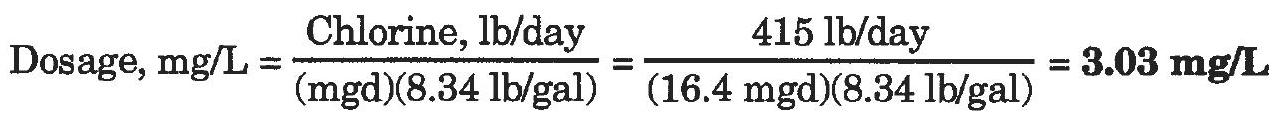
\includegraphics[max width=\textwidth]{2022_11_10_d6923b5a412978ed01fcg-36}

\begin{enumerate}
  \setcounter{enumi}{21}
  \item Answer: c. 59 gal sodium hypochlorite
\end{enumerate}

First, find the initial amount of water to be disinfected, $10 \%$ capacity

$$
=(1.65 \mathrm{mil} \mathrm{gal})(10 \% \div 100 \%)=0.165 \mathrm{mil} \mathrm{gal}
$$

Next, determine the number of pounds of chlorine needed by using the "pounds" equation.

Sodium hypochlorite, $\mathrm{lb}=\frac{(\mathrm{mil} \text { gal })(\text { Dosage, } \mathrm{mg} / \mathrm{L})(8.34 \mathrm{lb} / \mathrm{gal})}{\text { (\% Available chlorine) }(100 \%)}$

Sodium hypochlorite, $1 \mathrm{~b}=\frac{(0.165 \mathrm{mil} \mathrm{gal})(50.0 \mathrm{mg} / \mathrm{L})(8.34 \mathrm{lb} / \mathrm{gal})(100 \%)}{(11.8 \%)}$

Lastly, convert the pounds of sodium hypochlorite to gallons by dividing by 9.84 lb/gal.

Sodium hypochlorite, gal $=583.1 \mathrm{lb} \div 9.84 \mathrm{lb} / \mathrm{gal}=59.26$, round to $59 \mathrm{gal}$

\begin{enumerate}
  \setcounter{enumi}{22}
  \item Answer: c. $11.9 \mathrm{lb}$ calcium hypochlorite
\end{enumerate}

First, convert 24 in. to feet: 24 in. $\div 12$ in. per foot $=2 \mathrm{ft}$

Next, find the volume of the pipe in gallons using the following formula:

Equation: Pipe volume, gal $=(0.785)(\text { Diameter, } \mathrm{ft})^{2}($ Length, $\mathrm{ft})\left(7.48 \mathrm{gal} / \mathrm{ft}^{3}\right)$

Pipe volume, gal $=(0.785)(2.0 \mathrm{ft})(2.0 \mathrm{ft})(781 \mathrm{ft})\left(7.48 \mathrm{gal} / \mathrm{ft}^{3}\right)=18,344 \mathrm{gal}$

Next, find the number of million gallons (mil gal).

mil gal $=(18,344 \mathrm{gal})(1 \mathrm{M} \div 1,000,000)=0.018344 \mathrm{mil} \mathrm{gal}$

Then use the "pounds" equation:

Calcium hypochlorite, $\mathrm{lb}=\frac{(\mathrm{mil} \text { gal })(\text { Dosage, } \mathrm{mg} / \mathrm{L})(8.34 \mathrm{lb} / \mathrm{gal})}{(\% \text { Available chlorine })(100 \%)}$

Calcium hypochlorite, $\mathrm{lb}=\frac{(0.018344 \mathrm{mil} \mathrm{gal})(50.0 \mathrm{mg} / \mathrm{L})(8.34 \mathrm{lb} / \mathrm{gal})}{(64.3 \%)(100 \%)}=\mathbf{1 1 . 9} \mathbf{1 b}$ 24. Answer: d. $26.0 \mathrm{lb} /$ day of chlorine

First, convert the pumping rate to million gallons per day (mgd).

Equation: $\mathrm{mgd}=\frac{(\text { Pumping rate, } g p m)(1,440 \mathrm{~min} / \text { day })}{1,000,000}$

Substitute known values and solve: $\mathrm{mgd}=\frac{(428 \mathrm{gpm})(1,440 \mathrm{~min} / \mathrm{day})}{1,000,000}=0.61632 \mathrm{mgd}$

Next, find the total chlorine dose required.

Total chlorine dose, $\mathrm{mg} / \mathrm{L}=1.20 \mathrm{mg} / \mathrm{L}$ required $+3.85 \mathrm{mg} / \mathrm{L}$ demand $=5.05 \mathrm{mg} / \mathrm{L}$

Next, use the "pounds" equation to solve the problem.

Chlorine, lb/day $=(\mathrm{mgd})($ Dosage, $\mathrm{mg} / \mathrm{L})(8.34 \mathrm{lb} / \mathrm{gal})$

$=(0.61632 \mathrm{mgd})(5.05 \mathrm{mg} / \mathrm{L})(8.34 \mathrm{lb} / \mathrm{gal})$

$=25.958 \mathrm{lb} /$ day, round to $26.0 \mathrm{lb} / \mathrm{day}$

\begin{enumerate}
  \setcounter{enumi}{24}
  \item Answer: b. $74.4 \mathrm{cfs}$
\end{enumerate}

Equation: Number of $\mathrm{cfs}=\frac{(\mathrm{mgd})(1,000,000 \mathrm{gal})\left(1 \mathrm{ft}^{3}\right)(1 \mathrm{day})(1 \mathrm{~min})}{(1 \mathrm{mil} \mathrm{gal})(7.48 \mathrm{gal})(1,440 \mathrm{~min})(60 \mathrm{sec})}$

or: Number of $\mathrm{cfs}=\frac{(\mathrm{mgd})(1,000,000 \mathrm{gal})\left(1 \mathrm{ft}^{3}\right)(1 \mathrm{day})}{(1 \mathrm{mil} \mathrm{gal})(7.48 \mathrm{gal})(86,400 \mathrm{sec})}$

Substitute known values and solve.

Number of $\mathrm{cfs}=\frac{(48.1 \mathrm{mgd})(1,000,000 \mathrm{gal})\left(1 \mathrm{ft}^{3}\right)(1 \mathrm{day})}{(1 \mathrm{mil} \mathrm{gal})(7.48 \mathrm{gal})(86,400 \mathrm{sec})}=\mathbf{7 4 . 4} \mathrm{cfs}$

\begin{enumerate}
  \setcounter{enumi}{25}
  \item Answer: c. $11.6 \mathrm{~L} / \mathrm{s}$
\end{enumerate}

Equation: Flow, L/s $=\frac{(F l o w, g p m)(3.785 \mathrm{~L} / \mathrm{gal})}{60 \mathrm{sec} / \mathrm{min}}$

Flow, $\mathrm{L} / \mathrm{s}=\frac{(184 \mathrm{gpm})(3.785 \text { Liters } / \mathrm{gal})}{60 \mathrm{sec} / \mathrm{min}}=11.6 \mathrm{~L} / \mathrm{s}$

\begin{enumerate}
  \setcounter{enumi}{26}
  \item Answer: c. $1.02 \mathrm{ntu}$
\end{enumerate}

\begin{tabular}{|c|c|c|c|c|c|c|}
\hline
1 & 2 & 3 & 4 & 5 & 6 & 7 \\
\hline
$1.08 \mathrm{ntu}$ & $0.98 \mathrm{ntu}$ & $0.94 \mathrm{ntu}$ & $0.88 \mathrm{ntu}$ & $0.96 \mathrm{ntu}$ & $1.03 \mathrm{ntu}$ & $1.25 \mathrm{ntu}$ \\
\hline
\end{tabular}

First add all seven measurements:

$1.08+0.98+0.94+0.88+0.96+1.03+1.25=7.12 \mathrm{ntu}$

Equation: Average $=\frac{\text { Sum of measurements }}{\text { Number of measurements }}$

Average sedimentation basin $\mathrm{ntu}=\frac{7.12 \mathrm{mg} / \mathrm{L}}{7}=1.017 \mathrm{ntu}$, round to $1.02 \mathrm{ntu}$

\begin{enumerate}
  \setcounter{enumi}{27}
  \item Answer: a. 410
\end{enumerate}

Equation: $100 \%$ Number $=\frac{\text { (Number given })(100 \%)}{\text { Percent of given number }}$

$100 \%$ Number $=\frac{(288)(100 \%)}{70.3 \%}=409.67$, round to 410 29. Answer: d. $99 \%$ Fe removal efficiency

Equation: Percent Fe removal efficiency $=\frac{(\text { In }-\text { Out })(100 \%)}{\text { In }}$

Percent Fe removal efficiency $=\frac{(0.81-0.01)(100 \%)}{0.81}=99 \%$ Fe removal efficiency

\begin{enumerate}
  \setcounter{enumi}{29}
  \item Answer: a. $3.27 \%$ soda ash slurry
\end{enumerate}

Equation: Percent soda ash slurry $=\frac{\text { (Soda ash, } \mathrm{lb})(100 \%)}{\text { Soda ash, } \mathrm{lb}+(8.34 \mathrm{lb} / \mathrm{gal})(\text { Water, gal) }}$

Substitute known values and solve.

$$
\begin{aligned}
\text { Percent soda ash slurry } &=\frac{(28.2 \mathrm{lb})(100 \%)}{28.2 \mathrm{lb}+(8.34 \mathrm{lb} / \mathrm{gal})(100.0 \mathrm{gal})} \\
&=\frac{(28.2 \mathrm{lb})(100 \%)}{28.2 \mathrm{lb}+834 \mathrm{lb}}=\frac{(28.2 \mathrm{lb})(100 \%)}{862.2 \mathrm{lb}} \\
&=\mathbf{3 . 2 7 \%} \text { soda ash slurry }
\end{aligned}
$$

\begin{enumerate}
  \setcounter{enumi}{30}
  \item Answer: d. $11,100 \mathrm{ft}^{2}$
\end{enumerate}

First, find the square footage of the wall area.

Equation: Wall area, $\mathrm{ft}^{2}=($ Diameter, $\mathrm{ft})(\pi)($ Height, $\mathrm{ft})$; where $\pi$ equals $3.14$

Wall area, $\mathrm{ft}^{2}=(80.1 \mathrm{ft})(3.14)(24.0 \mathrm{ft})=6,036 \mathrm{ft}^{2}$

Next, find the area of the top. Note: There is no bottom exterior area.

Top area, $\mathrm{ft}^{2}=(0.785)(\text { Diameter, } \mathrm{ft})^{2}=(0.785)(80.1 \mathrm{ft})(80.1 \mathrm{ft})=5,037 \mathrm{ft}^{2}$

Total exterior surface area of tank, $\mathrm{ft}^{2}=6,036 \mathrm{ft}^{2}+5,037 \mathrm{ft}^{2}$

$=11,073 \mathrm{ft}^{2}$, round to $11,100 \mathrm{ft}^{2}$

\begin{enumerate}
  \setcounter{enumi}{31}
  \item Answer: c. $99,800 \mathrm{gal}$
\end{enumerate}

First, convert miles to feet:

Number of miles $=(1.43 \mathrm{miles})(5,280 \mathrm{ft} / \mathrm{mile})=7,550.4 \mathrm{ft}$

Next, convert $18.0$ inches to feet:

Number of $\mathrm{ft}=18.0$ inches $/ 12$ inches per foot $=1.50 \mathrm{ft}$

Substitute known values and solve.

Equation: Volume, gal $=(0.785)(\text { Diameter, } \mathrm{ft})^{2}($ Length, $\mathrm{ft})\left(7.48 \mathrm{gal}^{\mathrm{ft}} \mathrm{ft}^{3}\right)$

Volume, gal $=(0.785)(1.50 \mathrm{ft})(1.50 \mathrm{ft})(7,550.4 \mathrm{ft})\left(7.48 \mathrm{gal} / \mathrm{ft}^{3}\right)$

$=99,752$ gal, round to $99,800 \mathrm{gal}$

\begin{enumerate}
  \setcounter{enumi}{32}
  \item Answer: b. $17.8 \mathrm{hr}$
\end{enumerate}

First, find the diameter: Diameter, $\mathrm{ft}=2$ (radius) $=2(60.0 \mathrm{ft})=120 \mathrm{ft}$

Then, determine the volume of water in the storage tank.

Equation: Volume, gal $=(0.785)(\text { Diameter, } \mathrm{ft})^{2}($ Depth, $\mathrm{ft})\left(7.48 \mathrm{gal} / \mathrm{ft}^{3}\right)$

Average Tank Volume, gal $=(0.785)(120 \mathrm{ft})(120 \mathrm{ft})(25.5 \mathrm{ft})\left(7.48 \mathrm{gal}^{2} / \mathrm{ft}^{3}\right)$

$$
=2,156,125 \mathrm{gal}
$$

Next, convert mgd to gallons per day.

Flow through tank, gal/day $=(2.91 \mathrm{mgd})(1,000,000 \mathrm{gal})=2,910,000 \mathrm{gal} /$ day

Next, solve for the detention.

Equation: Detention time, $\mathrm{hr}=[($ Tank Volume $)(24 \mathrm{hr} /$ day $)] \div(\mathrm{Flow}$, gal/day) Substitute known values and solve:

Detention time, $\mathrm{hr}=[(2,156,125 \mathrm{gal})(24 \mathrm{hr} /$ day $)] \div(2,910,000 \mathrm{gal} / \mathrm{day})=17.8 \mathrm{hr}$

\begin{enumerate}
  \setcounter{enumi}{33}
  \item Answer: d. $58 \mathrm{psi}$
\end{enumerate}

Equation: Pressure Head, $\mathrm{ft}=($ Pressure, $\mathrm{psi})(2.31 \mathrm{ft} / \mathrm{psi})$

Rearrange to solve for pressure in psi:

Pressure, psi $=($ Pressure head, $\mathrm{ft}) \div(2.31 \mathrm{ft} / \mathrm{psi})$

Pressure, $\mathrm{psi}=134 \mathrm{ft} \div 2.31 \mathrm{ft} / \mathrm{psi}=58 \mathrm{psi}$

\begin{enumerate}
  \setcounter{enumi}{34}
  \item Answer: a. $820 \mathrm{gal}$
\end{enumerate}

First, convert the flow in $\mathrm{ft}^{3} / \mathrm{min}$ to gallons per minute (gpm).

$\mathrm{gpm}=\left(5.5 \mathrm{ft}^{3} / \mathrm{min}\right)\left(7.48 \mathrm{gal} / \mathrm{ft}^{3}\right)=41.14 \mathrm{gpm}$

Then determine the number of gallons that flowed through the fire hydrant.

Gallons $=(41.14 \mathrm{gpm})(20 \mathrm{~min})=822.8 \mathrm{gal}$, round to $820 \mathrm{gal}$

\begin{enumerate}
  \setcounter{enumi}{35}
  \item Answer: b. $1.19 \mathrm{~g} / \mathrm{cm}^{3}$
\end{enumerate}

First, convert the number of pounds to grams.

Know from conversion tables that 1 pound $=454$ grams and 1 liter $=1000.027 \mathrm{~cm}^{3}$

Number of grams $=(\mathrm{Number}$ of $\mathrm{lb})(454 \mathrm{~g} / \mathrm{lb})$

Number of grams $=(8.25 \mathrm{lb})(454 \mathrm{~g} / \mathrm{lb})=3,745.5 \mathrm{~g}$

Number of $\mathrm{cm}^{3}=\left(1000.027 \mathrm{~cm}^{3} / 1 \mathrm{~L}\right)(3.150 \mathrm{~L})=3,150.085 \mathrm{~cm}^{3}$

Equation: Density = Mass/Volume

Density $=3,745.5 \mathrm{~g} / 3,150.085 \mathrm{~cm}^{3}=1.19 \mathrm{~g} / \mathrm{cm}^{3}$

\begin{enumerate}
  \setcounter{enumi}{36}
  \item Answer: b. $98.6 \%$ meter efficiency
\end{enumerate}

First, convert cubic feet to gallons.

Number of gal $=\left(245.7 \mathrm{ft}^{3}\right)\left(7.48 \mathrm{gal} / \mathrm{ft}^{3}\right)=1,837.836 \mathrm{gal}$

Equation: Meter accuracy, $\%=\frac{(\text { Meter reading, gal })(100 \%)}{\text { Actual volume, gal }}$

Meter accuracy, $\%=\frac{(1,837.836 \mathrm{gal})(100 \%)}{1,863 \mathrm{gal}}=98.6 \%$ meter efficiency

\begin{enumerate}
  \setcounter{enumi}{37}
  \item Answer: c. $3.3 \mathrm{mg} / \mathrm{L}$
\end{enumerate}

Equation: $\mathrm{lb} / \mathrm{day}=(\mathrm{mgd})($ Dosage, $\mathrm{mg} / \mathrm{L})(8.34 \mathrm{lb} /$ day $)$

Rearrange the equation and solve for dosage.

Dosage, $\mathrm{mg} / \mathrm{L}=\frac{\mathrm{lb} / \text { day }}{(\mathrm{mgd})(8.34 \mathrm{lb} / \mathrm{gal})}=\frac{320 \mathrm{lb} / \mathrm{day}}{(11.6 \mathrm{mgd})(8.34 \mathrm{lb} / \mathrm{gal})}$

$=3.308 \mathrm{mg} / \mathrm{L}$, round to $3.3 \mathrm{mg} / \mathbf{L}$

\begin{enumerate}
  \setcounter{enumi}{38}
  \item Answer: a. 678 gal of sodium hypochlorite
\end{enumerate}

First, determine the number of pounds of chlorine needed by using the "pounds" equation.

Equation: Sodium hypochlorite, $\mathrm{lb}=(\mathrm{mil} \mathrm{gal})($ Dosage, $\mathrm{mg} / \mathrm{L})(8.34 \mathrm{lb} / \mathrm{gal})$ Chlorine, $\mathrm{lb}=(1.75 \mathrm{mil} \mathrm{gal})(50.0 \mathrm{mg} / \mathrm{L})(8.34 \mathrm{lb} / \mathrm{gal})=729.75 \mathrm{lb}$

Next, find the number of gallons of sodium hypochlorite.

Equation: Sodium hypochlorite, gal $=\frac{(\text { Chlorine, } \mathrm{lb})(100 \%)}{(\mathrm{lb} / \text { gal })(\% \text { Solution })}$

Substitute known values and solve.

Sodium hypochlorite, gal $=\frac{\left(729.75 \mathrm{lb} \text { of } \mathrm{Cl}_{2}\right)(100 \%)}{(8.97 \mathrm{lb} / \mathrm{gal})(12.0 \%)}=677.95 \mathrm{gal}$, round to $678 \mathrm{gal}$

\begin{enumerate}
  \setcounter{enumi}{39}
  \item Answer: d. $54 \mathrm{mg} / \mathrm{L}$ chlorine
\end{enumerate}

First, convert the diameter of the pipeline from inches to feet.

Number of feet $=24.0$ in. $\div 12$ in. $/ \mathrm{ft}=2.0 \mathrm{ft}$

Next, find the number of gallons by determining the volume of the pipeline.

Equation: Volume of pipe, gal $=(0.785)$ (Diameter, $\mathrm{ft})^{2}($ Length, $\mathrm{ft})$

Volume of pipe, gal $=(0.785)(2.0 \mathrm{ft})(2.0 \mathrm{ft})(427 \mathrm{ft})\left(7.48 \mathrm{gal} / \mathrm{ft}^{3}\right)=10,029 \mathrm{gal}$

Then convert number of gallons to mil gal.

Number of mil gal $=10,029 \mathrm{gal} \div 1,000,000=0.010029 \mathrm{mil} \mathrm{gal}$

Finally, calculate the dosage by rearranging the "pounds" equation.

Calcium hypochlorite, lb/day $=\frac{(\mathrm{mgd})(\text { Dosage, } \mathrm{mg} / \mathrm{L})(8.34 \mathrm{lb} / \mathrm{gal})(100 \%)}{\text { Percent available chlorine }}$

Rearrange the equation and drop the day on each side of the equation as it is not needed.

Dosage, $\mathrm{mg} / \mathrm{L}=\frac{(\text { Calcium hypochlorite, } \mathrm{lb})(65.0 \% \text { Available chlorine })}{\text { (mil gal })(8.34 \mathrm{lb} / \mathrm{gal})(100 \% \text { calcium hypochlorite })}$

$$
\begin{aligned}
&=\frac{(7.0)(65.0 \%)}{(0.010029)(8.34)(100 \%)} \\
&=54.4 \mathrm{mg} / \mathrm{L}, \text { round to } 54 \mathrm{mg} / \mathrm{L}
\end{aligned}
$$

\begin{enumerate}
  \setcounter{enumi}{40}
  \item Answer: c. $7.4 \mathrm{mg} / \mathrm{L}$ sodium hypochlorite
\end{enumerate}

First, convert the production rate of the well pump to mgd.

Equation: mgd $=\frac{\text { (Pumping rate) }(1,440 \mathrm{~min} / \text { day })}{1,000,000}$

$\mathrm{mgd}=\frac{(260 \mathrm{gpm})(1,440 \mathrm{~min} / \mathrm{day})}{1,000,000 \mathrm{mil} \mathrm{gal}}=0.3744 \mathrm{mgd}$

Second, convert liters/day to gallons/day.

Number of gal $=\frac{95 \text { Liters } / \text { day }}{3.785 \text { Liters } / \text { gal }}=25.1 \mathrm{gal} /$ day

Next, calculate the chlorine usage in pounds per day. Equation:

Chlorine usage, lb/day

$$
\begin{aligned}
&=\frac{(\text { Hypochlorinator flow, gal/day })\left(\% \mathrm{Cl}_{2} \text { in hypochlorite solution }\right)(8.95 \mathrm{lb} / \mathrm{gal})}{100 \%} \\
&=\frac{(25.1 \mathrm{gal} / \mathrm{day})(10.3 \%)(8.95 \mathrm{lb} / \mathrm{gal})}{100 \%}=23.14 \mathrm{lb} / \mathrm{day}
\end{aligned}
$$

Lastly, calculate the chlorine dosage using the "pounds" equation. Sodium hypochlorite, lb/day $=[(\mathrm{mgd})($ Dosage, $\mathrm{mg} / \mathrm{L})(8.34 \mathrm{lb} / \mathrm{gal})]$

Rearrange the equation to solve for dosage.

Equation: Dosage, $\mathrm{mg} / \mathrm{L}=\frac{\text { Sodium hypochlorite, } \mathrm{lb} / \text { day }}{(\mathrm{mgd})(8.34 \mathrm{lb} / \mathrm{gal})}$

Dosage, $\mathrm{mg} / \mathrm{L}=\frac{23.14}{(0.3744)(8.34)}=7.4 \mathrm{mg} / \mathrm{L}$ sodium hypochlorite

\begin{enumerate}
  \setcounter{enumi}{41}
  \item Answer: a. $10.5 \mathrm{lb} /$ day of chlorine
\end{enumerate}

First, convert the pumping rate to mgd.

Equation: $m g d=\frac{\text { (pumping rate, gpm })(1,440 \mathrm{~min} / \text { day })}{1,000,000}$

Substitute known values and solve:

$\mathrm{mgd}=\frac{(208 \mathrm{gpm})(1,440 \mathrm{~min} / \text { day })}{1,000,000}=0.29952 \mathrm{mgd}$

Next determine the total chlorine dosage required.

Total chlorine, $\mathrm{mg} / \mathrm{L}=$ Chlorine demand, $\mathrm{mg} / \mathrm{L}+$ chlorine residual, $\mathrm{mg} / \mathrm{L}$

Total chlorine, $\mathrm{mg} / \mathrm{L}=2.45 \mathrm{mg} / \mathrm{L}+1.75 \mathrm{mg} / \mathrm{L}=4.20 \mathrm{mg} / \mathrm{L}$

Next, use the "pounds" equation to solve the problem.

Equation: Chlorine, lb/day $=(\mathrm{mgd})($ Dosage, $\mathrm{mg} / \mathrm{L})(8.34 \mathrm{lb} / \mathrm{gal})$

Chlorine, lb/day $=(0.29952 \mathrm{mgd})(4.20 \mathrm{mg} / \mathrm{L})(8.34 \mathrm{lb} / \mathrm{gal})=\mathbf{1 0 . 5} \mathrm{lb} /$ day chlorine

\begin{enumerate}
  \setcounter{enumi}{42}
  \item Answer: b. $910 \mathrm{gpm}$
\end{enumerate}

Know: $1 \mathrm{hp}=33,000 \mathrm{ft}-\mathrm{lb} / \mathrm{min}$

Convert $15 \mathrm{hp}$ to $\mathrm{ft}-\mathrm{lb} / \mathrm{min}: 15 \times 33,000=495,000 \mathrm{ft}-\mathrm{lb} / \mathrm{min}$

Solve for the unknown value, $x$ :

$(65)(x \mathrm{lb} / \mathrm{min})=495,000 \mathrm{ft}-\mathrm{lb} / \mathrm{min}$

$x \mathrm{lb} / \mathrm{min}=495,000 \mathrm{ft}-\mathrm{lb} / \mathrm{min} \div 65=7,615 \mathrm{lb} / \mathrm{min}$

Now express this maximum pumping rate in gallons per minute

$7,615 \mathrm{lb} / \mathrm{min} \div 8.34 \mathrm{lb} / \mathrm{gal}=913.70 \mathrm{gpm}$, round to $910 \mathrm{gpm}$

\begin{enumerate}
  \setcounter{enumi}{43}
  \item Answer: 128 gpcd
\end{enumerate}

First, convert $2.98 \mathrm{mgd}$ to mil gal.

Number of gallons $=2.98 \mathrm{mgd} \times 1,000,000 \mathrm{mil} \mathrm{gal}=2,980,000 \mathrm{gal}$

Equation:

Gallons per capita per day $(\mathrm{gpcd})=$ Volume gal/day $\div$ Population served/day

gpcd $=2,980,000 \mathrm{gal} /$ day $\div 23,210$ capita/day $=128 \mathrm{gpcd}$

\section{Answers to Math Questions for Water Distribution Operators Levels Ill \& IV}
\begin{enumerate}
  \item Answer: d. $1.4 \mathrm{ft} / \mathrm{sec}$
\end{enumerate}

First, convert gpm to cubic feet per second (cfs).

Number of $\mathrm{cfs}=\frac{122 \mathrm{gpm}}{\left(7.48 \mathrm{gal} / \mathrm{ft}^{2}\right)(60 \mathrm{sec} / \mathrm{min})}=0.2718 \mathrm{cfs}$

Next, convert the diameter from inches to feet.

Number of $\mathrm{ft}=(6.0-\mathrm{in})(1 \mathrm{ft} / 12$-in $)=0.50 \mathrm{ft}$

Equation: Flow, $\mathrm{cfs}=\left(\right.$ Area, $\left.\mathrm{ft}^{2}\right)($ Velocity, $\mathrm{ft} / \mathrm{sec})$; where the Area $=(0.785)(\text { Diameter })^{2}$

$0.2718 \mathrm{cfs}=(0.785)(0.50 \mathrm{ft})(0.50 \mathrm{ft})(\mathrm{Flow}, \mathrm{ft} / \mathrm{sec})$

Rearrange and solve for the flow in $\mathrm{ft} / \mathrm{sec}$.

Flow, $\mathrm{ft} / \mathrm{sec}=\frac{0.2718 \mathrm{cfs}}{(0.785)(0.50 \mathrm{ft})(0.50 \mathrm{ft})}=1.38$, round to $1.4 \mathrm{ft} / \mathrm{sec}$

\begin{enumerate}
  \setcounter{enumi}{1}
  \item Answer: b. $1,200 \mathrm{lb}$
\end{enumerate}

Equation: Pressure $=\frac{\text { Force, } \mathrm{lb}}{\text { Area, } \mathrm{ft}^{2}}$ for pressure on the small cylinder.

First convert 10 -inches to $\mathrm{ft}:(10 \mathrm{in})(1 \mathrm{ft} / 12 \mathrm{in})=0.833 \mathrm{ft}$

Pressure $=\frac{130 \mathrm{lb}}{(0.785)(0.833 \mathrm{ft})(0.833 \mathrm{ft})}=238.66 \mathrm{lb} / \mathrm{ft}^{2}$

Next, calculate the total force on the large cylinder.

Equation: Total force $=($ Pressure $)($ Area $)$

Total force $=\left(238.66 \mathrm{lb} / \mathrm{ft}^{2}\right)(0.785)(2.5 \mathrm{ft})(2.5 \mathrm{ft})=1,170.926 \mathrm{lb}$, round to $1,200 \mathrm{lb}$

\begin{enumerate}
  \setcounter{enumi}{2}
  \item Answer: c. $50 \mathrm{mg} / \mathrm{L}$
\end{enumerate}

First, find the number of feet in $2.45$ miles

Length in $\mathrm{ft}=(5,280 \mathrm{ft} / \mathrm{mile})(2.45 \mathrm{miles})=12,936 \mathrm{ft}$

Next, find the volume in cubic feet $\left(\mathrm{ft}^{3}\right)$ for the pipe.

Equation: Volume, $\mathrm{ft}^{3}=(0.785)(\text { Diameter, } \mathrm{ft})^{2}($ Length, $\mathrm{ft})$

Volume, $\mathrm{ft}^{3}=(0.785)(2.0 \mathrm{ft})(2.0 \mathrm{ft})(12,936 \mathrm{ft})=40,619.04 \mathrm{ft}^{3}$

Then, determine the number of gallons.

Number of $\mathrm{gal}=\left(40,619.04 \mathrm{ft}^{3}\right)\left(7.48 \mathrm{gal} / \mathrm{ft}^{3}\right)=303,830.42 \mathrm{gal}$

Convert the number of gallons to million gallons (mil gal).

mil gal $=\frac{303,830.42 \mathrm{gal}}{1,000,000}=0.30383 \mathrm{mil} \mathrm{gal}$

Lastly, find the dosage in $\mathrm{mg} / \mathrm{L}$.

Dosage, $\mathrm{mg} / \mathrm{L}=\frac{\mathrm{lb} \text { of Chlorine }}{(\mathrm{mil} \mathrm{gal})(8.34 \mathrm{lb} / \mathrm{gal})}=\frac{126.9}{(0.30383)(8.34)}$

$=50.08 \mathrm{mg} / \mathrm{L}$, round to $50 \mathrm{mg} / \mathrm{L}$ 4. Answer: d. $310 \mathrm{mhp}$

$$
\begin{aligned}
\text { Equation: Motor hp } &=\frac{\text { whp }}{(\text { Motor effic. })(\text { Pump effic. })} \\
\text { Motor hp } &=\frac{200 \text { whp }}{(88 \% / 100 \% \text { Motor effic. })(74 \% / 100 \% \text { Pump effic. })} \\
&=\frac{(200 \mathrm{whp})}{(0.88 \text { Motor effic. })(0.74 \text { Pump effic. })}=307 \mathrm{mhp}, \text { round to } 310 \mathbf{~ m h p}
\end{aligned}
$$

\begin{enumerate}
  \setcounter{enumi}{4}
  \item Answer: c. 26 bhp
\end{enumerate}

Solution: bhp $=\frac{(\text { Bowl head, ft })(\text { Capacity, gpm })}{(3960)(\text { Bowl efficiency, \%/100\%) }}$

$$
\text { bhp }=\frac{(215 \mathrm{ft})(385 \mathrm{gpm})}{(3960)(81 \% / 100 \%)}=25.8 \mathrm{bhp} \text {, round to } 2 \mathbf{6 h p}
$$

\begin{enumerate}
  \setcounter{enumi}{5}
  \item Answer: c. $2.3 \mathrm{ft} / \mathrm{sec}$
\end{enumerate}

Flow in 4.0-inch pipe equals the flow in the 3.0-inch pipe as the flow must remain constant: $\mathrm{Q}_{1}=\mathrm{Q}_{2}$

Equation: $($ Area 1 $)($ Velocity 1) $=($ Area 2) $($ Velocity 2)

First, find the diameter for the 3.0-inch and 4.0-inch pipes:

Diameter for 3.0-inch $=(3.0$-inch $)(1 \mathrm{ft} / 12$-in $)=0.25 \mathrm{ft}$

Diameter for 4.0-inch $=(4.0$-inch $)(1 \mathrm{ft} / 12$-in $)=0.333 \mathrm{ft}$

Then determine the areas of each size pipe: Area $=(0.785)(\text { Diameter, } \mathrm{ft})^{2}$

Area $1(3.0$-in $)=(0.785)(0.25 \mathrm{ft})(0.25 \mathrm{ft})=0.049 \mathrm{ft}^{2}$

Area $2(4.0$-in $)=(0.785)(0.333 \mathrm{ft})(0.333 \mathrm{ft})=0.087 \mathrm{ft}^{2}$

Lastly, substitute areas calculated and known velocity in $4.0$-inch pipe.

$\left(0.049 \mathrm{ft}^{2}\right)(x, \mathrm{ft} / \mathrm{sec})=\left(0.087 \mathrm{ft}^{2}\right)(1.3 \mathrm{ft} / \mathrm{sec})$

Solve for $x$ :

$$
x, \mathrm{ft} / \mathrm{sec}=\frac{\left(0.087 \mathrm{ft}^{2}\right)(1.3 \mathrm{ft} / \mathrm{sec})}{\left(0.049 \mathrm{ft}^{2}\right)}=2.308 \mathrm{ft} / \mathrm{sec}, \text { round to } 2.3 \mathrm{ft} / \mathrm{sec}
$$

\begin{enumerate}
  \setcounter{enumi}{6}
  \item Answer: b. $3,500 \mathrm{gpm}$
\end{enumerate}

First, find the water production during the 18-hour interval.

Gallons of water treated in 18-hr interval =

$$
[(4.75 \mathrm{mgd})(1,000,000)(18 \mathrm{hrs})] \div 24 \mathrm{hrs}=3,562,500 \mathrm{gal}
$$

Next, find the gallons contained in the $2.3 \mathrm{ft}$ drop in water level.

$$
\begin{aligned}
& \text { Volume, } \operatorname{tank}=(0.785)(\text { Diameter, } \mathrm{ft})^{2}(\text { Height }) \\
& \text { Volume of } 2.3 \mathrm{ft}, 120 \mathrm{ft} \text { diameter tank }=(0.785)(120 \mathrm{ft})(120 \mathrm{ft})(2.3 \mathrm{ft})\left(7.48 \mathrm{gal} / \mathrm{ft}^{3}\right) \\
& =194,474 \mathrm{gal}
\end{aligned}
$$

Production plus the loss in level is the amount the discharge pump had to send into the distribution system, but first find the number of minutes in $18 \mathrm{hrs}$.

$(18 \mathrm{hrs})(60 \mathrm{~min} / \mathrm{hr})=1,080 \mathrm{~min}$

Then determine total gallons discharge pump moved.

Total gal discharge pump moved in $18 \mathrm{hrs}=3,562,500 \mathrm{gal}+194,474 \mathrm{gal}$

$$
=3,756,974 \mathrm{gal}
$$

Lastly, divide the number of gallons the discharge pump moved by the time in minutes.

Discharge pump, gpm $=3,756,974 \mathrm{gal} \div 1,080 \mathrm{~min}$

$$
=3,479 \mathrm{gpm} \text {, round to } 3,500 \mathrm{gpm}
$$

\begin{enumerate}
  \setcounter{enumi}{7}
  \item Answer: b. $0.4$ gal of sodium hypochlorite
\end{enumerate}

First, convert 1,000 gallons to million gallons:

Number of mil gal $=1,000$ gal $\div 1,000,000=0.001 \mathrm{mil}$ gal

Next determine the number of pounds of hypochlorite that are required using the "pounds" formula.

Equation: Sodium hypochlorite, $\mathrm{lb}=\frac{(\text { Dosage, } \mathrm{mg} / \mathrm{L})(\mathrm{mil} \text { gal })(8.34 \mathrm{lb} / \mathrm{gal})(100 \%)}{\text { Percent sodium hypochlorite }}$

Substitute known values and solve:

Sodium hypochlorite, $\mathrm{lb}=\frac{(50 \mathrm{mg} / \mathrm{L})(0.001 \mathrm{mil} \text { gal })(8.34 \mathrm{lb} / \mathrm{gal})(100 \%)}{12.5 \% \text { Sodium hypochlorite }}=3.736 \mathrm{lb}$

Lastly, determine the number of gallons of sodium hypochlorite by dividing by 9.34 lb/gal.

Sodium hypochlorite, gal $=3.736 \mathrm{lb} \div 9.34 \mathrm{lb} / \mathrm{gal}=\mathbf{0 . 4} \mathrm{gal}$

\begin{enumerate}
  \setcounter{enumi}{8}
  \item Answer: b. $9.0 \%$ final solution
\end{enumerate}

First, find the total volume that would result from mixing these two solutions:

Total Volume $=350 \mathrm{gal}+225 \mathrm{gal}=575 \mathrm{gal}$

Then write the equation:

$\left(\right.$ Concentration $\left._{1}\right)\left(\right.$ Volume $\left._{1}\right)+\left(\right.$ Concentration $\left._{2}\right)\left(\right.$ Volume $\left._{2}\right)=\left(\right.$ Concentration $\left._{3}\right)\left(\right.$ Volume $\left._{3}\right)$, or condensed as

$\mathrm{C}_{1} \mathrm{~V}_{1}+\mathrm{C}_{2} \mathrm{~V}_{2}=\mathrm{C}_{3} \mathrm{~V}_{3}$

where $\mathrm{C}_{1}$ and $\mathrm{C}_{2}=\%$ Concentration of the two solutions before being mixed, $\mathrm{V}_{1}$ and $\mathrm{V}_{2}=$ Volume of the two solutions before being mixed, and $\mathrm{C}_{3}$ and $\mathrm{V}_{3}=$ the resulting $\%$ Concentration and Volume, respectively.

Substituting:

$$
\begin{array}{r}
\frac{(11 \%)(350 \mathrm{gal})}{100 \%}+\frac{(5.8 \%)(225 \mathrm{gal})}{100 \%}=\frac{\mathrm{C}_{3}(575 \mathrm{gal})}{100 \%} \\
38.5 \mathrm{gal}+13.05 \mathrm{gal}=\frac{\mathrm{C}_{3}(575 \mathrm{gal})}{100 \%}
\end{array}
$$

Solving for $\mathrm{C}_{3}$ :

$$
\mathrm{C}_{3}=\frac{(38.5 \mathrm{gal}+13.05 \mathrm{gal})(100 \%)}{575 \mathrm{gal}}=\frac{(51.55 \mathrm{gal})(100 \%)}{575 \mathrm{gal}}=8.965, \text { round to } 9.0 \%
$$

\begin{enumerate}
  \setcounter{enumi}{9}
  \item Answer: c. $32 \mathrm{whp}$
\end{enumerate}

Equation: $w h p=\frac{(\text { Pump rate, gpm })(\text { Total head }, \mathrm{ft})(8.34 \mathrm{lb} / \mathrm{gal})}{33,000 \mathrm{ft}-\mathrm{lb} / \mathrm{min} / \mathrm{hp}}$

$$
w h p=\frac{(650 \mathrm{gpm})(195 \mathrm{ft})(8.34 \mathrm{lb} / \mathrm{gal})}{33,000 \mathrm{ft}-\mathrm{lb} / \mathrm{min} / \mathrm{hp}}=32 \mathrm{whp}
$$

\begin{enumerate}
  \setcounter{enumi}{10}
  \item Answer: a. $41.4 \%$
\end{enumerate}

Equation: Percent mixture

$\frac{(\text { Sol. 1-lb)(Percent Strength of Sol. 1) }}{100 \%}+\frac{(\text { Sol. 2-lb)(Percent Strength of Sol. 2) }}{100 \%}(100 \%)$

Sol. 1-lb + Sol. 2-lb

Where Sol. = solution

Substitute known values and solve:

Percent mixture $=\frac{\frac{(875 \mathrm{lb})(49.5 \%)}{100 \%}+\frac{(293 \mathrm{lb})(17.2 \%)}{100 \%}(100 \%)}{875 \mathrm{lb}+293 \mathrm{lb}}$

Reduce:

Percent mixture $=\frac{(433.125 \mathrm{lb}+50.396 \mathrm{lb})(100 \%)}{1,168 \mathrm{lb}}=\frac{(483.521 \mathrm{lb})(100 \%)}{1,168 \mathrm{lb}}$

$$
=41.397 \% \text {, round to } 41.4 \%
$$

\begin{enumerate}
  \setcounter{enumi}{11}
  \item Answer: d. $30 \mathrm{oz}$
\end{enumerate}

First, find the diameter in feet for both well casings.

Diameter for 12 -in. casing $=12$ in. $=1.00 \mathrm{ft}$

Diameter for 10 -in. casing $=10$ in. $\div 12$ in. $=0.833 \mathrm{ft}$

Then, find the length (in feet) of water in the casing.

Length of water-filled casing $=$ Depth of well - Depth of water to top of casing

Length of water-filled casing for 12 -in. diameter $=100 \mathrm{ft}-168.4 \mathrm{ft}=-68.4 \mathrm{ft}$; since it is negative there is no water in this section, and

Length of water-filled casing for 10 -in. diameter $=287 \mathrm{ft}-168.4 \mathrm{ft}=118.6 \mathrm{ft}$;

Next, determine the volume in gallons of water in the 10-in. casing using the equation:

Volume, in gal $=(0.785)(\text { Diameter, } f \mathrm{t})^{2}($ Length, $\mathrm{ft})\left(7.48 \mathrm{gal} / \mathrm{ft}^{3}\right)$

Vol., in gal for $10.0$-inch casing $=(0.785)(0.833 \mathrm{ft})(0.833 \mathrm{ft})(118.6 \mathrm{ft})\left(7.48 \mathrm{gal} / \mathrm{ft}^{3}\right)$

$$
=483 \mathrm{gal}
$$

Next, determine the number of mil gal.

mil gal $=(483 \mathrm{gal})(1 \mathrm{M} / 1,000,000)=0.000483 \mathrm{mil}$ gal.

Then, find the chlorine required.

Chlorine required $=$ Chlorine demand $+$ Chlorine residual.

Chlorine required $=4.7 \mathrm{mg} / \mathrm{L}+50.0 \mathrm{mg} / \mathrm{L}=54.7 \mathrm{mg} / \mathrm{L}$

Then, using the "pounds" equation, calculate the number of lb of sodium hypochlorite.

Sodium Hypochlorite, $\mathrm{lb}=\frac{(0.000483 \mathrm{mil} \mathrm{gal})(54.7 \mathrm{mg} / \mathrm{L})(8.34 \mathrm{lb} / \mathrm{gal})}{10.5 \% / 100 \% \text { available chlorine }}$

Sodium Hypochlorite, $\mathrm{lb}=2.0985 \mathrm{lb}$

Next, calculate the number of gallons of sodium hypochlorite required.

$2.0985 \mathrm{lb} \div 9.10 \mathrm{lb} / \mathrm{gal}=0.2306 \mathrm{gal}$

Lastly, convert to fluid ounces (oz):

Sodium hypochlorite, oz $=(0.2306 \mathrm{gal})(128 \mathrm{oz} / \mathrm{gal})=29.5 \mathrm{oz}$, round to $30 \mathrm{oz}$ 13. Answer: c. $\$ 1,156.15$

Equation: Cost, month $=(\mathrm{Hp})(\mathrm{hrs} /$ day $)(\#$ days $)(0.746 \mathrm{~kW} / \mathrm{Hp})(\mathrm{Cost} / \mathrm{kW}-\mathrm{hr})$

Substitute known values:

Cost, month $=(300 \mathrm{Hp})(4.2 \mathrm{hrs} /$ day $)(30$ days $)(0.746 \mathrm{~kW} / \mathrm{Hp})(\$ 0.041 / \mathrm{kW})$

Cost, month $=\$ 1,156.15$

\begin{enumerate}
  \setcounter{enumi}{13}
  \item Answer: d. $14.81 \mathrm{~mA}$
\end{enumerate}

Equation:

Current process reading $=\frac{\text { (Live signal, } \mathrm{mA}-4 \mathrm{~mA} \text { offset)(Maximum capacity) }}{16 \text { milliamp span }}$

Substitute known values and solve:

$16.55 \mathrm{ft}=\frac{\text { (Live signal, } \mathrm{mA}-4 \mathrm{~mA} \text { offset })(24.50 \mathrm{ft})}{16 \mathrm{~mA} \text { span }}$

Rearrange formula to solve for the current number of milliamps.

Live signal, $\mathrm{mA}-4 \mathrm{~mA}$ offset $=\frac{(16.55 \mathrm{ft})(16 \mathrm{~mA})}{24.50 \mathrm{ft}}$

Live signal, $\mathrm{mA}=\frac{(16.55 \mathrm{ft})(16 \mathrm{~mA})}{24.5 \mathrm{ft}}+4 \mathrm{~mA}$

Live signal, $\mathrm{mA}=10.808 \mathrm{~mA}+4 \mathrm{~mA}=14.808 \mathrm{~mA}$, round to $14.81 \mathrm{~mA}$

\begin{enumerate}
  \setcounter{enumi}{14}
  \item Answer: b. 21,900 gal
\end{enumerate}

First, convert the pipe diameters from inches to feet.

Large pipe, $\mathrm{ft}=14$-in. $\div 12$-in. $=1.167 \mathrm{ft}$

Small pipe, $\mathrm{ft}=10$-in. $\div 12$ in. $=0.833 \mathrm{ft}$

Next, convert the diameter in feet to the radius in feet by dividing by 2 .

Large pipe, $\mathrm{ft}=1.167 \mathrm{ft} \div 2=0.5835 \mathrm{ft}$

Small pipe, $\mathrm{ft}=0.833 \mathrm{ft} \div 2=0.4165 \mathrm{ft}$

Next determine the gallons in the 14-inch pipe and then the 10-inch pipe.

Equation: Number, gal $=2 / 3($ Length, $\mathrm{ft})(\pi)(\mathrm{r})^{2}\left(7.48 \mathrm{gal} / \mathrm{ft}^{3}\right)$; for large pipe

where $\mathrm{r}=$ radius and $\pi=3.14$

Number, gal $=2 / 3(3,270 \mathrm{ft})(3.14)(0.5835)^{2}\left(7.48 \mathrm{gal} / \mathrm{ft}^{3}\right)=17,432.89 \mathrm{gal}$

Number, gal $=1 / 3($ Length, $\mathrm{ft})(\pi)(\mathrm{r})^{2}\left(7.48 \mathrm{gal} / \mathrm{ft}^{3}\right)$

Number, gal $=1 / 3(3,270 \mathrm{ft})(3.14)(0.4165)^{2}\left(7.48 \mathrm{gal} / \mathrm{ft}^{3}\right)=4,441.07 \mathrm{gal}$

Lastly add the number of gallons for each pipe together.

Total number of gal $=17,432.89+4,441.07=21,873.96$, round to $21,900 \mathrm{gal}$

\begin{enumerate}
  \setcounter{enumi}{15}
  \item Answer: b. $290 \mathrm{lb}$
\end{enumerate}

Equation: \% Lime $=\frac{(x \mathrm{lb})(100 \%)}{x \mathrm{lb}+(\text { Water, gal })(8.34 \mathrm{lb} / \mathrm{gal})}$

$$
15 \% \text { Lime }=\frac{(x \mathrm{lb})(100 \%)}{x \mathrm{lb}+(200 \mathrm{gal})(8.34 \mathrm{lb} / \mathrm{gal})}
$$

Multiply both sides of the equation by $\{x \mathrm{lb}+(200 \mathrm{gal})(8.34 \mathrm{lb} / \mathrm{gal})\}$. This leaves the following: $15 \%$ Lime $\{x \mathrm{lb}+(200 \mathrm{gal})(8.34 \mathrm{lb} / \mathrm{gal})\}=(x \mathrm{lb})(100 \%)$

Complete the multiplication.

$15 x \%, \mathrm{lb}+25,020 \%, \mathrm{lb}=100 x \%, \mathrm{lb}$

Subtract $15 x \%, \mathrm{lb}$ from both sides of the equation.

$25,020 \%, \mathrm{lb}=85 x \%, \mathrm{lb}$

Lastly, divide both sides of the equation by $85 \%$.

$x=294.35 \mathrm{lb}$, round to $\mathbf{2 9 0} \mathbf{~ l b}$

\begin{enumerate}
  \setcounter{enumi}{16}
  \item Answer: d. $1,540,000 \mathrm{gal}$
\end{enumerate}

Equation: Volume, gal $=\frac{\left(\mathrm{b}_{1}+\mathrm{b}_{2}\right)(\text { Height, } \mathrm{ft})(\text { Length, } \mathrm{ft})\left(7.48 \mathrm{gal} / \mathrm{ft}^{3}\right)}{2}$

Volume, gal $=\frac{(5.85 \mathrm{ft}+10.6 \mathrm{ft})(4.10 \mathrm{ft})(6,091 \mathrm{ft})\left(7.48 \mathrm{gal} / \mathrm{ft}^{3}\right)}{2}$

Volume, gal $=\frac{(16.45 \mathrm{ft})(4.10 \mathrm{ft})(6,091 \mathrm{ft})\left(7.48 \mathrm{gal} / \mathrm{ft}^{3}\right)}{2}$

Reduce problem by dividing 2 into $4.10 \mathrm{ft}$

Volume, gal $=(16.45 \mathrm{ft})(2.05 \mathrm{ft})(6,091 \mathrm{ft})\left(7.48 \mathrm{gal} / \mathrm{ft}^{3}\right)$

Volume, gal $=1,536,420 \mathrm{gal}$, round to $1,540,000 \mathrm{gal}$

\begin{enumerate}
  \setcounter{enumi}{17}
  \item Answer: b. $4.16 \mathrm{hr}$
\end{enumerate}

First, determine the number of gallons in the clearwell, distribution pipe, and storage tank.

Equation: Volume, gal $=($ Length, $\mathrm{ft})($ Width, $\mathrm{ft})($ Depth, $\mathrm{ft})\left(7.48 \mathrm{gal} / \mathrm{ft}^{3}\right)$

Clearwell volume, gal $=(308 \mathrm{ft})(118 \mathrm{ft})(12.85 \mathrm{ft})\left(7.48 \mathrm{gal} / \mathrm{ft}^{3}\right)=3,493,313 \mathrm{gal}$

Next, convert number of miles to feet.

Number of $\mathrm{ft}=(5,280 \mathrm{ft} / \mathrm{mi})(1.34$ miles $)=7,075.2 \mathrm{ft}$

Vol., gal in pipeline $=(0.785 \mathrm{ft})(2.00 \mathrm{ft})(2.00 \mathrm{ft})(7,075.2 \mathrm{ft})\left(7.48 \mathrm{gal} / \mathrm{ft}^{3}\right)$

$=166,177 \mathrm{gal}$

Volume, gal $=(0.785)(\text { Diameter, } \mathrm{ft})^{2}($ Height, $\mathrm{ft})\left(7.48 \mathrm{gal} / \mathrm{ft}^{3}\right)$

Vol., gal in tank $=(0.785)(99.8 \mathrm{ft})(99.8 \mathrm{ft})(26.48 \mathrm{ft})\left(7.48 \mathrm{gal} / \mathrm{ft}^{3}\right)=1,548,639 \mathrm{gal}$

Equation: Clearwell gal + Pipe gal + Tank gal = Total volume of gallons

$3,493,313 \mathrm{gal}+166,177 \mathrm{gal}+1,548,639 \mathrm{gal}=5,208,129 \mathrm{gal}$

Next, convert average mgd to gallons per hour (gph).

$(30.02$ mgd $\div 24$ hours $)(1,000,000)=1,250,833$ gph

Now solve for detention time.

Equation: Detention time, $\mathrm{hr}=$ Volume, gal $\div$ Flow rate, gph

Detention time, $\mathrm{hr}=5,208,129 \mathrm{gal} \div 1,250,833 \mathrm{gph}=4.16 \mathrm{hr}$

\begin{enumerate}
  \setcounter{enumi}{18}
  \item Answer: d. 51 psi
\end{enumerate}

First, calculate the column of water in feet.

Water column $=$ Total depth of well $-$ Depth to water $-$ Number of $\mathrm{ft}$ above bottom Water column in $\mathrm{ft}=276.5-153.8 \mathrm{ft}-5.0 \mathrm{ft}=117.7 \mathrm{ft}$

Next, find the pressure in psi.

Pressure, psi $=($ Water column in $\mathrm{ft})(0.433 \mathrm{psi} / \mathrm{ft})$

Pressure, psi $=(117.7 \mathrm{ft})(0.433 \mathrm{psi} / \mathrm{ft})=50.96 \mathrm{psi}$, round to $51 \mathrm{psi}$

\begin{enumerate}
  \setcounter{enumi}{19}
  \item Answer: c. $1,250 \mathrm{gpm}$
\end{enumerate}

First, convert the diameter of the pipe from inches to feet.

Diameter, $\mathrm{ft}=(10.0 \mathrm{in}).(1 \mathrm{ft} / 12$ in. $)=0.833 \mathrm{ft}$

Next, calculate the pipe's cross-sectional area in square feet.

Area, $\mathrm{ft}^{2}=(0.785)(\text { Diameter, } \mathrm{ft})^{2}$

Area, $\mathrm{ft}^{2}=(0.785)(0.833 \mathrm{ft})(0.833 \mathrm{ft})=0.5447 \mathrm{ft}^{2}$

Next, find the flow in the pipe in cfs.

Flow, cfs $=\left(\right.$ Area, $\left.\mathrm{ft}^{2}\right)($ Velocity, ft/sec $)$

Flow, $\mathrm{cfs}=\left(0.5447 \mathrm{ft}^{2}\right)(5.10 \mathrm{ft} / \mathrm{sec})=2.778 \mathrm{cfs}$

Last, determine the reading on the flowmeter in gpm.

Flow, gpm $=(2.778 \mathrm{cfs})\left(7.48 \mathrm{gal} / \mathrm{ft}^{3}\right)(60 \mathrm{sec} / \mathrm{min})=1,247 \mathrm{gpm}$, round to $1,250 \mathrm{gpm}$

\begin{enumerate}
  \setcounter{enumi}{20}
  \item Answer: a. $1.3 \mathrm{ft} / \mathrm{sec}$
\end{enumerate}

Flow in 8.0-in. pipe equals the flow in the 10.0-in. pipe as the flow must remain constant: $Q_{1}=Q_{2}$

Since $Q_{1}$ flow $=($ Area $)$ (Velocity), it follows that:

$($ Area 1 $)($ Velocity 1 $)=($ Area 2 $)($ Velocity 2)

First, find the diameters in feet for the 8.0-in. and 10.0-in. pipes.

Diameter for $8.0$-in. $=8.0$ in. $\div 12$ in. $=0.667 \mathrm{ft}$

Diameter for $10.0$-in. $=10.0$ in. $\div 12$ in. $=0.833 \mathrm{ft}$

Then determine the areas of each size pipe: Area $=(0.785)(\text { Diameter, } \mathrm{ft})^{2}$

Area $1(8.0$-in. $)=(0.785)(0.667 \mathrm{ft})(0.667 \mathrm{ft})=0.349 \mathrm{ft}^{2}$

Area $2(10.0$-in. $)=(0.785)(0.833 \mathrm{ft})(0.833 \mathrm{ft})=0.5447 \mathrm{ft}^{2}$

Lastly, substitute areas calculated and known velocity in 8.0-in. pipe.

$\left(0.349 \mathrm{ft}^{2}\right)(2.0 \mathrm{ft} / \mathrm{sec})=\left(0.5447 \mathrm{ft}^{2}\right)(x, \mathrm{ft} / \mathrm{sec})$

Solve for $x$, ft/sec.

$x, \mathrm{ft} / \mathrm{sec}=\frac{\left(0.349 \mathrm{ft}^{2}\right)(2.0 \mathrm{ft} / \mathrm{sec})}{\left(0.5447 \mathrm{ft}^{2}\right)}=1.28 \mathrm{fps}$, round to $1.3 \mathrm{ft} / \mathrm{sec}$

\begin{enumerate}
  \setcounter{enumi}{21}
  \item Answer: c. $0.87 \mathrm{ft} / \mathrm{sec}$
\end{enumerate}

First, convert the diameter in inches to feet.

Diameter, $\mathrm{ft}=18$ in. $\div 12$ in. $=1.5 \mathrm{ft}$

Next, determine the cross-sectional area of the pipe.

Equation: Area, $\mathrm{ft}^{2}=(0.785)(\text { Diameter, } \mathrm{ft})^{2}$

Area, $\mathrm{ft}^{2}=(0.785)(1.5 \mathrm{ft})(1.5 \mathrm{ft})=1.76625 \mathrm{ft}^{2}$

Next, determine the cfs flowing in the 18.0-in. pipe.

Number of $\mathrm{cfs}=(988,000 \mathrm{gal} / 24 \mathrm{hr})\left(1 \mathrm{ft}^{3} / 7.48 \mathrm{gal}\right)(1 \mathrm{hr} / 3,600 \mathrm{sec})=1.5288 \mathrm{cfs}$ Lastly, determine the flow in $\mathrm{ft} / \mathrm{sec}$.

Equation: Flow, $\mathrm{cfs}=\left(\right.$ Area, $\left.\mathrm{ft}^{2}\right)($ Velocity, $\mathrm{ft} / \mathrm{sec})$

Rearrange the formula to solve for velocity.

Average velocity, $\mathrm{ft} / \mathrm{sec}=\mathrm{Flow}, \mathrm{cfs} \div$ Area, $^{2} \mathrm{ft}^{2}$

Substitute known values and solve.

Average velocity, $\mathrm{ft} / \mathrm{sec}=1.5288 \mathrm{cfs} \div 1.76625 \mathrm{ft}^{2}$

$$
=0.8656 \mathrm{ft} / \mathrm{sec} \text {, round to } 0.87 \mathrm{ft} / \mathrm{sec}
$$

\begin{enumerate}
  \setcounter{enumi}{22}
  \item Answer: d. $8.61 \mathrm{mg} / \mathrm{L}$
\end{enumerate}

First, convert the level drop in the tank from inches to feet.

Level drop, $\mathrm{ft}=8.03$ in. $\div 12$ in. $=0.6692 \mathrm{ft}$

Next, determine the amount of hypochlorite used.

Equation: Volume, gal $=(0.785)(\text { Tank diameter, } \mathrm{ft})^{2}($ Level drop, $\mathrm{ft})\left(7.48 \mathrm{gal} / \mathrm{ft}^{3}\right)$

Volume, gal $=(0.785)(6.0 \mathrm{ft})(6.0 \mathrm{ft})(0.6692 \mathrm{ft})\left(7.48 \mathrm{gal} / \mathrm{ft}^{3}\right)=141.46 \mathrm{gal}$

Next, find how many pounds of available chlorine this is.

Chlorine, $\mathrm{lb}=[(141.46 \mathrm{gal})(8.34 \mathrm{lb} / \mathrm{gal})(64.5 \%)] \div 100 \%=760.96 \mathrm{lb}$ of chlorine

Lastly, calculate the dosage.

Equation: Chlorine, $\mathrm{lb}=(\mathrm{mil} \mathrm{gal})(\mathrm{Dosage}, \mathrm{mg} / \mathrm{L})(8.34 \mathrm{lb} / \mathrm{gal})$

Solve for dosage:

Dosage, $\mathrm{mg} / \mathrm{L}=$ Chlorine, $\mathrm{lb} \div[(\mathrm{mil} \mathrm{gal})(8.34 \mathrm{lb} / \mathrm{gal})]$

Dosage, $\mathrm{mg} / \mathrm{L}=760.96 \mathrm{lb} \div[(10.6 \mathrm{mil} \mathrm{gal})(8.34 \mathrm{lb} / \mathrm{gal})]=\mathbf{8 . 6 1} \mathrm{mg} / \mathrm{L}$

\begin{enumerate}
  \setcounter{enumi}{23}
  \item Answer: a. $0.17 \mathrm{gal}$
\end{enumerate}

First, find the length (in feet) of water in the casing.

Length of water-filled casing $=$ Depth of well $-$ Depth of water to top of casing

Length of water-filled casing $=227 \mathrm{ft}-143 \mathrm{ft}=84 \mathrm{ft}$

Then, convert the diameter from inches to feet.

Diameter, $\mathrm{ft}=12$ in. $=1.0 \mathrm{ft}$

Next, determine the volume in gallons of water in the well casing using the following equation:

Volume, gal $=(0.785)(\text { Diameter, } \mathrm{ft})^{2}($ Length, $\mathrm{ft})\left(7.48 \mathrm{gal} / \mathrm{ft}^{3}\right)$

Volume, gal $=(0.785)(1.0 \mathrm{ft})(1.0 \mathrm{ft})(84 \mathrm{ft})\left(7.48 \mathrm{gals} / \mathrm{ft}^{3}\right)=493.23 \mathrm{gal}$

Next, determine the number of mil gal.

$\mathrm{mil} \mathrm{gal}=493.23 \mathrm{gal} \div 1,000,000=0.000493 \mathrm{mil} \mathrm{gal}$

Using the "pounds" formula, calculate the number of lb of sodium hypochlorite needed.

$\mathrm{NaOCl}, \mathrm{lb}=(0.000493 \mathrm{mil} \mathrm{gal})(50.0 \mathrm{mg} / \mathrm{L})(8.34 \mathrm{lb} / \mathrm{gal})=0.20558 \mathrm{lb} \mathrm{NaOCl}$

Lastly, calculate the gallons of sodium hypochlorite solution required.

$\mathrm{NaOCl}$, gal $=[($ Chlorine, $\mathrm{lb})(100 \%)] \div[(\mathrm{NaOCl}, \mathrm{lb} / \mathrm{gal})($ Hypochlorite, \% $)]$

$\mathrm{NaOCl}$, gal $=[(0.20558 \mathrm{lb})(100 \%)] \div[(9.59 \mathrm{lb} / \mathrm{gal})(12.5 \%)]$

$=0.1715$ gal, round to $0.17 \mathrm{gal} \mathrm{NaOCl}$ 25. Answer: c. $12.6 \mathrm{lb}$

First, calculate the number of gallons in the pipeline.

Equation: Pipeline, gal $=(0.785)(\text { Diameter, } \mathrm{ft})^{2}($ Length, $\mathrm{ft})\left(7.48 \mathrm{gal} / \mathrm{ft}^{3}\right)$

Pipeline, gal $=(0.785)(2.50 \mathrm{ft})(2.50 \mathrm{ft})(1,058 \mathrm{ft})\left(7.48 \mathrm{gal} / \mathrm{ft}^{3}\right)=38,827 \mathrm{gal}$

Convert gallons to mil gal.

Number of $\mathrm{mil} \mathrm{gal}=38,827 \mathrm{gal} \div 1,000,000=0.038827 \mathrm{mil} \mathrm{gal}$

Next, determine the number of pounds of calcium hypochlorite $\left\{\mathrm{Ca}(\mathrm{OCl})_{2}\right\}$ needed using the modified version (accounting for the percent available chlorine) of the "pounds" formula.

$\mathrm{Ca}(\mathrm{OCl})_{2}, \mathrm{lb}=[(\mathrm{mil}$ gal $)($ Dosage, $\mathrm{mg} / \mathrm{L})(8.34 \mathrm{lb} / \mathrm{gal})(100 \%)] \div 64.5 \%$

$\mathrm{Ca}(\mathrm{OCl})_{2}, \mathrm{lb}=[(0.038827 \mathrm{mil} \mathrm{gal})(25.0 \mathrm{mg} / \mathrm{L})(8.34 \mathrm{lb} / \mathrm{gal})(100 \%)] \div 64.5 \%=12.6 \mathrm{lb}$

\begin{enumerate}
  \setcounter{enumi}{25}
  \item Answer: b. 350 gal
\end{enumerate}

First, determine the capacity of the tank in gallons.

Equation: Volume, gal $=(0.785)(\text { Diameter, } \mathrm{ft})^{2}($ Height, $\mathrm{ft})\left(7.48{\mathrm{gal} / \mathrm{ft}^{3}}^{2}\right)$

Volume, gal $=(0.785)(84.0 \mathrm{ft})(84.0 \mathrm{ft})(24.25 \mathrm{ft})\left(7.48 \mathrm{gal} / \mathrm{ft}^{3}\right)=1,004,712 \mathrm{gal}$

Next, convert number of gallons to million gallons.

$1,004,712$ gal $\div 1,000,000=1.0047 \mathrm{mil}$ gal

Using the "pounds" formula, determine the chlorine pounds needed.

Chlorine, $\mathrm{lb}=($ Volume, mil gal $)($ Dosage, $\mathrm{mg} / \mathrm{L})(8.34 \mathrm{lb} / \mathrm{gal})$

Chlorine, $\mathrm{lb}=(1.0047 \mathrm{mil} \mathrm{gal})(50.0 \mathrm{mg} / \mathrm{L})(8.34 \mathrm{lb} / \mathrm{gal})=418.96 \mathrm{lb}$

$\mathrm{NaOCl}$ solution, gal $=[($ Chlorine, $\mathrm{lb})(100 \%)] \div[(\mathrm{NaOCl}, \mathrm{lb} / \mathrm{gal})(\mathrm{Hypochlorite}, \%)]$

$=[(418.96 \mathrm{lb})(100 \%)] \div[(9.59 \mathrm{lb} / \mathrm{gal})(12.5 \%)]$

$=349.5$ gal, round to $350 \mathrm{gal}$

\begin{enumerate}
  \setcounter{enumi}{26}
  \item Answer: c. 14 tablets
\end{enumerate}

First, determine the volume of the pipeline in million gallons (mil gal).

Number of mil gal $=\left[(0.785)(\text { Diameter, } \mathrm{ft})^{2}(\right.$ Length, $\left.\mathrm{ft})\left(7.48 \mathrm{gal} / \mathrm{ft}^{3}\right)\right] \div 1,000,000$

Number of mil gal $=\left[(0.785)(2.50 \mathrm{ft})(2.50 \mathrm{ft})(513 \mathrm{ft})\left(7.48 \mathrm{gal} / \mathrm{ft}^{3}\right)\right] \div 1,000,000$

$$
=0.0188
$$

Next, determine the number of pounds of calcium hypochlorite needed.

Equation: $\mathrm{Ca}(\mathrm{OCl})_{2}, \mathrm{lb}=[(\mathrm{mil}$ gal $)($ Dosage, $\mathrm{mg} / \mathrm{L})(8.34 \mathrm{lb} / \mathrm{gal})] \div \%$ Purity

$$
\begin{aligned}
\mathrm{Ca}(\mathrm{OCl})_{2}, \mathrm{lb} &=[(0.0188 \mathrm{mil} \mathrm{gal})(25.0 \mathrm{mg} / \mathrm{L})(8.34 \mathrm{lb} / \mathrm{gal})] \div[64.0 \% \div 100 \%] \\
&=6.12 \mathrm{lb}
\end{aligned}
$$

Lastly, find the number of tablets needed.

Number of Tablets $=6.12 \mathrm{lb} \div 0.45 \mathrm{lb} /$ tablet $=13.6$ tablets, round to 14 tablets

\begin{enumerate}
  \setcounter{enumi}{27}
  \item Answer: a. $43 \mathrm{oz}$ of $\mathrm{NaOCl}$
\end{enumerate}

First, find the length (in feet) of water in the casing.

Length of water-filled casing $=$ Depth of well $-$ Depth of water to top of casing

Length of water-filled casing $=210 \mathrm{ft}-91 \mathrm{ft}=119 \mathrm{ft}$

Then convert the diameter from inches to feet.

Diameter, $\mathrm{ft}=14.0$ in. $\div 12$ in. $/ \mathrm{ft}=1.1667 \mathrm{ft}$ Next, determine the volume in gallons of water in the well casing using the following formula:

Volume, gal $=(0.785)(\text { Diameter, } \mathrm{ft})^{2}($ Length, $\mathrm{ft})\left(7.48 \mathrm{gal} / \mathrm{ft}^{3}\right)$

Volume, gal $=(0.785)(1.1667 \mathrm{ft})(1.1667 \mathrm{ft})(119 \mathrm{ft})\left(7.48 \mathrm{gal} / \mathrm{ft}^{3}\right)=951.12 \mathrm{gal}$

Next, determine the number of mil gal.

mil gal $=951.12 \mathrm{gal} \div 1,000,000=0.000951 \mathrm{mil}$ gal

Lastly, using the "pounds" formula, calculate the number of lb of sodium hypochlorite.

Sodium hypochlorite, lb

$$
\begin{aligned}
&=\frac{[(0.000951 \mathrm{mil} \mathrm{gal})(50.0 \mathrm{mg} / \mathrm{L})(8.34 \mathrm{lb} / \mathrm{gal})]}{(12.5 \% \text { Available chlorine/100\%) }} \\
&=3.173 \mathrm{lb}
\end{aligned}
$$

Next, find the number of ounces sodium hypochlorite ( $\mathrm{NaOCl})$.

Number of ounces $=[(3.173 \mathrm{lb})(128 \mathrm{oz} / \mathrm{gal})] \div[9.50 \mathrm{lb} / \mathrm{gal}]=42.75 \mathrm{oz}$, round to $43 \mathrm{oz}$

\begin{enumerate}
  \setcounter{enumi}{28}
  \item Answer: c. $10.69 \mathrm{mg} / \mathrm{L}$
\end{enumerate}

First, determine the amount of water released from the storage tank in mgd.

Number of $\mathrm{mgd}=[(3,075 \mathrm{gpm})(1,440 \mathrm{~min} /$ day $)] \div 1,000,000=4.428 \mathrm{mgd}$

Next, find the number of pounds of soda ash used for the day.

Soda ash, $\mathrm{lb}=(124.5 \mathrm{grams} / \mathrm{min})(1,440 \mathrm{~min} /$ day $)(1 \mathrm{lb} / 454 \mathrm{grams})=394.89 \mathrm{lb}$

Lastly, calculate the dosage.

Equation: Number of $\mathrm{lb}=(\mathrm{mil}$ gal $)($ Dosage, $\mathrm{mg} / \mathrm{L})(8.34 \mathrm{lb} / \mathrm{gal})$

Solve for dosage.

Dosage, $\mathrm{mg} / \mathrm{L}=$ Soda ash, $\mathrm{lb} \div[(\mathrm{mil} \mathrm{gal})(8.34 \mathrm{lb} / \mathrm{gal})]$

Dosage, $\mathrm{mg} / \mathrm{L}=394.89 \mathrm{lb}$, Soda ash $\div[(4.428 \mathrm{mil} \mathrm{gal})(8.34 \mathrm{lb} / \mathrm{gal})]=10.69 \mathrm{mg} / \mathrm{L}$

\begin{enumerate}
  \setcounter{enumi}{29}
  \item Answer: a. $1,150 \mathrm{gpm}$
\end{enumerate}

First, find the water production during the 12-hr interval.

Gal of water treated in 12-hr interval $=[(4.75 \mathrm{mgd})(1,000,000)(12 \mathrm{hr})] \div 24 \mathrm{hr}$

Gal of water treated in 12-hr interval $=2,375,000$ gal

Next, find the gallons contained in the $7.08 \mathrm{ft}$ drop in water level.

Volume, $\operatorname{tank}=(0.785)(\text { Diameter, } \mathrm{ft})^{2}($ Height, $\mathrm{ft})$

Volume of $7.08 \mathrm{ft}$ in $149.8 \mathrm{ft}$ diameter tank

$$
=(0.785)(149.8 \mathrm{ft})(149.8 \mathrm{ft})(7.08 \mathrm{ft})\left(7.48 \mathrm{gal} / \mathrm{ft}^{3}\right)
$$

Volume of $7.08 \mathrm{ft}$ in $149.8 \mathrm{ft}$ diameter tank $=932,885 \mathrm{gal}$

Production plus the loss in level is the amount the discharge pump sent into the distribution system, but first find the number of minutes in $12 \mathrm{hr}$.

$(12.0 \mathrm{hr})(60 \mathrm{~min} / \mathrm{hr})=720 \mathrm{~min}$

Then determine total gallons discharge pumps moved.

Total gal discharge pumps moved in $12 \mathrm{hr}=2,375,000 \mathrm{gal}+932,885 \mathrm{gal}$

$$
=3,307,885 \mathrm{gal}
$$

Lastly, divide the number of gallons the discharge pumps moved by the time in minutes and the number of pumps. Discharge pumps, gpm $=3,307,885$ gal $\div[(720 \min )(4$ pumps $)]$

$$
=1,149 \mathrm{gpm} \text {, round to } 1,150 \mathrm{gpm}
$$

\begin{enumerate}
  \setcounter{enumi}{30}
  \item Answer: c. $420 \mathrm{hp}$
\end{enumerate}

First, determine the pumping head for this pump.

Pumping head = Elevation of water storage tank - Elevation of pump

Pumping head $=478.16 \mathrm{ft}-170.84 \mathrm{ft}=307.32 \mathrm{ft}$

Next, calculate the friction loss in the pipeline.

Friction loss $=[(2,107 \mathrm{ft})(1.57 \mathrm{ft})] \div 1000 \mathrm{ft}=3.31 \mathrm{ft}$

Now, calculate the total head.

Total dynamic head $(\mathrm{TDH})=$ Suction lift $+$ pumping head $+$ friction loss

$$
\text { + velocity head }
$$

$\mathrm{TDH}=2.5 \mathrm{ft}+307.32 \mathrm{ft}+3.31+2.38 \mathrm{ft}=315.51 \mathrm{ft}$

Lastly, determine the required horsepower of the pump.

$$
\begin{aligned}
\mathrm{Hp} &=[(\mathrm{gpm})(\mathrm{TDH})] \div[(3960)(\text { Pump efficiency })(\text { Motor efficiency })] \\
&=[(4,000 \mathrm{gpm})(315.51 \mathrm{ft})] \div[(3960)(85 \% / 100 \%)(89 \% / 100 \%)] \\
&=421.28, \text { round to } 420 \mathrm{hp}
\end{aligned}
$$

\begin{enumerate}
  \setcounter{enumi}{31}
  \item Answer: b. $17 \mathrm{ft}$, therefore NPSHA < NPSHR so cavitation should occur First determine the atmospheric pressure in feet:
\end{enumerate}

Know: $1.09 \mathrm{ft} /$ in. Hg. Thus:

Atmospheric pressure $=(29.8$ in. $\mathrm{Hg})(1.11 \mathrm{ft} / \mathrm{in} . \mathrm{Hg})=33.078 \mathrm{ft}$

Next determine the NPSHA.

$\mathrm{NPSHA}=\mathrm{AP}, \mathrm{ft}-\mathrm{SSL}, \mathrm{ft}-\mathrm{Hf}, \mathrm{ft}-\mathrm{VP}, \mathrm{ft}$

NPSHA $=33.078 \mathrm{ft}-15.1 \mathrm{ft}-0.61 \mathrm{ft}-0.50 \mathrm{ft}$

NPSHA $=16.868 \mathrm{ft}$, round to $17 \mathrm{ft}$

Therefore: NPSHA $17 \mathrm{ft}<$ NPSHR $18.4 \mathrm{ft}$, so cavitation should occur.

\begin{enumerate}
  \setcounter{enumi}{32}
  \item Answer: a. 95
\end{enumerate}

First, determine the energy loss in feet.

Energy loss, $\mathrm{ft}=$ Upstream gauge read $-$ Downstream gauge read

Energy loss, $\mathrm{ft}=120 \mathrm{ft}-105 \mathrm{ft}=15 \mathrm{ft}$

Next, calculate the slope.

Equation: Slope $=($ Energy loss, $\mathrm{ft}) \div($ Distance, $\mathrm{ft})$

$$
\text { Slope }=15 \mathrm{ft} \div 2,274 \mathrm{ft}=0.0065963 \mathrm{ft}
$$

Lastly, find the C Factor.

Equation: C Factor $=$ Flow, gpm $\div(193.75)(\text { Pipe diameter, } \mathrm{ft})^{2.63}(\text { Slope, } \mathrm{ft})^{0.54}$

C Factor $=1,225 \mathrm{gpm} \div\left[(193.75)(1.0 \mathrm{ft})^{2.63}(0.0065963 \mathrm{ft})^{0.54}\right]$

C Factor $=1,225 \mathrm{gpm} \div[(193.75)(1.0)(0.06644)]=95.16$, round to 95 34. Answer: d. $14.8 \mathrm{~mA}$

Equation: Current process reading

$$
=\frac{\text { (Live signal, } \mathrm{mA}-4 \mathrm{~mA} \text { offset)(Maximum capacity) }}{16 \mathrm{milliamp} \text { span }}
$$

Substitute known values and solve:

$22.89 \mathrm{ft}$ (Storage tank level)

$$
=\frac{(\text { Live signal } \mathrm{mA}-4 \mathrm{~mA} \text { offset })(34.0 \mathrm{ft} \text { Maximum level })}{16 \mathrm{~mA}}
$$

Rearrange the equation to solve for live signal in $\mathrm{mA}$.

Live signal $\mathrm{mA}-4 \mathrm{~mA}$ offset $=\frac{(22.89 \mathrm{ft})(16 \mathrm{~mA})}{34.0 \mathrm{ft}}$

Live signal $\mathrm{mA}=\frac{(22.89 \mathrm{ft})(16 \mathrm{~mA})}{34.0 \mathrm{ft}}+4 \mathrm{~mA}$ offset

$$
=10.77 \mathrm{~mA}+4 \mathrm{~mA} \text { offset }=14.77 \mathrm{~mA} \text {, round to } 14.8 \mathrm{~mA}
$$

\section{Appendix A: Formulas for Water Treatment, Distribution, and Laboratory Exams}
$\mathrm{ABC}$ standardized exams include the following formula and conversion information as a reference for the examinee. Formulas and conversions in the tables should be used to solve calculations on the exam.

Alkalinity, as $\mathrm{mg} \mathrm{CaCO}_{\mathrm{s}} / \mathrm{L}=\frac{(\text { Titrant volume, } \mathrm{mL})(\text { Acid normality })(50,000)}{\text { Sample volume, } \mathrm{mL}}$

Amps $=\frac{\text { Volts }}{\text { Ohms }}$

Area of circle $=(0.785)\left(\right.$ Diameter $\left.^{2}\right)$ or $(\pi)\left(\right.$ Radius $\left.^{2}\right)$

Area of cone (lateral area) $=(\pi)($ Radius $)\left(\sqrt{\text { Radius }^{2}+\text { Height }^{2}}\right)$

Area of cone (total surface area) $=(\pi)($ Radius $)\left(\right.$ Radius $\left.+\sqrt{\text { Radius }^{2}+\text { Height }^{2}}\right)$

Area of cylinder (total outside surface area) $=2($ Surface area of ends)

$+[(\pi)($ Diameter)(Height or Depth) $]$

Area of rectangle $=($ Length $)($ Width $)$

Area of a right triangle $=\frac{(\text { Base })(\text { Height })}{2}$

Average (arithmetic mean) $=\frac{\text { Sum of terms }}{\text { Number of all terms }}$

Average $($ geometric mean $)=\left[\left(\mathrm{X}_{1}\right)\left(\mathrm{X}_{2}\right)\left(\mathrm{X}_{3}\right)\left(\mathrm{X}_{4}\right)\left(\mathrm{X}_{\mathrm{n}}\right)\right]^{1 / n}$ The $n$th root of the product of $n$ numbers

Chemical feed pump setting, \% Stroke $=\frac{(\text { Desired flow })(100 \%)}{\text { Maximum flow }}$

Chemical feed pump setting, $\mathrm{mL} / \mathrm{min}=\frac{(\text { Flow, mgd })(\text { Dose, } \mathrm{mg} / \mathrm{L})(3.785 \mathrm{~L} / \mathrm{gal})(1,000,000 \mathrm{gal} / \mathrm{MG})}{\text { (Liquid, } \mathrm{mg} / \mathrm{mL})(24 \mathrm{hr} / \mathrm{day})(60 \mathrm{~min} / \mathrm{hr})}$

Circumference of circle $=(\pi)($ Diameter $)$ Composite sample single portion $=\frac{(\text { Instantaneous flow })(\text { Total sample volume })}{\text { (Number of portions)(Average flow) }}$

Detention time $=\frac{\text { Volume }}{\text { Flow }}$ Note: Units must be compatible.

Electromotive force (EMF), volts = (Current, amps)(Resistance, ohms) or $\mathrm{E}=\mathrm{IR}$

Feed rate, lbs/day $=\frac{(\text { Dosage }, \mathrm{mg} / \mathrm{L})(\text { Capacity, } \mathrm{mgd})(8.34 \mathrm{lb} / \mathrm{gal})}{\text { (Purity, decimal percentage })}$

Feed rate, gpm (Fluoride saturator) $=\frac{(\text { Plant capacity, gpm })(\text { Dosage, } \mathrm{mg} / \mathrm{L})}{(18,000 \mathrm{mg} / \mathrm{L})}$

Filter backwash rise rate, in. $/ \mathrm{min}=\frac{\left(\text { Backwash } \mathrm{rate}, \mathrm{gpm} / \mathrm{ft}^{2}\right)(12 \mathrm{in} / \mathrm{ft})}{\left(7.48 \mathrm{gal} / \mathrm{ft}^{3}\right)}$

Filter drop test velocity, $\mathrm{ft} / \mathrm{min}=\frac{\text { Water drop, } \mathrm{ft}}{\text { Time of drop, minutes }}$

Filter flow rate or backwash rate, $g p m / \mathrm{ft}^{2}=\frac{\text { Flow, gpm }}{\text { Filter area, } \mathrm{ft}^{2}}$

Filter yield, lbs $/ \mathrm{hr} / \mathrm{ft}^{2}=\frac{(\text { Solids loading, lbs/day })(\text { Recovery, \%/100\%) }}{\left.\text { (Filter operation, hr/day)(Area, } \mathrm{ft}^{2}\right)}$

Flow rate, $c f s=\left(\right.$ Area, $\left.\mathrm{ft}^{2}\right)($ Velocity, $f t / \mathrm{sec})$ or $Q=A V$, where: $Q=$ flow rate, $A=$ area, $\mathrm{V}=$ velocity

Force, pounds $=($ Pressure, psi $)\left(\right.$ Area, in $\left.{ }^{2}\right)$

Gallons/Capita/Day $(\mathrm{gpcd})=\frac{\text { Volume of water produced, gpd }}{\text { Population }}$

Hardness, as $\mathrm{mg} \mathrm{CaCO}_{3} / \mathrm{L}=\frac{\text { (Titrant volume, } \mathrm{mL})(1,000)}{\text { Sample volume, } \mathrm{mL}}$

Only when the titration factor is $1.00$ of EDTA

Horsepower, Brake $(\mathrm{bhp})=\frac{(\text { Flow, } \mathrm{gpm})(\text { Head, } \mathrm{ft})}{(3,960)(\text { Decimal pump efficiency })}$

Horsepower, Motor $(\mathrm{mhp})=\frac{(\text { Flow, gpm })(\text { Head, } \mathrm{ft})}{(3,960)(\text { Decimal pump efficiency })(\text { Decimal motor efficiency })}$ Horsepower, Water $(w h p)=\frac{(\text { Flow, gpm })(\text { Head, } f t)}{3,960}$

Hydraulic loading rate, $\mathrm{gpd} / \mathrm{ft}^{2}=\frac{\text { Total flow applied, gpd }}{\text { Area, } \mathrm{ft}^{2}}$

Hypochlorite strength, $\%=\frac{(\text { Chlorine required, lb) }(100)}{(\text { Hypochlorite solution needed, gal })(8.34 \mathrm{lb} / \mathrm{gal})}$

Leakage, gpd $=\frac{\text { Volume, gal }}{\text { Time, days }}$

Mass, $\mathrm{lb}=($ Volume, mil gal $)($ Concentration, $\mathrm{mg} / \mathrm{L})(8.34 \mathrm{lb} / \mathrm{gal})$

Mass flux, lb/day $=($ Flow, mgd $)($ Concentration, $\mathrm{mg} / \mathrm{L})(8.34 \mathrm{lb} / \mathrm{gal})$

Milliequivalent $=(\mathrm{mL})($ Normality $)$

Molarity $=\frac{\text { Moles of solute }}{\text { Liters of solution }}$

Normality $=\frac{\text { Number of equivalent weights of solute }}{\text { Liters of solution }}$

Number of equivalent weights $=\frac{\text { Total weight }}{\text { Equivalent weight }}$

Number of moles $=\frac{\text { Total weight }}{\text { Molecular weight }}$

Reduction in flow, $\%=\frac{(\text { Original flow }-\text { Reduced flow })(100 \%)}{\text { Original flow }}$

Removal, $\%=\frac{(\operatorname{In}-\mathrm{Out})(100)}{\operatorname{In}}$

Slope, $\%=\frac{\text { Drop or rise }}{\text { Distance }} \times 100$

Solids, $\mathrm{mg} / \mathrm{L}=\frac{\text { (Dry solids, grams) }(1,000,000)}{\text { Sample volume, } \mathrm{mL}}$

Solids concentration, $\mathrm{mg} / \mathrm{L}=\frac{\text { Weight, } \mathrm{mg}}{\text { Volume, } \mathrm{L}}$

Specific Gravity $=\frac{\text { Specific weight of substance, lb/gal }}{\text { Specific weight of water, lb/gal }}$ Surface loading rate/Surface overflow rate, $\mathrm{gpd} / \mathrm{ft}^{2}=\frac{\text { Flow, } \mathrm{gpd}}{\text { Area, } \mathrm{ft}^{2}}$

Three Normal Equation $=\left(N_{1} \times V_{1}\right)+\left(N_{2} \times V_{2}\right)=\left(N_{3} \times V_{3}\right)$, where $V_{1}+V_{2}=V_{3}$

Two Normal Equation $=\mathrm{N}_{1} \times \mathrm{V}_{1}=\mathrm{N}_{2} \times \mathrm{V}_{2}$, where $\mathrm{N}=$ normality, $\mathrm{V}=$ volume or flow

Velocity, $\mathrm{ft} / \mathrm{sec}=\frac{\text { Flow rate } \mathrm{ft}^{3} / \mathrm{sec}}{\text { Area, } \mathrm{ft}^{2}}$ or $\frac{\text { Distance, } \mathrm{ft}}{\text { Time, } \mathrm{sec}}$

Volume of cone $=1 / 3(.785)\left(\right.$ Diameter $\left.^{2}\right)($ Height)

Volume of cylinder $=(.785)\left(\right.$ Diameter $\left.^{2}\right)($ Height $)$

Volume of rectangular tank $=($ Length $)($ Width $)($ Height $)$

Watts $($ AC circuit $)=($ Volts $)($ Amps $)($ Power Factor $)$

Watts $($ DC circuit $)=($ Volts $)($ Amps $)$

Weir overflow rate, gpd $/ f t=\frac{\text { Flow, gpd }}{\text { Weir length, ft }}$

Wire-to-water efficiency, $\%=\frac{\text { whp }}{\text { Power input, } \mathrm{mph}} \times 100$

Wire-to-water efficiency, $\%=\frac{(\text { Flow, gpm })(\text { Total dynamic head, } \mathrm{ft})(0.746 \mathrm{kw} / \mathrm{HP})(100)}{(3,960)(\text { Electrical demand, } \mathrm{kW})}$

\section{Alkalinity Relationships}
\begin{tabular}{|l|c|c|c|}
\hline
\multicolumn{3}{|c|}{Alkalinity, mg/L as $\mathrm{CaCO}_{3}$} &  \\
\hline
Result of Titration & Hydroxide Alkalinity as $\mathrm{CaCO}_{3}$ & Carbonate Alkalinity as $\mathrm{CaCO}_{3}$ & \begin{tabular}{c}
Bicarbonate \\
Concentration as CaCO \\
\hline
\end{tabular} \\
\hline
$\mathrm{P}=0$ & 0 & 0 & $\mathrm{P}$ \\
\hline
$\mathrm{P}=1 / 2 \mathrm{~T}$ & 0 & $2 \mathrm{P}$ & $\mathrm{T}-2 \mathrm{P}$ \\
\hline
$\mathrm{P}<1 / 2 \mathrm{~T}$ & 0 & $2 \mathrm{P}$ & 0 \\
\hline
$\mathrm{P}>1 / 2 \mathrm{~T}$ & $2 \mathrm{P}-\mathrm{T}$ & $2(\mathrm{~T}-\mathrm{P})$ & 0 \\
\hline
$\mathrm{P}=\mathrm{T}$ & $\mathrm{T}$ & 0 & 0 \\
\hline
$*$ Key: $\mathrm{P}=$ phenolphthalein alkalinity; $\mathrm{T}=$ total alkalinity &  &  &  \\
\hline
\end{tabular}

\section{Conversion Factors \& Abbreviations}
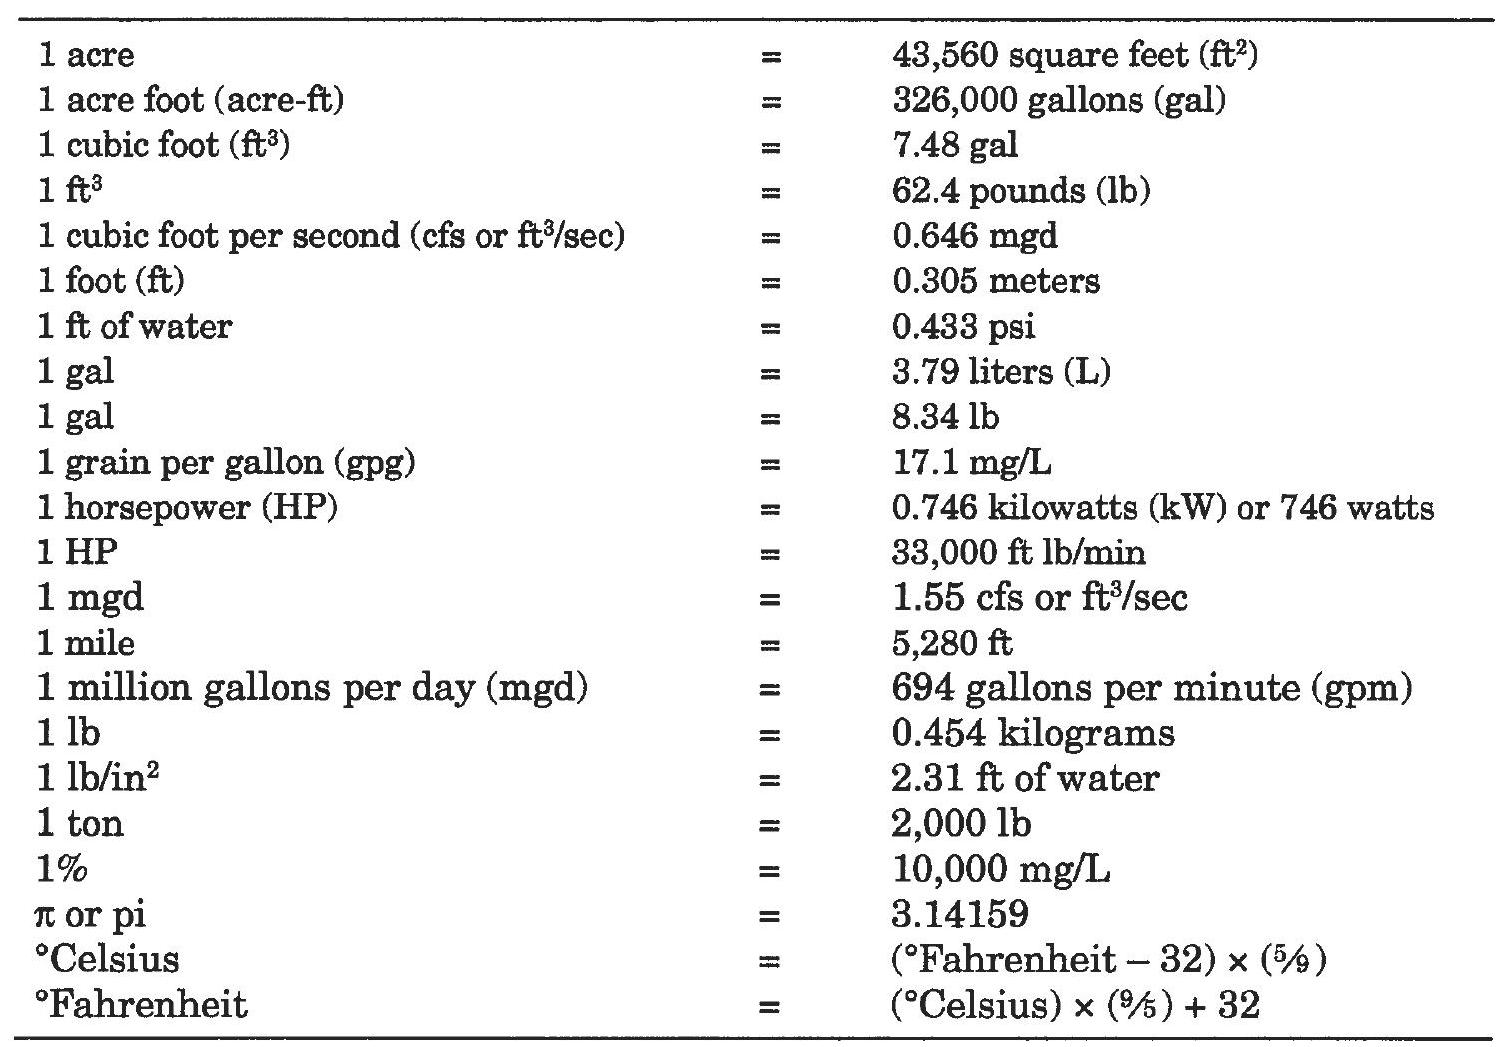
\includegraphics[max width=\textwidth]{2022_11_10_d6923b5a412978ed01fcg-59}

\section{Additional Abbreviations}
$\begin{array}{ll}\text { bhp } & \text { brake horsepower } \\ \text { DO } & \text { dissolved oxygen } \\ \text { EDTA } & \text { ethylenediaminetetraacetic acid } \\ \text { g } & \text { grams } \\ \text { gpcd } & \text { gallons per capita per day } \\ \text { gpd } & \text { gallons per day } \\ \text { in. } & \text { inch(es) } \\ \text { mg/L } & \text { milligrams per liter } \\ \text { mhp } & \text { motor horsepower } \\ \text { mil gal } & \text { million gallons } \\ \text { min } & \text { minute(s) } \\ \text { mL } & \text { milliliter } \\ \text { ppb } & \text { parts per billion } \\ \text { ppm } & \text { parts per million } \\ \text { psi } & \text { pounds per square inch } \\ \text { Q } & \text { low }\end{array}$

$\begin{array}{ll}\text { SS } & \text { settleable solids } \\ \text { TTHM } & \text { total trihalomethanes } \\ \text { TOC } & \text { total organic carbon } \\ \text { TSS } & \text { total suspended solids } \\ \text { VS } & \text { volatile solids } \\ \text { whp } & \text { water horsepower }\end{array}$

\section{Appendix B: Sample CT Tables for Giardia Inactivation}
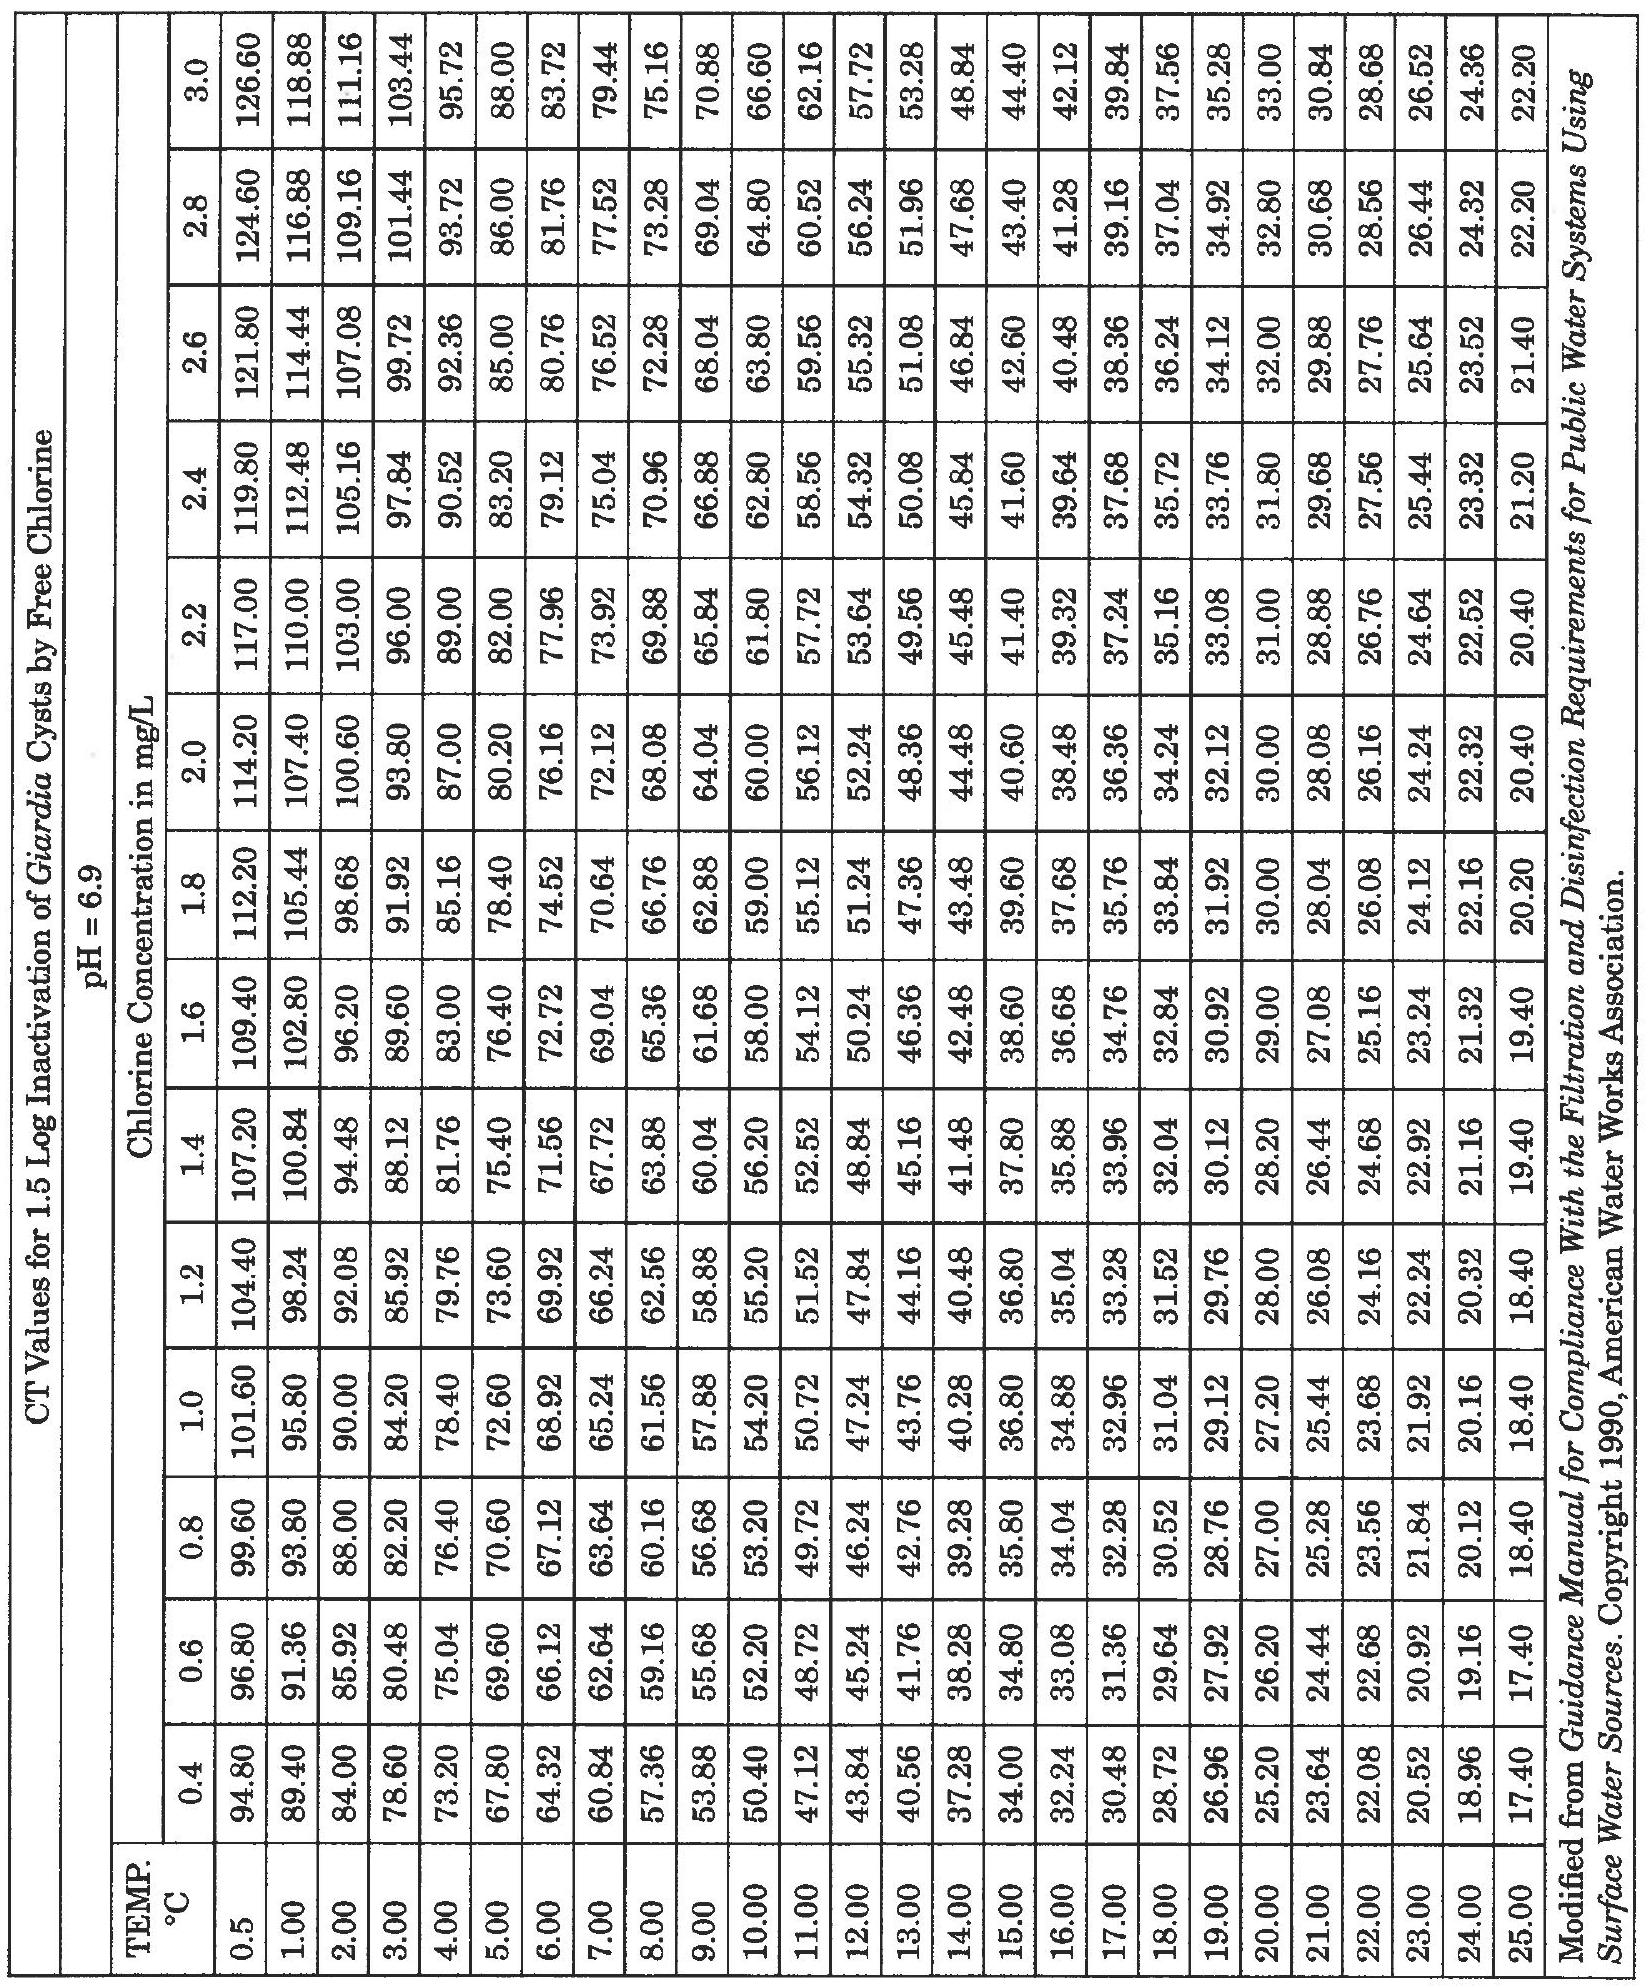
\includegraphics[max width=\textwidth]{2022_11_10_d6923b5a412978ed01fcg-61}

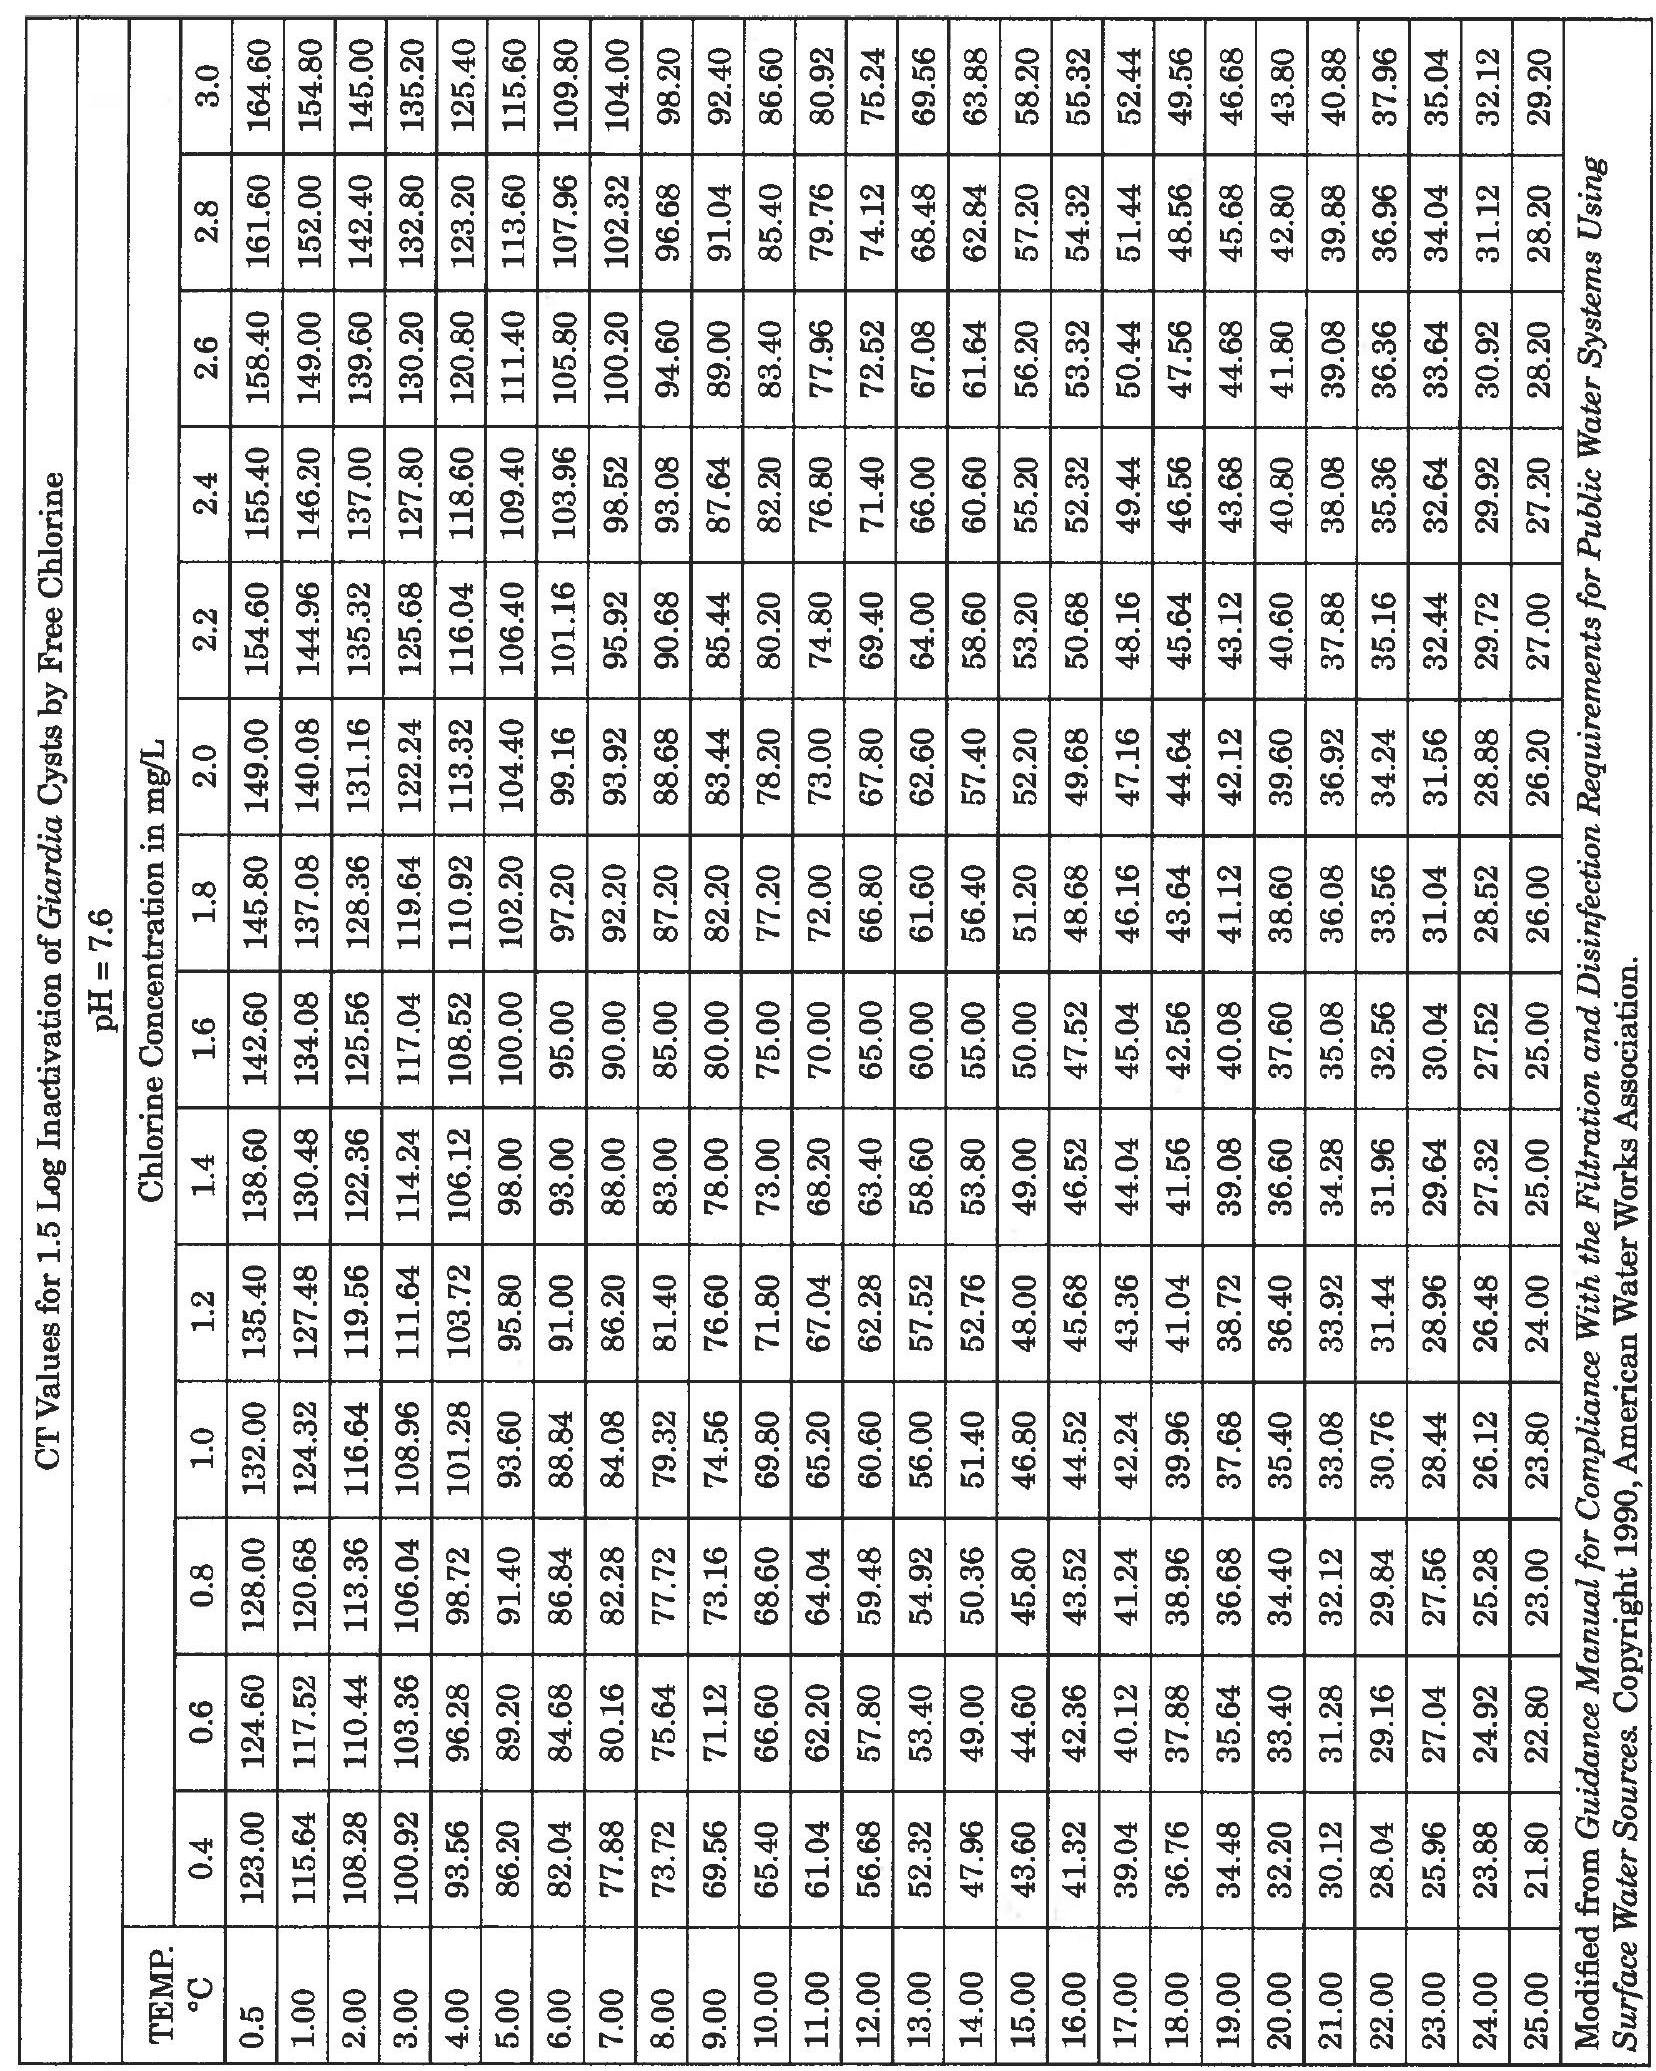
\includegraphics[max width=\textwidth]{2022_11_10_d6923b5a412978ed01fcg-62}

\section{Additional Resources}
The following items are all available from the AWWA Bookstore : \href{http://www.awwa.org/}{www.awwa.org/} bookstore; 1.800.926.7337; \href{mailto:custsve@awwa.org}{custsve@awwa.org}

Principles and Practices of Water Supply Operations (WSO): Water Sources, 4th edition. 2010. 192 pp. Hardback. 978-1-58321-782-5. Catalog No. 1955

WSO: Water Treatment, 4th edition. 2010. 512 pp. Hardback. 978-1-58321-777-1. Catalog No. 1956

Water Treatment Student Workbook, 4th edition. 2010. 120 pp. Softbound. 978-1-58321-794-8. Catalog No. 1966

WSO: Water Transmission and Distribution, 4th edition. 2010. 546 pp. Hardback. 978-1-58321-781-8. Catalog No. 1957

Water Transmission and Distribution Student Workbook, 4th edition. 2010. $114 \mathrm{pp}$. Softbound. 978-1-58321-800-6. Catalog No. 1967

WSO: Water Quality, 4th edition. 2010. 213 pp. Hardback. 978-1-58321-798-6. Catalog No. 1958

Water Quality Student Workbook, 4th edition. 2010. 63 pp. Softbound. 978-1-58321-794-8. Catalog No. 1968

WSO: Basic Science Concepts and Applications, 4th edition. 2010. 626 pp. Hardback. 978-1-58321-778-8. Catalog No. 1959

Basic Science Concepts and Applications Student Workbook, 4th edition. 2010. $200 \mathrm{pp}$. Softbound. 978-1-58321-799-3. Catalog No. 1954

Basic Chemistry for Water \& Wastewater Operators. 2005. Darshan Singh Sarai. 96 pp. Softbound. 978-1-58321-148-9. Catalog No. 20494

Basic Microbiology for Drinking Water Personnel, 2nd edition. 2006. Dennis Hill. 109 pp. Softbound. 978-1-58321-434-3. Catalog No. 20463

Math for Distribution System Operators. 2007. John Giorgi. $250 \mathrm{pp}$. Softbound. 978-1-58321-455-8. Catalog No. 20628

Math for Water Treatment Operators. 2007. John Giorgi. $250 \mathrm{pp}$. Softbound. 978-1-58321-454-1. Catalog No. 20618

Water Distribution Operator Training Handbook, 3rd edition. 2005. 286 pp. Softbound. 978-1-58321-372-8. Catalog No. 20428

Water Treatment Made Simple for Operators. 2006. Darshan Singh Sarai. 263 pp. Hardback. 978-0-47174-002-5. Catalog No. 20526

Water Treatment Operator Handbook. 2005. Nicholas G. Pizzi. 251 pp. Softbound. 978-1-58321-371-1. Catalog No. 20481

Water Distribution System Operation and Maintenance: A Field Study Training Program, 5th edition. 2005. 654 pp. Softbound. 978-1-59371-020-0. Catalog No. 20684

\section{Math \& Sclence}
\begin{itemize}
  \item Applled Mathematics .3 CEUs EL6

  \item Basic Mathematics 7 CEUs EL7

  \item Fundamentais of Chemistry for Water Professionals $.8$ CEUs EL12

  \item Things That Tripped Me Up on the Operator Certification Exam $.2$ CEUs EL88

\end{itemize}

\section{Quality}
\begin{itemize}
  \item Chlorine Gas: Balancing Public Health .2 CEUs EL21

  \item Disinfection By-Products: Recent Research Raises Concern .2 CEUs EL105

  \item Endocrine Disruptors; Pharmaceuticals, and Personal Care Products Actions and Communication $.2$ CEUs EL17

  \item Harmful Algal Blooms: Cyanobacteria .2 CEUs EL20

  \item Inorganic Treatment: Avoiding Inadvertent Noncompliance .2 CEUs EL102

  \item New Approaches for Assessing Microbial Threats .2 CEUs EL103

  \item Optimizing Water Distribution System Quality .2 CEUs EL101

  \item Perchlorate and Emerging Contaminants: Where Are We Now? 2 CEUs EL72

  \item Plant to Tap: the Importance of Disinfection .2 CEUs EL79

  \item Quagga/Zebra Mussel Control .2 CEUs EL70

\end{itemize}

\section{Resources \& Reuse}
\begin{itemize}
  \item GeoScience in Water Aquifers .2 CEUs EL78

  \item Water Shortages: Finding a Solution .2 CEUs EL73

\end{itemize}

\section{Treatment}
\begin{itemize}
  \item Best of Membrane Conference .2 CEUs EL81

  \item Chemicals: Best Practices for Quality Assurance $.2$ CEUs EL76

  \item Chlorine Gas an inherently Safer Technology .2 CEUs EL27

  \item Chlorine Gas: Balancing Public Health .2 CEUs EL21

  \item Coagulation, Flocculation, and Sedimentation Basic .3 CEUs EL8

  \item Disinfection Basics 3 CEUs EL9

  \item Filter Optimization Tips You Can Use .2CEUs EL107

  \item Flitration Basics 3 CEUs EL10

  \item High Tech Operator Course 1: Treatment \& Distribution - Process Monitoring and Control 1.2 CEUs EL84

  \item High Tech Operator Course 2: Application \& Tools $1.2$ CEUs EL85

  \item High Tech Operator Course 3: Data Management 1.2 CEUs EL86

  \item High Tech Operator Certificate Program 3.6 CEUs EL87

  \item Membranes: Emerging Issues \& Technologies .2 CEUs EL23

  \item Plant to Tap: The Importance of Disinfection 2 CEUs EL79

  \item Residuals Management and Disposal .2 CEUs EL77

\end{itemize}

For complete course descriptions and outlines, please visit \href{http://www.awwa.org/elearning}{www.awwa.org/elearning}. Titles subject to change. For a list of pre-approved courses for continuation education credits, please visit \href{http://www.awwa.org/elearning/ceus}{www.awwa.org/elearning/ceus}. For questions, please email \href{mailto:elearning@awwa.org}{elearning@awwa.org} or call 303.347.6204.


\end{document}